%%%%%%%%%%%%%%%%%%%%%%%%%%%%%%%%%%%%%%%%%%%%%%%%%%%%%%%%%%%%%%%
%% BRIEF VERSION OF OXFORD THESIS TEMPLATE FOR CHAPTER PREVIEWS

%%%%% CHOOSE PAGE LAYOUT
% format for PDF output (ie equal margins, no extra blank pages):
\documentclass[a4paper,nobind]{templates/ociamthesis}

% UL 5 January 2021 - add packages used by kableExtra
\usepackage{booktabs}
\usepackage{longtable}
\usepackage{array}
\usepackage{multirow}
\usepackage{wrapfig}
\usepackage{colortbl}
\usepackage{pdflscape}
\usepackage{tabu}
\usepackage{threeparttable}
\usepackage{threeparttablex}
\usepackage[normalem]{ulem}
\usepackage{makecell}
\usepackage[colorlinks=false,pdfpagelabels,hidelinks=]{hyperref}
\usepackage{float}


%UL set section header spacing
\usepackage{titlesec}
% 
\titlespacing\subsubsection{0pt}{24pt plus 4pt minus 2pt}{0pt plus 2pt minus 2pt}

% UL 30 Nov 2018 pandoc puts lists in 'tightlist' command when no space between bullet points in Rmd file
\providecommand{\tightlist}{%
  \setlength{\itemsep}{0pt}\setlength{\parskip}{0pt}}
 
% UL 1 Dec 2018, fix to include code in shaded environments
\usepackage{color}
\usepackage{fancyvrb}
\newcommand{\VerbBar}{|}
\newcommand{\VERB}{\Verb[commandchars=\\\{\}]}
\DefineVerbatimEnvironment{Highlighting}{Verbatim}{commandchars=\\\{\}}
% Add ',fontsize=\small' for more characters per line
\usepackage{framed}
\definecolor{shadecolor}{RGB}{248,248,248}
\newenvironment{Shaded}{\begin{snugshade}}{\end{snugshade}}
\newcommand{\AlertTok}[1]{\textcolor[rgb]{0.94,0.16,0.16}{#1}}
\newcommand{\AnnotationTok}[1]{\textcolor[rgb]{0.56,0.35,0.01}{\textbf{\textit{#1}}}}
\newcommand{\AttributeTok}[1]{\textcolor[rgb]{0.77,0.63,0.00}{#1}}
\newcommand{\BaseNTok}[1]{\textcolor[rgb]{0.00,0.00,0.81}{#1}}
\newcommand{\BuiltInTok}[1]{#1}
\newcommand{\CharTok}[1]{\textcolor[rgb]{0.31,0.60,0.02}{#1}}
\newcommand{\CommentTok}[1]{\textcolor[rgb]{0.56,0.35,0.01}{\textit{#1}}}
\newcommand{\CommentVarTok}[1]{\textcolor[rgb]{0.56,0.35,0.01}{\textbf{\textit{#1}}}}
\newcommand{\ConstantTok}[1]{\textcolor[rgb]{0.00,0.00,0.00}{#1}}
\newcommand{\ControlFlowTok}[1]{\textcolor[rgb]{0.13,0.29,0.53}{\textbf{#1}}}
\newcommand{\DataTypeTok}[1]{\textcolor[rgb]{0.13,0.29,0.53}{#1}}
\newcommand{\DecValTok}[1]{\textcolor[rgb]{0.00,0.00,0.81}{#1}}
\newcommand{\DocumentationTok}[1]{\textcolor[rgb]{0.56,0.35,0.01}{\textbf{\textit{#1}}}}
\newcommand{\ErrorTok}[1]{\textcolor[rgb]{0.64,0.00,0.00}{\textbf{#1}}}
\newcommand{\ExtensionTok}[1]{#1}
\newcommand{\FloatTok}[1]{\textcolor[rgb]{0.00,0.00,0.81}{#1}}
\newcommand{\FunctionTok}[1]{\textcolor[rgb]{0.00,0.00,0.00}{#1}}
\newcommand{\ImportTok}[1]{#1}
\newcommand{\InformationTok}[1]{\textcolor[rgb]{0.56,0.35,0.01}{\textbf{\textit{#1}}}}
\newcommand{\KeywordTok}[1]{\textcolor[rgb]{0.13,0.29,0.53}{\textbf{#1}}}
\newcommand{\NormalTok}[1]{#1}
\newcommand{\OperatorTok}[1]{\textcolor[rgb]{0.81,0.36,0.00}{\textbf{#1}}}
\newcommand{\OtherTok}[1]{\textcolor[rgb]{0.56,0.35,0.01}{#1}}
\newcommand{\PreprocessorTok}[1]{\textcolor[rgb]{0.56,0.35,0.01}{\textit{#1}}}
\newcommand{\RegionMarkerTok}[1]{#1}
\newcommand{\SpecialCharTok}[1]{\textcolor[rgb]{0.00,0.00,0.00}{#1}}
\newcommand{\SpecialStringTok}[1]{\textcolor[rgb]{0.31,0.60,0.02}{#1}}
\newcommand{\StringTok}[1]{\textcolor[rgb]{0.31,0.60,0.02}{#1}}
\newcommand{\VariableTok}[1]{\textcolor[rgb]{0.00,0.00,0.00}{#1}}
\newcommand{\VerbatimStringTok}[1]{\textcolor[rgb]{0.31,0.60,0.02}{#1}}
\newcommand{\WarningTok}[1]{\textcolor[rgb]{0.56,0.35,0.01}{\textbf{\textit{#1}}}}

%UL 2 Dec 2018 add a bit of white space before and after code blocks
\renewenvironment{Shaded}
{
  \vspace{10pt}%
  \begin{snugshade}%
}{%
  \end{snugshade}%
  \vspace{8pt}%
}
%UL 2 Dec 2018 reduce whitespace around verbatim environments
\usepackage{etoolbox}
\makeatletter
\preto{\@verbatim}{\topsep=0pt \partopsep=0pt }
\makeatother

%UL 28 Mar 2019, enable strikethrough
\usepackage[normalem]{ulem}

%UL use soul package for correction highlighting
\usepackage{soul}
\usepackage{xcolor}
\newcommand{\ctext}[3][RGB]{%
  \begingroup
  \definecolor{hlcolor}{#1}{#2}\sethlcolor{hlcolor}%
  \hl{#3}%
  \endgroup
}
\soulregister\ref7
\soulregister\cite7
\soulregister\autocite7
\soulregister\textcite7
\soulregister\pageref7

%UL 3 Nov 2019, avoid mysterious error from not having hyperref included
\usepackage{hyperref}

%%%%% SELECT YOUR DRAFT OPTIONS
% Three options going on here; use in any combination.  But remember to turn the first two off before
% generating a PDF to send to the printer!

% This adds a "DRAFT" footer to every normal page.  (The first page of each chapter is not a "normal" page.)

% This highlights (in blue) corrections marked with (for words) \mccorrect{blah} or (for whole
% paragraphs) \begin{mccorrection} . . . \end{mccorrection}.  This can be useful for sending a PDF of
% your corrected thesis to your examiners for review.  Turn it off, and the blue disappears.

%%%%% BIBLIOGRAPHY SETUP
% Note that your bibliography will require some tweaking depending on your department, preferred format, etc.
% The options included below are just very basic "sciencey" and "humanitiesey" options to get started.
% If you've not used LaTeX before, I recommend reading a little about biblatex/biber and getting started with it.
% If you're already a LaTeX pro and are used to natbib or something, modify as necessary.
% Either way, you'll have to choose and configure an appropriate bibliography format...

% The science-type option: numerical in-text citation with references in order of appearance.
% \usepackage[style=numeric-comp, sorting=none, backend=biber, doi=false, isbn=false]{biblatex}
% \newcommand*{\bibtitle}{References}

% The humanities-type option: author-year in-text citation with an alphabetical works cited.
% \usepackage[style=authoryear, sorting=nyt, backend=biber, maxcitenames=2, useprefix, doi=false, isbn=false]{biblatex}
% \newcommand*{\bibtitle}{Works Cited}

%UL 3 Dec 2018: set this from YAML in index.Rmd
\usepackage[style=numeric-comp, sorting=none, backend=biber, doi=false, isbn=false]{biblatex}
\newcommand*{\bibtitle}{References}

% This makes the bibliography left-aligned (not 'justified') and slightly smaller font.
\renewcommand*{\bibfont}{\raggedright\small}

% Change this to the name of your .bib file (usually exported from a citation manager like Zotero or EndNote).
\addbibresource{references.bib}

%%%%% YOUR OWN PERSONAL MACROS
% This is a good place to dump your own LaTeX macros as they come up.

% To make text superscripts shortcuts
	\renewcommand{\th}{\textsuperscript{th}} % ex: I won 4\th place
	\newcommand{\nd}{\textsuperscript{nd}}
	\renewcommand{\st}{\textsuperscript{st}}
	\newcommand{\rd}{\textsuperscript{rd}}

%%%%% THE ACTUAL DOCUMENT STARTS HERE
\begin{document}

%%%%% CHOOSE YOUR LINE SPACING HERE
% This is the official option.  Use it for your submission copy and library copy:
\setlength{\textbaselineskip}{22pt plus2pt}
% This is closer spacing (about 1.5-spaced) that you might prefer for your personal copies:
%\setlength{\textbaselineskip}{18pt plus2pt minus1pt}

% UL: You can set the general paragraph spacing here - I've set it to 2pt (was 0) so
% it's less claustrophobic
\setlength{\parskip}{2pt plus 1pt}

% Leave this line alone; it gets things started for the real document.
\setlength{\baselineskip}{\textbaselineskip}

% all your chapters and appendices will appear here
\begin{savequote}
Change has a considerable psychological impact on the human mind. To the
fearful it is threatening because it means that things may get worse. To
the hopeful it is encouraging because things may get better. To the
confident it is inspiring because the challenge exists to make things
better.
\end{savequote}



\hypertarget{transformation-of-microfinance-institutions-in-africa}{%
\chapter{Transformation of Microfinance Institutions in Africa}\label{transformation-of-microfinance-institutions-in-africa}}

\minitoc 

\newpage

\begin{quote}
\hypertarget{abstract}{%
\section{\texorpdfstring{\textbf{Abstract}}{Abstract}}\label{abstract}}

We examine the factors driving non-governmental organisation microfinance institutions to convert to the commercial, profit-oriented model. Using data from the World Bank and the International Monetary Fund (IMF), we ran logit, probit, and multinomial logit models with NGOs as the base outcome. At the firm level, age, size influence transformation. Legal tradition, institutional quality, and stock market development are significant factors at the country level. However, private credit to GDP and GDP growth rates are not significant drivers of conversion. Older firms are less likely to be NGOs, as are MFIs in civil law countries. Larger MFIs and MFIs located in countries with ``other'' legal traditions are more likely to be commercial. Institutional quality raises the chances of conversion, while stock market capitalisation relates negatively with transformation. Overall, the model does better than a null model, and the results remain robust to removing outliers.
\end{quote}

\newpage

\hypertarget{background}{%
\section{\texorpdfstring{\textbf{Background}}{Background}}\label{background}}

The modern micro-finance (MF) industry draws its popularity from the promise of providing appropriate and affordable financial services to the population under-served by mainstream financial intermediaries \autocite{morduch1999microfinance,morduch2000microfinance}. The motivation for reaching out to the unbanked draws from researchers and development practitioners view that financial inclusion leads to welfare improvements for the recipients. As examples, some scholars associate access to finance with more business start-ups, higher savings rate, improved health, less child mortality, and higher education attainment by the poor, although other scholars downplay these findings \autocite{klapper2015role,o2017systematic,shahriar2017lender}. Much of the initial efforts to provide financial services to the unbanked rested on Microfinance. Microfinance refers to either the practice of delivering appropriate and affordable financial facilities to the financially excluded or the providers of such services \autocite{ledgerwood2006transforming}.

Pioneer Microfinance Institutions (MFIs), like Grameen Bank, mostly operated as Non-Governmental Organisations (NGOs) following the welfare approach, where the profitability of the institution played second to availing financial services to the poor \autocite{chahine2010social,d2017ngos}. However, the paradigm shift is towards the financial systems approach where MFIs operate under market principles, leading to charges of ``financialisation'' of poverty \autocite{mader2015financialization}, with the relatively higher interest rates charged to the clients equated to a ``poverty penalty'' \autocite{chen2017microfinance}. Some scholars and practitioners argue that MFIs following the profit-oriented financial systems model, though more financially sustainable, are subject to ``mission drift''. Mission drift refers to situations where MFIs lessens their commitment to availing financial services to the financially excluded to pursue profits \autocite{jia2016commercialization,mia2017mission}.

However, given the social mission inherent in MF, MFIs following the financial systems approach risk their legitimacy in society and local and international donor community, a significant source of funding even for commercial MFIs \autocite{nason2018behavioral}. For these reasons, some researchers and development practitioners vouch for the welfare approach, where MFIs focus primarily on the mission to reach the financially excluded without emphasizing profits. Most MFIs following the welfare approach are non-governmental organizations (NGOs). Though not subject to mission drift, the NGO model is over-reliant on volatile local and international donor funds and government subsidies \autocite{garmaise2013cheap,d2017aid}. Additionally, NGOs may crowd out the efficient, market-based microfinance providers \autocite{kota2007}, which may hurt aggregate welfare in the long run.

The win-win school attempts to reconcile the financial systems and welfare approach to microfinance. Adherents of the win-win school postulate that it is possible to achieve both financial sustainability (that is, turn a profit) and, at the same time, reach the financially excluded \autocite{kodongo2013individual}. As a case in point, some researchers argue that MFIs could strive to generate profits by offering financial services to the relatively well-off at market rates. The MFIs could then use the returns to subsidise the provision of financial services to the poor under a form of price discrimination, leading to ``mission expansion'' as opposed to mission drift \autocite{mersland2010microfinance}.

Globally, the shift from the pure welfare approach of MF provision is gaining ground. Most of the transformed MFIs operate at some point on the continuum between the NGO, welfare model and the financial systems approach \autocite{armendariz2013subsidy,d2013unsubsidized,hishigsuren2006transformation}. It all started in 1992 in Bolivia when Prodem, an NGO, converted to a commercial bank, Bancosol \autocite{fernando2004micro,creedy2018types}. Since then, many MFIs worldwide have converted from NGOs to commercial firms seeking to make profits.

This article explores the factors that drive the transformation of MFIs from NGOs to for-profit firms in Africa. To this end, we use a panel dataset of 705 MFIs in Africa from the MIX pooled database, with additional data from the World Bank- the World Development Indicators (WDI), the Worldwide Governance Index (WGI), and the Global Financial Development Databases (GFDD). We focus on Africa given the relatively low levels of financial inclusion on the continent \autocite{demirguc2018global}and the shortcomings inherent in combining data from different regions that may yield results that are not actionable. As \textcite{d2017ngos} and \textcite{wang2015ownership} suggest, the nature and performance of MFIs are country-specific. Hence, research focusing on particular regions, countries or even firms could better inform policy making.

This article contributes to the literature in two main ways. First, the study sheds light on the drivers of the transformation of microfinance institutions in Africa. Much of the literature has not examined this phenomenon, focusing on the shift's consequences and how MFIs can balance financial and social missions \autocite{d2013unsubsidized,forkusam2014does,mia2017mission}. We believe that our analysis could form a reasonable starting point for analysing the transformation of MFIs in other regions or countries. Second, we detail the linkages between the drivers of micro-finance institutions' transformation, showing how they interact to change the likelihood of conversion. We highlight the pitfalls that bedevil analysis pools data from heterogeneous sources, which may mask crucial differences or similarities between the analysis units.

The rest of the article is structured as follows. Section 2 presents the theoretical underpinnings and empirical findings related to the study. Subsequently, in section 3, we offer a summary of findings before delving into the analysis method and results in sections 4 and 5, respectively. Section 6 concludes.

\hypertarget{related-literature}{%
\section{Related Literature}\label{related-literature}}

Much of the early literature on the institutional change of MFIs dealt with the theoretical, philosophical, and historical basis for the transformation of MFIs from NGOs to commercial firms and the potential impacts of such conversion {[}\textcite{campion1999institutional}; christen2001commercialization; \textcite{gutierrez201920}; \textcite{zaby2019science}{]}. Views of scholars regarding the transformation of MFIs drew from the institutional theory on the persistence and convergence in organisations, including change and de-institutionalisation within firms \autocite{scott2004institutional} and the dominance of neoliberalism after the end of the cold war \autocite{ostry2017}.

The institutional theory holds that the institutional environment is more influential in developing formal structures in organisations than market pressures \autocite{maggio1991}. Coercion is one form of pressure from the institutional environment that makes organisations adopt institutional structures and practices. Institutional theorists note that stakeholders could force firms to adopt specific organisational structures and practices without critical scrutiny to gain legitimacy in the institutional environment \autocite{scott2004institutional,martinez2017coercive}.

With this hindsight, \textcite{bateman2010doesn} traces the pressure to convert MFIs from NGOs to the commercial model to the rise of neo-liberalism and the insistence that firms be financially self-sufficient instead of relying on government subsidies and, in the case of MFIs, donor funds. The wave of economic liberalisation and privatisation commenced in the early 1990s due to neo-liberalism \autocite{silva1998neoliberalism}. Researchers point to pressure from financiers of MF such as USAID and the World Bank as a significant driver for the decision for MFIs to transform \autocite{ostry2017}.

However, given that MFIs have a social mission, the transition to a market-led positioning is bound to conflict with the social objectives and threaten the MF industry's legitimacy \autocite{ramus2017,nason2018behavioral}. Specifically, the quest to satisfy both financial objectives and the social mission is likely to conflict, which may cause ``mission drift'' \autocite{mersland2010microfinance,mia2017mission}, where MFIs give greater priority to profitability than outreach to the unbanked.

Nonetheless, the push from donors to transform MFIs seems to contradict the slow pace of the transformation. NGOs still form a substantial proportion of MFIs in Africa, accounting for 32\%, second only to Non-Bank Financial Institutions (NBFIs) at 40\% \autocite{market2018global}. A question arises regarding the factors behind the persistence of certain organisational forms of MFI provision in Africa and across the globe. \textcite{pashkova2016business} tackled this question. They found that the cooperative model is prevalent in economies with civil law systems, low inflation levels, and high economic growth rates.

In contrast, NGO type MFIs feature in countries with high inflation rates and low economic growth levels, meaning that NGOs help the poor cope during challenging economic times. The commercial banking model features most in economies with common law legal systems. However, the study by Pashkova, et al.~does not explicitly address the transformation question; factors that determine the transformation of MFIs from NGOs to a commercial model addressed this article.

The capacity of the capital markets and its antecedents may raise the propensity for the transformation of MFIs. MFIs located in countries with well-developed capital markets can efficiently issue debt and equity instruments and raise public deposits \autocite{allen2013resolving,allen2014african}. Available literature points to legal tradition, governance and education as drivers of financial development in a country \autocite{rajan1998financial,baltagi2009financial} and which, by extension, drives economic growth going by the financial development-economic growth nexus literature \autocite{claessens2003financial}. The size of an MFI in terms of assets base, structure, and tangibility could enhance its capital acquisition capacity in line with the trade-off theory of capital structure \autocite{barclay2005capital,gwatidzo2009corporate,ojah2016effects}.

\textcite{ledgerwood2006transforming} attribute the financing structure, hence the organisational form of an MFI, to the institutional life cycle. For instance, in the early stages, most MFIs operate as NGOs relying on donations and concessionary funds, given that commercial funders deem them too risky. Later, they supplement their funding through government subsidies and equity funding from NGOs and public investors. In the final consolidation phase, most MFIs rely on debt, using foreign donors as guarantees and deposits, and increasingly adopt the commercial model. Thus, the age of an MFI may have a bearing on both the capital structure and organisational structure, with firm-level, country and regional, disparities attributable to regulatory provisions relating to the ways MFIs can raise capital and historical legacies on saving and lending \autocite{bayai2016financing}. The agency conflict that follows the introduction of debt and equity brings to the fore the potential conflict between optimising financial returns and the quest to stick to the social mission of MFIs, the second central strand of research on MFI conversion \autocite{nurmakhanova2015trade,bayai2016financing,abdulai2017trade,awaworyi2018sustainability}.

Quality of institutions features prominently in explaining the investment climate in a country. The famed ``Lucas Paradox'' has primarily been explained away by the differences in, among others, the institutions, especially the capacity to enter into and enforce contracts and guarantees against state appropriation of private property - property rights \autocite{azemar2013has,goktan2015explanation}. MFI transformation connotes the entry of private, profit-oriented capital that seeks returns and favours countries with refined institutions. Moreover, researchers have variously cited the quality of institutions as drivers of the ease to which firms, MFIs included, can access private funds by fostering a well developed financial ecosystem \autocite{huang2010political,kaidi2019financial}. In this case, the financial system would include equity and debt markets where private investors could buy stakes in or lend funds to the MFIs that seek to go commercial. The next section highlights the results of the study.

\hypertarget{summary-of-results}{%
\section{Summary of Results}\label{summary-of-results}}

The output from analysis of the data shows that at the country level, it is legal tradition, stock markets development, and governance (institutional quality) that relate to the likelihood of the transformation of MFIs. At the firm level, the age and size of the MFI raise the probability of conversion. There is also a robust time trend towards commercialization of MFIs which points to increased acceptance of microfinance's financial systems approach. Regional disparities are also evident with North Africa represented by NGOs in the sample data, probably due to religious constraints. GDP growth rate and education levels are not significant determinants of the probability of transformation. However, like the stock market to GDP, private credit to GDP has a negative coefficient.

Precisely, the probability of an MFI transforming declines with the increase in age, with older MFIs more likely to follow the NGO model than younger MFIs. In contrast, bigger MFIs have a higher likelihood of transforming to the commercial model, while smaller MFIs retain the NGO status. Also, MFIs in common law countries have a higher chance of changing than those in civil law countries. However, it is MFIs located in countries with other legal traditions (that is, not civil or common - see Appendix 6) that have the highest probability of going commercial. Stock market development relates negatively with the likelihood of transformation of MFIs, likely because people in countries with well developed financial markets are more likely served by the mainstream financial system, relying less on microfinance. However, only stock market development is a significant driver, with private credit being a negative but insignificant driver of transformation. As expected, governance/ institutional quality positively relates to the chance of a conversion. Regionally, the sample data has only NGOs for North Africa, reflecting religious constraints to for-profit microfinance lending in majority Muslim countries. Importantly, there is a potent time trend towards commercialisation of MFIs which points to a triumph of the financial systems approach to microfinance over the welfare model. GDP growth rate shows mixed results but is insignificant. In the next section, we highlight the methodology applied in the study.

\begin{Shaded}
\begin{Highlighting}[]
\DocumentationTok{\#\# legal traditions }
\DocumentationTok{\#\#\# Common law countries in Africa}
\NormalTok{common }\OtherTok{\textless{}{-}} \FunctionTok{tibble}\NormalTok{(}\AttributeTok{country =} \FunctionTok{c}\NormalTok{(}\StringTok{"Botswana"}\NormalTok{, }\StringTok{"Gambia, The"}\NormalTok{, }\StringTok{"Ghana"}\NormalTok{, }\StringTok{"Kenya"}\NormalTok{, }\StringTok{"Lesotho"}\NormalTok{, }\StringTok{"Liberia"}\NormalTok{, }\StringTok{"Malawi"}\NormalTok{, }\StringTok{"Namibia"}\NormalTok{, }\StringTok{"Nigeria"}\NormalTok{, }\StringTok{"Sierra Leone"}\NormalTok{, }\StringTok{"South Africa"}\NormalTok{, }\StringTok{"South Sudan"}\NormalTok{, }\StringTok{"Sudan"}\NormalTok{, }\StringTok{"Eswatini"}\NormalTok{, }\StringTok{"Tanzania"}\NormalTok{, }\StringTok{"Uganda"}\NormalTok{, }\StringTok{"Zambia"}\NormalTok{, }\StringTok{"Zimbabwe"}\NormalTok{), }\AttributeTok{trad =} \FunctionTok{c}\NormalTok{(}\FunctionTok{rep}\NormalTok{(}\StringTok{"common"}\NormalTok{, }\DecValTok{18}\NormalTok{)))}

\DocumentationTok{\#\#\# Civil law countries in Africa}
\NormalTok{civil }\OtherTok{\textless{}{-}} \FunctionTok{tibble}\NormalTok{(}\AttributeTok{country =} \FunctionTok{c}\NormalTok{(}\StringTok{"Algeria"}\NormalTok{, }\StringTok{"Benin"}\NormalTok{, }\StringTok{"Burkina Faso"}\NormalTok{, }\StringTok{"Cameroon"}\NormalTok{, }\StringTok{"Central African Republic"}\NormalTok{, }\StringTok{"Chad"}\NormalTok{, }\StringTok{"Comoros"}\NormalTok{, }\StringTok{"Congo, Rep."}\NormalTok{, }\StringTok{"Cote d\textquotesingle{}Ivoire"}\NormalTok{, }\StringTok{"Gabon"}\NormalTok{, }\StringTok{"Guinea"}\NormalTok{, }\StringTok{"Madagascar"}\NormalTok{, }\StringTok{"Mali"}\NormalTok{, }\StringTok{"Mauritania"}\NormalTok{, }\StringTok{"Morocco"}\NormalTok{, }\StringTok{"Niger"}\NormalTok{, }\StringTok{"Senegal"}\NormalTok{, }\StringTok{"Togo"}\NormalTok{, }\StringTok{"Tunisia"}\NormalTok{), }\AttributeTok{trad =} \FunctionTok{c}\NormalTok{(}\FunctionTok{rep}\NormalTok{(}\StringTok{"civil"}\NormalTok{, }\DecValTok{19}\NormalTok{)))}

\DocumentationTok{\#\#\# Other legal traditions in Africa}
\NormalTok{others }\OtherTok{\textless{}{-}} \FunctionTok{tibble}\NormalTok{(}\AttributeTok{country =} \FunctionTok{c}\NormalTok{(}\StringTok{"Equatorial Guinea"}\NormalTok{, }\StringTok{"Angola"}\NormalTok{, }\StringTok{"Burundi"}\NormalTok{, }\StringTok{"Cape Verde"}\NormalTok{, }\StringTok{"Congo, Dem. Rep."}\NormalTok{, }\StringTok{"Egypt, Arab Republic of"}\NormalTok{, }\StringTok{"Ethiopia"}\NormalTok{, }\StringTok{"Eritrea"}\NormalTok{, }\StringTok{"Guinea{-}Bissau"}\NormalTok{, }\StringTok{"Mozambique"}\NormalTok{, }\StringTok{"Rwanda"}\NormalTok{), }\AttributeTok{trad =} \FunctionTok{c}\NormalTok{(}\FunctionTok{rep}\NormalTok{(}\StringTok{"others"}\NormalTok{, }\DecValTok{11}\NormalTok{)))}

\DocumentationTok{\#\#\#Putting them all together}
\NormalTok{legal }\OtherTok{\textless{}{-}} \FunctionTok{rbind}\NormalTok{(common, civil, others)}
\end{Highlighting}
\end{Shaded}

\begin{Shaded}
\begin{Highlighting}[]
\CommentTok{\# Bond market data {-} private and public bond market capitalization to GDP}
\NormalTok{bonds }\OtherTok{\textless{}{-}} \FunctionTok{read\_excel}\NormalTok{(}\StringTok{"bonds\_oluoch.xlsx"}\NormalTok{) }\SpecialCharTok{\%\textgreater{}\%} 
  
\NormalTok{  janitor}\SpecialCharTok{::}\FunctionTok{clean\_names}\NormalTok{()}
\end{Highlighting}
\end{Shaded}

\begin{Shaded}
\begin{Highlighting}[]
\CommentTok{\# Add the financial development index to the dataset}
\DocumentationTok{\#\# Countries not part of Africa}
\NormalTok{mideast }\OtherTok{\textless{}{-}} \FunctionTok{c}\NormalTok{(}\StringTok{"Bahrain"}\NormalTok{, }\StringTok{"Iran, Islamic Rep."}\NormalTok{, }\StringTok{"Iraq"}\NormalTok{, }\StringTok{"Israel"}\NormalTok{, }\StringTok{"Jordan"}\NormalTok{, }\StringTok{"Kuwait"}\NormalTok{, }\StringTok{"Lebanon"}\NormalTok{, }\StringTok{"Malta"}\NormalTok{, }\StringTok{"Oman"}\NormalTok{, }\StringTok{"Qatar"}\NormalTok{, }\StringTok{"Saudi Arabia"}\NormalTok{, }\StringTok{"Syrian Arab Republic"}\NormalTok{, }\StringTok{"United Arab Emirates"}\NormalTok{, }\StringTok{"West Bank and Gaza"}\NormalTok{, }\StringTok{"Yemen, Rep."}\NormalTok{)}

\DocumentationTok{\#\# Load the financial structure data}
\NormalTok{finstr }\OtherTok{\textless{}{-}} \FunctionTok{read\_excel}\NormalTok{(}\StringTok{"FinancialStructureDatabase20191018.xlsx"}\NormalTok{, }\AttributeTok{sheet =} \DecValTok{4}\NormalTok{) }\SpecialCharTok{\%\textgreater{}\%} 
  
  \DocumentationTok{\#\# Select desired variables}
  \FunctionTok{select}\NormalTok{(country, region, year, pcrdbgdp, stmktcap, stvaltraded, stturnover, listco\_pc) }\SpecialCharTok{\%\textgreater{}\%} 
  
  \DocumentationTok{\#\#\# Filter out regions not in Africa or middle east}
  \FunctionTok{filter}\NormalTok{(region }\SpecialCharTok{==} \StringTok{"Sub{-}Saharan Africa"} \SpecialCharTok{|}\NormalTok{ region }\SpecialCharTok{==} \StringTok{"Middle East \& North Africa"}\NormalTok{) }\SpecialCharTok{\%\textgreater{}\%} 
  \DocumentationTok{\#\#\# Filter out countries in middle east and select year 1999 onwards}
  \FunctionTok{filter}\NormalTok{(}\SpecialCharTok{!}\NormalTok{country }\SpecialCharTok{\%in\%}\NormalTok{ mideast, year }\SpecialCharTok{\textgreater{}=} \DecValTok{1999}\NormalTok{) }\SpecialCharTok{\%\textgreater{}\%} 
  
\DocumentationTok{\#\# Replace NAs}
          \FunctionTok{group\_by}\NormalTok{(country) }\SpecialCharTok{\%\textgreater{}\%} 
  
          \FunctionTok{mutate}\NormalTok{(}\AttributeTok{pcrdbgdp =} \FunctionTok{replace\_na}\NormalTok{(pcrdbgdp, }\FunctionTok{median}\NormalTok{(pcrdbgdp, }\AttributeTok{na.rm =} \ConstantTok{TRUE}\NormalTok{)),}
                 
                 \AttributeTok{pcrdbgdp =} \FunctionTok{replace\_na}\NormalTok{(pcrdbgdp, }\DecValTok{0}\NormalTok{),}
                 
                 \AttributeTok{stmktcap =} \FunctionTok{replace\_na}\NormalTok{(stmktcap, }\FunctionTok{median}\NormalTok{(stmktcap, }\AttributeTok{na.rm =} \ConstantTok{TRUE}\NormalTok{)),}
                 
                 \AttributeTok{stmktcap =} \FunctionTok{replace\_na}\NormalTok{(stmktcap, }\DecValTok{0}\NormalTok{)) }\SpecialCharTok{\%\textgreater{}\%} \FunctionTok{ungroup}\NormalTok{() }\SpecialCharTok{\%\textgreater{}\%} 
  
\DocumentationTok{\#\# Join with the bonds data}
  \FunctionTok{left\_join}\NormalTok{(bonds, }\AttributeTok{by =} \FunctionTok{c}\NormalTok{(}\StringTok{"country"}\NormalTok{, }\StringTok{"year"}\NormalTok{)) }\SpecialCharTok{\%\textgreater{}\%} 
  
\DocumentationTok{\#\# rename bonds columns }
  \FunctionTok{rename}\NormalTok{(}\AttributeTok{prbonds =}\NormalTok{ outstanding\_t\_bonds\_percent\_gdp, }
         
         \AttributeTok{pubonds =}\NormalTok{ outstanding\_c\_bonds\_percent\_gdp) }\SpecialCharTok{\%\textgreater{}\%} 
  
  \DocumentationTok{\#\# Replace NAs in public bond and private bond markets }
  \FunctionTok{mutate}\NormalTok{(}\AttributeTok{pubonds =} \FunctionTok{replace\_na}\NormalTok{(pubonds, }\DecValTok{0}\NormalTok{), }
         
         \AttributeTok{prbonds =} \FunctionTok{replace\_na}\NormalTok{(prbonds, }\DecValTok{0}\NormalTok{)) }\SpecialCharTok{\%\textgreater{}\%} 
  
         \DocumentationTok{\#\# Rename Ivory Coast}
         \FunctionTok{mutate}\NormalTok{(}\AttributeTok{country =} \FunctionTok{if\_else}\NormalTok{(country }\SpecialCharTok{==} \StringTok{"Côte d\textquotesingle{}Ivoire"}\NormalTok{, }\StringTok{"Cote d\textquotesingle{}Ivoire"}\NormalTok{, }
                                  
\NormalTok{                                  country))}

\DocumentationTok{\#\# View missing data points}
\CommentTok{\#mice::md.pattern(finstr)}

\CommentTok{\#finstr \%\textgreater{}\% select(pcrdbgdp, stmktcap) \%\textgreater{}\% cor(.) \%\textgreater{}\% }
  
  \CommentTok{\#corrplot(method = "number", type = "lower")}
\end{Highlighting}
\end{Shaded}

\begin{Shaded}
\begin{Highlighting}[]
\DocumentationTok{\#\# Read in the dataset }
\NormalTok{my\_data }\OtherTok{\textless{}{-}} \FunctionTok{read\_csv}\NormalTok{(}\StringTok{"amelia.csv"}\NormalTok{) }\SpecialCharTok{\%\textgreater{}\%} 

\DocumentationTok{\#\# Region}
\FunctionTok{mutate}\NormalTok{(}\AttributeTok{region =} \FunctionTok{if\_else}\NormalTok{(region }\SpecialCharTok{==} \StringTok{"Middle East and North Africa"}\NormalTok{, }
                        
                        \StringTok{"North\_Africa"}\NormalTok{, region)) }\SpecialCharTok{\%\textgreater{}\%} 

\CommentTok{\# Clean the names }
\NormalTok{janitor}\SpecialCharTok{::}\FunctionTok{clean\_names}\NormalTok{() }\SpecialCharTok{\%\textgreater{}\%} 
  
\CommentTok{\# Set up factor variables }
\DocumentationTok{\#\# legal status }
\FunctionTok{mutate}\NormalTok{(}\AttributeTok{currentlegalstatus =} \FunctionTok{factor}\NormalTok{(currentlegalstatus, }
                           \AttributeTok{levels =} \FunctionTok{c}\NormalTok{(}\StringTok{"NGO"}\NormalTok{, }\StringTok{"Bank"}\NormalTok{, }\StringTok{"NBFI"}\NormalTok{, }
                            \StringTok{"Credit Union/ Cooperative"}\NormalTok{, }
                            \StringTok{"Rural Bank"}\NormalTok{)), }
      \DocumentationTok{\#\# Age}
      \AttributeTok{age =} \FunctionTok{factor}\NormalTok{(age, }\AttributeTok{levels =} \FunctionTok{c}\NormalTok{(}\StringTok{"New"}\NormalTok{, }\StringTok{"Young"}\NormalTok{, }\StringTok{"Mature"}\NormalTok{)),}
       
      \DocumentationTok{\#\# Region }
      \AttributeTok{region =} \FunctionTok{factor}\NormalTok{(region, }\AttributeTok{levels =} \FunctionTok{c}\NormalTok{(}\StringTok{"North\_Africa"}\NormalTok{, }\StringTok{"Africa"}\NormalTok{))) }\SpecialCharTok{\%\textgreater{}\%} 
  
      \DocumentationTok{\#\# Add the financial structure data     }
      \FunctionTok{left\_join}\NormalTok{(finstr, }\AttributeTok{by =} \FunctionTok{c}\NormalTok{(}\StringTok{"country"}\NormalTok{, }\StringTok{"year"}\NormalTok{)) }\SpecialCharTok{\%\textgreater{}\%} 
  
      \DocumentationTok{\#\# Add a binary variable for the legal dummy{-} NGO vs Others}
      \FunctionTok{mutate}\NormalTok{(}\AttributeTok{currentlegaldummy =} \FunctionTok{case\_when}\NormalTok{(currentlegalstatus }\SpecialCharTok{==} \StringTok{"NGO"} \SpecialCharTok{\textasciitilde{}} \StringTok{"NGO"}\NormalTok{,}
                                           
                                           \ConstantTok{TRUE} \SpecialCharTok{\textasciitilde{}} \StringTok{"others"}\NormalTok{),}
      
        \AttributeTok{currentlegaldummy =} \FunctionTok{factor}\NormalTok{(currentlegaldummy, }\AttributeTok{levels =} \FunctionTok{c}\NormalTok{(}\StringTok{"NGO"}\NormalTok{, }\StringTok{"others"}\NormalTok{)),}
        
        \AttributeTok{legal\_tradition =} \FunctionTok{factor}\NormalTok{(legal\_tradition, }
                                 
                                 \AttributeTok{levels =} \FunctionTok{c}\NormalTok{(}\StringTok{"Common"}\NormalTok{, }\StringTok{"Civil"}\NormalTok{, }\StringTok{"Other"}\NormalTok{))) }\SpecialCharTok{\%\textgreater{}\%} 
  \DocumentationTok{\#\# Select required variables }
  \FunctionTok{select}\NormalTok{(mfiid, mfiname, year, country, currentlegaldummy, currentlegalstatus, }
         
\NormalTok{         age, legal\_tradition, region.x, asset\_structure, }
         
\NormalTok{         assets, kkm, education, pcrdbgdp, stmktcap, prbonds, gdp\_growth\_annual) }\SpecialCharTok{\%\textgreater{}\%} 
  
          \DocumentationTok{\#\# Rename region}
         \FunctionTok{rename}\NormalTok{(}\AttributeTok{region =}\NormalTok{ region.x) }\SpecialCharTok{\%\textgreater{}\%} 
  
  \FunctionTok{group\_by}\NormalTok{(country) }\SpecialCharTok{\%\textgreater{}\%} 
  
  \FunctionTok{mutate}\NormalTok{(}\AttributeTok{kkm =} \FunctionTok{replace\_na}\NormalTok{(kkm, }\FunctionTok{median}\NormalTok{(kkm, }\AttributeTok{na.rm =} \ConstantTok{TRUE}\NormalTok{)),}
         \AttributeTok{education =} \FunctionTok{replace\_na}\NormalTok{(education, }\FunctionTok{median}\NormalTok{(education, }\AttributeTok{na.rm =} \ConstantTok{TRUE}\NormalTok{)),}
         \AttributeTok{prbonds =} \FunctionTok{replace\_na}\NormalTok{(prbonds, }\FunctionTok{median}\NormalTok{(prbonds, }\AttributeTok{na.rm =} \ConstantTok{TRUE}\NormalTok{)),}
         \AttributeTok{pcrdbgdp =} \FunctionTok{replace\_na}\NormalTok{(pcrdbgdp, }\FunctionTok{median}\NormalTok{(pcrdbgdp, }\AttributeTok{na.rm =} \ConstantTok{TRUE}\NormalTok{)),}
         \AttributeTok{stmktcap =} \FunctionTok{replace\_na}\NormalTok{(stmktcap, }\FunctionTok{median}\NormalTok{(stmktcap, }\AttributeTok{na.rm =} \ConstantTok{TRUE}\NormalTok{))) }\SpecialCharTok{\%\textgreater{}\%} 
  
  \FunctionTok{ungroup}\NormalTok{() }\SpecialCharTok{\%\textgreater{}\%} 
  
  \FunctionTok{group\_by}\NormalTok{(mfiid) }\SpecialCharTok{\%\textgreater{}\%} 
  
  \FunctionTok{mutate}\NormalTok{(}\AttributeTok{asset\_structure =} \FunctionTok{replace\_na}\NormalTok{(asset\_structure, }\FunctionTok{median}\NormalTok{(asset\_structure, }\AttributeTok{na.rm =} \ConstantTok{TRUE}\NormalTok{)), }\AttributeTok{assets =} \FunctionTok{replace\_na}\NormalTok{(assets, }\FunctionTok{median}\NormalTok{(assets, }\AttributeTok{na.rm =} \ConstantTok{TRUE}\NormalTok{))) }\SpecialCharTok{\%\textgreater{}\%} 
  
  \FunctionTok{ungroup}\NormalTok{() }\SpecialCharTok{\%\textgreater{}\%} 
  
  \FunctionTok{group\_by}\NormalTok{(region) }\SpecialCharTok{\%\textgreater{}\%} 
  
  \FunctionTok{mutate}\NormalTok{(}\AttributeTok{education =} \FunctionTok{replace\_na}\NormalTok{(education, }\FunctionTok{median}\NormalTok{(education, }\AttributeTok{na.rm =} \ConstantTok{TRUE}\NormalTok{)),}
         
         \AttributeTok{kkm =} \FunctionTok{replace\_na}\NormalTok{(kkm, }\FunctionTok{median}\NormalTok{(kkm, }\AttributeTok{na.rm =} \ConstantTok{TRUE}\NormalTok{)),}
         
         \AttributeTok{gdp\_growth\_annual =} \FunctionTok{replace\_na}\NormalTok{(gdp\_growth\_annual, }
                                        
         \FunctionTok{median}\NormalTok{(gdp\_growth\_annual, }\AttributeTok{na.rm =} \ConstantTok{TRUE}\NormalTok{))) }\SpecialCharTok{\%\textgreater{}\%} 
  
  \FunctionTok{ungroup}\NormalTok{() }\SpecialCharTok{\%\textgreater{}\%} 
  
  \FunctionTok{group\_by}\NormalTok{(currentlegalstatus) }\SpecialCharTok{\%\textgreater{}\%} 
  
  \FunctionTok{mutate}\NormalTok{(}\AttributeTok{assets =} \FunctionTok{replace\_na}\NormalTok{(assets, }\FunctionTok{median}\NormalTok{(assets, }\AttributeTok{na.rm =} \ConstantTok{TRUE}\NormalTok{))) }\SpecialCharTok{\%\textgreater{}\%} 
  
  \FunctionTok{ungroup}\NormalTok{() }\SpecialCharTok{\%\textgreater{}\%} 
  
  \FunctionTok{mutate}\NormalTok{(}\AttributeTok{dummy =} \FunctionTok{if\_else}\NormalTok{(currentlegaldummy }\SpecialCharTok{==} \StringTok{"NGO"}\NormalTok{, }\DecValTok{0}\NormalTok{, }\DecValTok{1}\NormalTok{)) }\SpecialCharTok{\%\textgreater{}\%} 
  
  \FunctionTok{mutate}\NormalTok{(}\AttributeTok{assets =} \FunctionTok{log}\NormalTok{(assets }\SpecialCharTok{+} \DecValTok{1}\NormalTok{),}
         
         \AttributeTok{pcrdbgdp =} \FunctionTok{log}\NormalTok{(pcrdbgdp }\SpecialCharTok{+} \DecValTok{1}\NormalTok{),}
         
         \AttributeTok{stmktcap =} \FunctionTok{log}\NormalTok{(stmktcap }\SpecialCharTok{+} \DecValTok{1}\NormalTok{),}
         
         \AttributeTok{prbonds =} \FunctionTok{log}\NormalTok{(prbonds }\SpecialCharTok{+} \DecValTok{1}\NormalTok{)) }\SpecialCharTok{\%\textgreater{}\%} 
  
  \FunctionTok{select}\NormalTok{(}\SpecialCharTok{{-}}\NormalTok{asset\_structure) }\SpecialCharTok{\%\textgreater{}\%} 
  
  \FunctionTok{add\_count}\NormalTok{(mfiid, }\AttributeTok{name =} \StringTok{"count"}\NormalTok{) }\SpecialCharTok{\%\textgreater{}\%} 
  
  \FunctionTok{mutate}\NormalTok{(}\AttributeTok{currentlegalstatus =} \FunctionTok{fct\_recode}\NormalTok{(currentlegalstatus, }\AttributeTok{Coop =} \StringTok{"Credit Union/ Cooperative"}\NormalTok{))}
\end{Highlighting}
\end{Shaded}

\begin{verbatim}
## Warning: Missing column names filled in: 'X1' [1]
\end{verbatim}

\begin{verbatim}
## 
## -- Column specification --------------------------------------------------------
## cols(
##   .default = col_double(),
##   mfiname = col_character(),
##   region = col_character(),
##   country = col_character(),
##   currentlegalstatus = col_character(),
##   outreach = col_character(),
##   age = col_character(),
##   period_type = col_character(),
##   currency = col_character(),
##   as_of_date = col_character(),
##   profit.status = col_character(),
##   sustainability = col_character(),
##   legal_tradition = col_character()
## )
## i Use `spec()` for the full column specifications.
\end{verbatim}

\begin{Shaded}
\begin{Highlighting}[]
\DocumentationTok{\#\# Write a csv for the data}
\NormalTok{my\_data }\SpecialCharTok{\%\textgreater{}\%} \FunctionTok{write.csv}\NormalTok{(., }\StringTok{"data.csv"}\NormalTok{)}

\DocumentationTok{\#\# Visualize missing data}
\CommentTok{\#md.pattern(data)}
\DocumentationTok{\#\# Amelia::missmap(data)}

\DocumentationTok{\#\# MFIs with three (3) or more years of data}
\NormalTok{data3 }\OtherTok{\textless{}{-}}\NormalTok{ my\_data }\SpecialCharTok{\%\textgreater{}\%} 
  
  \FunctionTok{group\_by}\NormalTok{(mfiid) }\SpecialCharTok{\%\textgreater{}\%} 
  
  \FunctionTok{filter}\NormalTok{(}\FunctionTok{n}\NormalTok{() }\SpecialCharTok{\textgreater{}} \DecValTok{3}\NormalTok{)}
  
\NormalTok{data3 }\SpecialCharTok{\%\textgreater{}\%} \FunctionTok{write.csv}\NormalTok{(., }\StringTok{"data3.csv"}\NormalTok{)}

\DocumentationTok{\#\# MFIs with three (3) or more years of data}
\NormalTok{data5 }\OtherTok{\textless{}{-}}\NormalTok{ my\_data }\SpecialCharTok{\%\textgreater{}\%} 
  
  \FunctionTok{group\_by}\NormalTok{(mfiid) }\SpecialCharTok{\%\textgreater{}\%} 
  
  \FunctionTok{filter}\NormalTok{(}\FunctionTok{n}\NormalTok{() }\SpecialCharTok{\textgreater{}} \DecValTok{5}\NormalTok{)  }
  
\NormalTok{data5 }\SpecialCharTok{\%\textgreater{}\%} \FunctionTok{write.csv}\NormalTok{(., }\StringTok{"data5.csv"}\NormalTok{)}
\end{Highlighting}
\end{Shaded}

\begin{Shaded}
\begin{Highlighting}[]
\DocumentationTok{\#\# Analysis function}
\NormalTok{panel\_logit }\OtherTok{\textless{}{-}} \ControlFlowTok{function}\NormalTok{(data, depvar, indepvars,}
                        \AttributeTok{effect =} \FunctionTok{c}\NormalTok{(}\StringTok{"individual"}\NormalTok{, }\StringTok{"time"}\NormalTok{, }\StringTok{"twoways"}\NormalTok{),}
                        \AttributeTok{model =} \FunctionTok{c}\NormalTok{(}\StringTok{"random"}\NormalTok{, }\StringTok{"pooling"}\NormalTok{, }\StringTok{"within"}\NormalTok{, }\StringTok{"between"}\NormalTok{),}
                        \AttributeTok{print.level =} \DecValTok{4}\NormalTok{,}
                        \AttributeTok{method =} \FunctionTok{c}\NormalTok{(}\StringTok{"bgfs"}\NormalTok{, }\StringTok{"nr"}\NormalTok{),}
                        \AttributeTok{family =} \FunctionTok{binomial}\NormalTok{(}\StringTok{\textquotesingle{}logit\textquotesingle{}}\NormalTok{),}
                        \AttributeTok{na.action =}\NormalTok{ na.rm, }
                        \AttributeTok{index =} \FunctionTok{c}\NormalTok{(}\StringTok{"mfiid"}\NormalTok{, }\StringTok{"year"}\NormalTok{))\{}
 
\NormalTok{   effect }\OtherTok{\textless{}{-}} \FunctionTok{match.arg}\NormalTok{(effect)}
\NormalTok{   model }\OtherTok{\textless{}{-}} \FunctionTok{match.arg}\NormalTok{(model)}
\NormalTok{   method }\OtherTok{\textless{}{-}} \FunctionTok{match.arg}\NormalTok{(method)}
   
  \FunctionTok{pglm}\NormalTok{(depvar }\SpecialCharTok{\textasciitilde{}}\NormalTok{ indepvars, }
       \AttributeTok{data =}\NormalTok{ data, }
       \AttributeTok{na.action =}\NormalTok{ na.action, }
       \AttributeTok{effect =}\NormalTok{ effect,}
       \AttributeTok{model =}\NormalTok{ model, }
       \AttributeTok{family =}\NormalTok{ family, }
       \AttributeTok{index =}\NormalTok{ index)}
\NormalTok{\}}
\end{Highlighting}
\end{Shaded}

\hypertarget{method}{%
\section{Method}\label{method}}

The article uses two approaches; the logit and probit models and the multinomial logit model, given that our dependent variable is discrete and error terms may not be normally distributed \autocite{cramer2002origins}. For the logit and probit models, MFIs following the NGO model take a code of zero and one for NBFIs, credit unions/ cooperatives, and rural banks. For the multinomial logit model, NGOs still take a zero code, with commercial banks, NBFIs, credit unions, and Rural Banks taking one, two, three, and four, respectively. The next section lays out and describes the models, variables, and data sources.

\hypertarget{the-model-variables-description-and-data-sources}{%
\subsection{The Model, Variables Description and Data Sources}\label{the-model-variables-description-and-data-sources}}

We use the model below to run both logit and probit regressions on a panel dataset of 705 MFIs in Africa. Assuming the error term \(\epsilon\) follows a logistic distribution \autocite{czepiel2002maximum}, we have,

\begin{equation}
y_{it} = log(\frac{p_{it}}{(1-p_{it})} ) = \alpha + x_{it} + \varepsilon_{it}
\end{equation}

where,

\begin{equation}
p_{it}  =  \frac{1}{1 +  e^{- z_{it} } } 
\end{equation}

and

\begin{equation}
1 + p_{it}  =  \frac{1}{1 +  e^{z_{it} } }
\end{equation}

for \(z_{it} = f(x_{it})\)

In the model, \(y_{it}\) is the current legal status of the MFI, the dependent variable. The dependent variable is a dummy with NGOs, the base outcome (coded zero), and other legal traditions take a code of one. The symbol \(x_{it}\) represents a vector of independent variables- age, size, capital market development, legal tradition, GDP growth rate, and institutional quality. Additionally, we include year dummies to cater to the trends towards commercialisation.

The multinomial logit model extends the binary logit model to more than two unordered levels (discrete choices). The data at hand meets the requirements for running a multinomial logit model as the dependent variable (the legal status of each MFI) has one outcome for each case. Also, the independent variables do not faultlessly predict the dependent variable \autocite{petrucci2009primer}. Suppose we have a dependent variable \(y\) consisting of \(K\) choices for \(K>=2\). Further, let the independent variables be \(x_1, x_2,………. x_n\), then we can specify the multinomial logit model as follows.

\begin{equation}
log(\frac{prob(k/X)}{prob(K/X)}) =   \beta_{0}^{k}  x_{0}  + \beta_{1}^{k}  x_{1} +  \cdots + \beta_{p}^{k}  x_{p}
\end{equation}

for \(k = 1 \cdots K-1\)

\(y\) is the dependent variable, in this case, one of NGO, commercial bank, NBFI, credit union or rural bank.

\(x\) is a vector of independent variables.

If \(K>2\), then we have a multinomial logit with \(K-1\) set of equations. Where \(K=2\), the model is the binary logit model denoted in equation one (1) where we have one equation. Note that in this case, we have arbitrarily assigned the last category (K) as the reference. Any other group can serve as a reference and hence not be part of the equations set.

One of the significant drawbacks of the multinomial logit is the violation of the assumption of the independence of irrelevant alternatives (IIA). \textcite{cheng2007testing} ) illustrate this assumption using the blue bus- red bus example. If the choice between car transport and a red bus, and given that the probability of choosing a bus is \(0.8\), and \(0.2\) for a car, then the bus's odds over car transport is 4. Suppose we introduce a third alternative, the blue bus. If the probabilities of choosing a red bus, blue bus, and car transport are \(0.6\), \(0.25\), \(0.15\), respectively, the assumption holds since the odds of selecting a red bus over a car are still \(4\). If the odds are different from \(4\), then the model violates the IIA, and the multinomial model is not fit for the data. In our case, we plausibly see the assumption holding because the legal status of an individual MFI is independent of the legal status of other MFIs. Table 1 (next page) describes the variables in detail.

\begin{Shaded}
\begin{Highlighting}[]
\FunctionTok{tribble}\NormalTok{(}\SpecialCharTok{\textasciitilde{}}\NormalTok{ Variable\_Description, }\StringTok{"1. Current Legal Status (Dependent Variable): This is the dependent variable. For logit and probit models, we create a dummy with the MFIs following the NGO Model getting a code of zero, and one in the case of non{-}bank financial institutions (NBFIs), rural banks, and credit unions/ cooperatives. We assign codes of zero to four for the multinomial logit model for NGOs, Banks, NBFIs, Cooperatives and Rural Banks, respectively. The data are available from the Microfinance Information Exchange, MIX (See source on note 1)."}\NormalTok{, }\StringTok{""}\NormalTok{, }\StringTok{"2.  Age: The period in which the MFI has been in operation. MFIs fall into one of three groups: new (1{-}4 years), young (4{-}8 years), and mature (over 8 years). The data are available from MIX."}\NormalTok{, }\StringTok{""}\NormalTok{, }\StringTok{"3. Legal Tradition (Legal): The indicator is a dummy variable with common law countries coded 0, civil law countries 1, and 2 otherwise as per the classification by Oto{-}Peralías and Romero{-}Ávila (2014)."}\NormalTok{, }\StringTok{""}\NormalTok{, }\StringTok{"4. Size (Log of Total Assets): We proxy the size of MFI with the natural logarithm of total assets, again using MIX data."}\NormalTok{, }\StringTok{""}\NormalTok{, }\StringTok{"5. Governance/ Institutional Quality (KKM): We take the first principal component of the WGI developed by Daniel Kaufmann, Aart Kraay and Massimo Mastruzzi (KKM) available on the World Bank\textquotesingle{}s Worldwide Governance Indicators, WGI (See source on note 3)."}\NormalTok{, }\StringTok{""}\NormalTok{, }\StringTok{"6. Private Credit to GDP: We capture the total amount of credit advanced to the private sector by financial intermediaries as a proxy for capital markets development concerning the banking sector following Ito and Kawai (2018). The data source is the Global Financial Development Database (GFDD) of the World Bank (See note 4)."}\NormalTok{, }\StringTok{""}\NormalTok{, }\StringTok{"7. Stock market capitalisation to GDP: We capture the  extent of stock market development using the ratio of stock market capitalisation to GDP to proxy how firms can raise equity capital. Although Africa\textquotesingle{}s equity markets are thin, some relatively large stock markets like South Africa, Kenya, and Ghana exist. The data are from the GFDD."}\NormalTok{, }\StringTok{""}\NormalTok{, }\StringTok{"8. GDP annual growth rate (GDP): This is the year on year growth in output adjusted for inflation and sourced from the World Development Indicators (WDI) (See note 2)."}\NormalTok{, }\StringTok{""}\NormalTok{, }\StringTok{"9. Education (EDUC): The indicator is a ratio of the gross enrolment in secondary school to the gross primary school enrolment as defined in the literature (Allen et al., 2013, 2014). The data are from the WDI."}\NormalTok{, }\StringTok{""}\NormalTok{) }\SpecialCharTok{\%\textgreater{}\%} 
  
  \FunctionTok{kbl}\NormalTok{(., }\AttributeTok{caption =} \StringTok{"Description of Variables"}\NormalTok{, }\AttributeTok{booktabs =} \ConstantTok{TRUE}\NormalTok{) }\SpecialCharTok{\%\textgreater{}\%} 
  
  \FunctionTok{kable\_paper}\NormalTok{(}\AttributeTok{full\_width =} \ConstantTok{TRUE}\NormalTok{) }\SpecialCharTok{\%\textgreater{}\%} 
  
  \FunctionTok{footnote}\NormalTok{(}\AttributeTok{number =} \FunctionTok{c}\NormalTok{(}\StringTok{"MIX Database on www.themix.org and https://datacatalog.worldbank.org/dataset/mix{-}market"}\NormalTok{, }\StringTok{"WDI on https://databank.worldbank.org/source/world{-}development{-}indicators."}\NormalTok{, }\StringTok{"WGI/ KKM on https://databank.worldbank.org/source/worldwide{-}governance{-}indicators."}\NormalTok{, }\StringTok{"GFDD on https://www.worldbank.org/en/publication/gfdr/data/global{-}financial{-}development{-}database"}\NormalTok{), }\AttributeTok{number\_title =} \StringTok{"Notes"}\NormalTok{,}
    
           \AttributeTok{general =} \StringTok{"Authors\textquotesingle{} construction from the literature"}\NormalTok{,}
           \AttributeTok{general\_title =} \StringTok{"Source: "}\NormalTok{)}
\end{Highlighting}
\end{Shaded}

\begin{table}

\caption{\label{tab:unnamed-chunk-8}Description of Variables}
\centering
\begin{tabu} to \linewidth {>{\raggedright}X}
\toprule
Variable\_Description\\
\midrule
1. Current Legal Status (Dependent Variable): This is the dependent variable. For logit and probit models, we create a dummy with the MFIs following the NGO Model getting a code of zero, and one in the case of non-bank financial institutions (NBFIs), rural banks, and credit unions/ cooperatives. We assign codes of zero to four for the multinomial logit model for NGOs, Banks, NBFIs, Cooperatives and Rural Banks, respectively. The data are available from the Microfinance Information Exchange, MIX (See source on note 1).\\
\\
2.  Age: The period in which the MFI has been in operation. MFIs fall into one of three groups: new (1-4 years), young (4-8 years), and mature (over 8 years). The data are available from MIX.\\
\\
3. Legal Tradition (Legal): The indicator is a dummy variable with common law countries coded 0, civil law countries 1, and 2 otherwise as per the classification by Oto-Peralías and Romero-Ávila (2014).\\
\addlinespace
\\
4. Size (Log of Total Assets): We proxy the size of MFI with the natural logarithm of total assets, again using MIX data.\\
\\
5. Governance/ Institutional Quality (KKM): We take the first principal component of the WGI developed by Daniel Kaufmann, Aart Kraay and Massimo Mastruzzi (KKM) available on the World Bank's Worldwide Governance Indicators, WGI (See source on note 3).\\
\\
\addlinespace
6. Private Credit to GDP: We capture the total amount of credit advanced to the private sector by financial intermediaries as a proxy for capital markets development concerning the banking sector following Ito and Kawai (2018). The data source is the Global Financial Development Database (GFDD) of the World Bank (See note 4).\\
\\
7. Stock market capitalisation to GDP: We capture the  extent of stock market development using the ratio of stock market capitalisation to GDP to proxy how firms can raise equity capital. Although Africa's equity markets are thin, some relatively large stock markets like South Africa, Kenya, and Ghana exist. The data are from the GFDD.\\
\\
8. GDP annual growth rate (GDP): This is the year on year growth in output adjusted for inflation and sourced from the World Development Indicators (WDI) (See note 2).\\
\addlinespace
\\
9. Education (EDUC): The indicator is a ratio of the gross enrolment in secondary school to the gross primary school enrolment as defined in the literature (Allen et al., 2013, 2014). The data are from the WDI.\\
\\
\bottomrule
\multicolumn{1}{l}{\rule{0pt}{1em}\textit{Source: }}\\
\multicolumn{1}{l}{\rule{0pt}{1em}Authors' construction from the literature}\\
\multicolumn{1}{l}{\rule{0pt}{1em}\textit{Notes}}\\
\multicolumn{1}{l}{\rule{0pt}{1em}\textsuperscript{1} MIX Database on www.themix.org and https://datacatalog.worldbank.org/dataset/mix-market}\\
\multicolumn{1}{l}{\rule{0pt}{1em}\textsuperscript{2} WDI on https://databank.worldbank.org/source/world-development-indicators.}\\
\multicolumn{1}{l}{\rule{0pt}{1em}\textsuperscript{3} WGI/ KKM on https://databank.worldbank.org/source/worldwide-governance-indicators.}\\
\multicolumn{1}{l}{\rule{0pt}{1em}\textsuperscript{4} GFDD on https://www.worldbank.org/en/publication/gfdr/data/global-financial-development-database}\\
\end{tabu}
\end{table}

\begin{Shaded}
\begin{Highlighting}[]
  \CommentTok{\#knitr::kable(caption = "Description of variables")}
\end{Highlighting}
\end{Shaded}

\hypertarget{results}{%
\section{Results}\label{results}}

\hypertarget{exploratory-data-analysis}{%
\subsection{Exploratory Data Analysis}\label{exploratory-data-analysis}}

In this section, we visualise the data and then summarise the variables in the model.

\hypertarget{data-visualisation}{%
\subsubsection{Data visualisation}\label{data-visualisation}}

Figure 1 below shows the summary statistics and scatter plots for the independent numeric variables. The summaries show a high correlation between education on the one hand and private bond market capitalisation to GDP, stock market capitalisation to GDP, and private credit to GDP on the other at around 0.5. As literature shows, higher education levels coincide with greater participation of individuals in capital markets as financial inclusion levels drop \autocite{allen2013resolving,allen2014african}. The stock market capitalisation to GDP and private bond market capitalisation to GDP correlates vastly, at 0.73, which indicates the concomitant maturity of capital markets. Typically, debt markets mature first, followed by stock markets and their development levels are correlated \autocite{levine1999stock}. Other variables that show a high correlation include private credit to GDP on the one hand and private bond market capitalisation to GDP, and stock market capitalisation to GDP at 0.32 and 0.47. Institutional quality (KKM) also correlates with education, private credit to GDP and private bond market capitalisation \autocite{yartey2008determinants}.

With this hindsight, we drop education and private bond market capitalisation from the model. Note that much of the private credit to GDP ratio's variation already reflected in the stock market to GDP ratio. Also, education reflects in general capital market development as documented in the literature. We also note that North Africa has only NGOs in the model, perhaps due to faith \autocite{allen2013resolving,allen2014african,hassan2018religious}. Hence, exclude region in the model. There could be country-specific effects that we capture using the quality of governance (KKM) \autocite{kunvcivc2014institutional} and the annual GDP growth rate \autocite{butkiewicz2006institutional}.

Figure 2 shows that mature MFIs dominate the dataset across all legal statuses and particularly dominant among rural banks, NGOs, and cooperatives. Turning to the prevalence of MFIs by legal status, cooperatives dominate civil law countries. Simultaneously, NGOs, NBFIs, commercial banks and rural banks are dominant in common law countries, which researchers have documented \autocite{pashkova2016business}. For other legal traditions, NBFIs and cooperatives dominate. As noted, North Africa has only NGOs in the dataset, which could indicate the religious constraints towards interest charging financial intermediaries \autocite{hassan2018religious}. Finally, while commercial banks and NBFIs show a higher asset base, NGOs and credit unions are not large. Commercial banks would be more extensive due to statutory minimum capital requirement resulting from their desire to optimise economies of scale \autocite{aiyar2016does}.

Turning to Figure 3, country-level governance matter more for commercial MFIs- commercial banks and NBFIs, compared to NGOs and rural banks in line with the link in the literature between investment, governance, and property rights \autocite{claessens2003financial}. Commercial banks, rural banks, and NGOs dominate countries with higher stock market development levels, while NBFIs and cooperatives trail, noting that cooperatives may be relatively less inclined to obtain funding from stock markets \autocite{porter1987economic}. The result could indicate the importance of equity capital for commercial banks and NGOs, while NBFIs tend to rely more on private equity and debt. Indeed, the data shows NBFIs dominate in countries where private credit to GDP is highest, followed by cooperatives and NGOs, while commercial banks and rural banks come last.

Lastly, commercial banks, NBFIs and rural banks tend to dominate countries with higher GDP growth rates. Higher GDP growth implies higher profitability which in turn allows commercial MFIs to thrive. Low GDP growth means that the not-for\_profit NGOs and member-oriented cooperatives tend to succeed as a cushion to the vulnerable in society and fill the void left by the commercial MFIs.

\newpage

\blandscape

\begin{Shaded}
\begin{Highlighting}[]
\NormalTok{my\_data }\SpecialCharTok{\%\textgreater{}\%}
  
  \FunctionTok{select}\NormalTok{(assets, kkm, education, }
         
\NormalTok{         pcrdbgdp, stmktcap, prbonds, gdp\_growth\_annual) }\SpecialCharTok{\%\textgreater{}\%} 
  
\NormalTok{         GGally}\SpecialCharTok{::}\FunctionTok{ggpairs}\NormalTok{() }\SpecialCharTok{+} \FunctionTok{labs}\NormalTok{(}\AttributeTok{title =} \StringTok{""}\NormalTok{, }
                                  
                                  \AttributeTok{caption =} \StringTok{"Source: Authors\textquotesingle{} construction from the literature"}\NormalTok{)}
\end{Highlighting}
\end{Shaded}

\begin{figure}
\centering
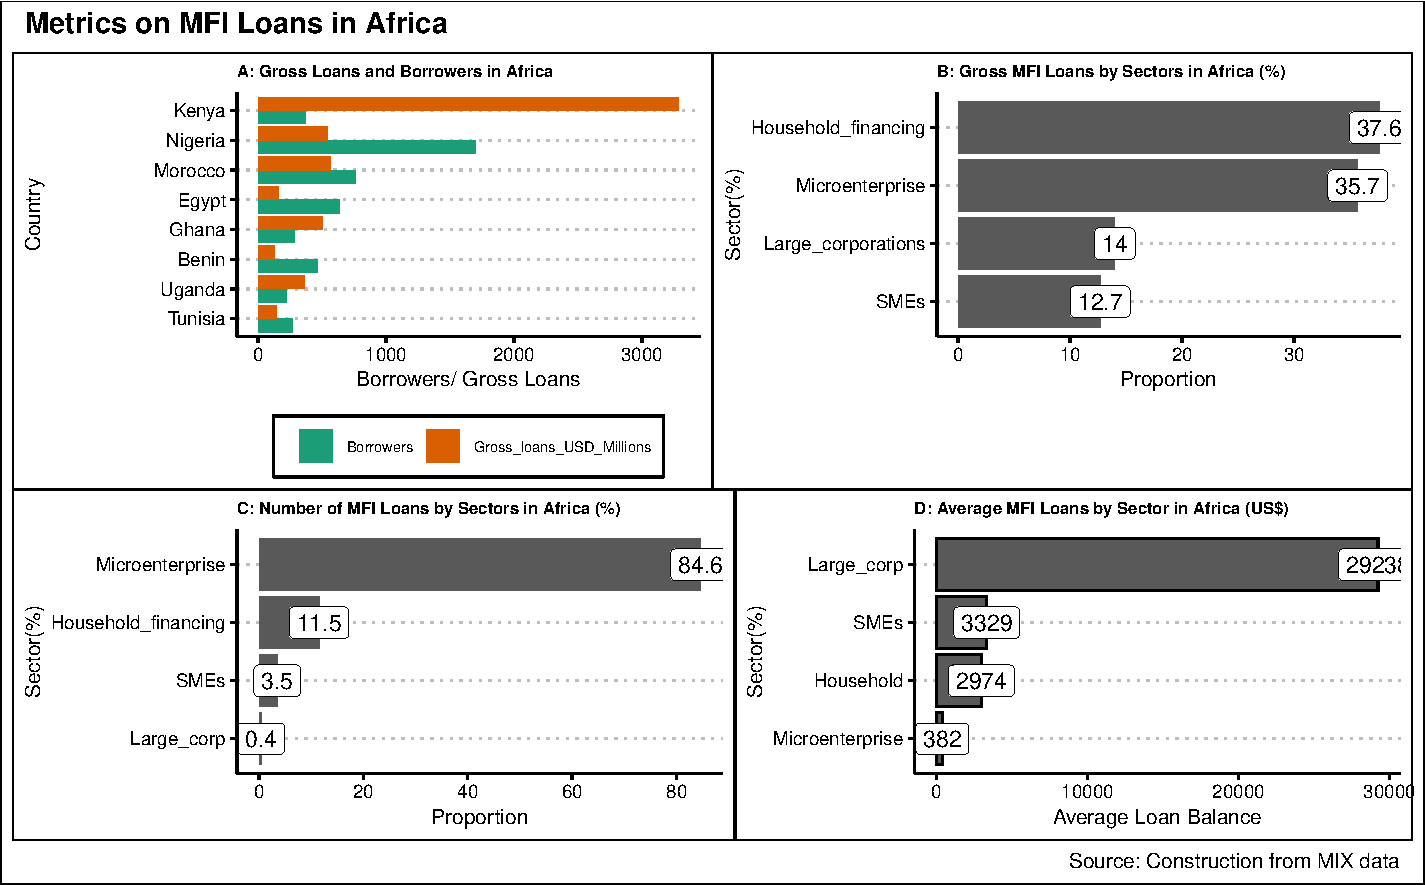
\includegraphics{05-extensions_files/figure-latex/unnamed-chunk-9-1.pdf}
\caption{\label{fig:unnamed-chunk-9}Correlations Between Independent Variables}
\end{figure}

\begin{Shaded}
\begin{Highlighting}[]
\CommentTok{\# Median function}
\NormalTok{median\_n }\OtherTok{\textless{}{-}} \ControlFlowTok{function}\NormalTok{(x)\{}\FunctionTok{median}\NormalTok{(x, }\AttributeTok{na.rm =} \ConstantTok{TRUE}\NormalTok{)\}}
\end{Highlighting}
\end{Shaded}

\begin{Shaded}
\begin{Highlighting}[]
\NormalTok{theme\_niwot }\OtherTok{\textless{}{-}} \ControlFlowTok{function}\NormalTok{()\{}
  \FunctionTok{theme\_bw}\NormalTok{() }\SpecialCharTok{+}
    \FunctionTok{theme}\NormalTok{(}\AttributeTok{axis.text =} \FunctionTok{element\_text}\NormalTok{(}\AttributeTok{size =} \DecValTok{7}\NormalTok{), }
          \AttributeTok{axis.title.x =} \FunctionTok{element\_blank}\NormalTok{(),}
          \AttributeTok{axis.title.y =} \FunctionTok{element\_text}\NormalTok{(}\AttributeTok{size =} \DecValTok{8}\NormalTok{),}
          \AttributeTok{axis.line.x =} \FunctionTok{element\_line}\NormalTok{(}\AttributeTok{color=}\StringTok{"black"}\NormalTok{), }
          \AttributeTok{axis.line.y =} \FunctionTok{element\_line}\NormalTok{(}\AttributeTok{color=}\StringTok{"black"}\NormalTok{),}
          \AttributeTok{panel.border =} \FunctionTok{element\_blank}\NormalTok{(),}
          \AttributeTok{panel.grid.major.x =} \FunctionTok{element\_blank}\NormalTok{(),                                          }
          \AttributeTok{panel.grid.minor.x =} \FunctionTok{element\_blank}\NormalTok{(),}
          \AttributeTok{panel.grid.minor.y =} \FunctionTok{element\_blank}\NormalTok{(),}
          \AttributeTok{panel.grid.major.y =} \FunctionTok{element\_blank}\NormalTok{(),  }
          \AttributeTok{plot.margin =} \FunctionTok{unit}\NormalTok{(}\FunctionTok{c}\NormalTok{(}\DecValTok{1}\NormalTok{, }\DecValTok{1}\NormalTok{, }\DecValTok{1}\NormalTok{, }\DecValTok{1}\NormalTok{), }\AttributeTok{units =}\NormalTok{ , }\StringTok{"cm"}\NormalTok{),}
          \AttributeTok{plot.title =} \FunctionTok{element\_text}\NormalTok{(}\AttributeTok{size =} \DecValTok{10}\NormalTok{, }\AttributeTok{vjust =} \DecValTok{1}\NormalTok{, }\AttributeTok{hjust =} \DecValTok{0}\NormalTok{),}
          \AttributeTok{legend.text =} \FunctionTok{element\_text}\NormalTok{(}\AttributeTok{size =} \DecValTok{8}\NormalTok{),          }
          \AttributeTok{legend.title =} \FunctionTok{element\_blank}\NormalTok{(),                              }
          \AttributeTok{legend.position =} \FunctionTok{c}\NormalTok{(}\FloatTok{0.95}\NormalTok{, }\FloatTok{0.15}\NormalTok{), }
          \AttributeTok{legend.key =} \FunctionTok{element\_blank}\NormalTok{(),}
          \AttributeTok{legend.background =} \FunctionTok{element\_rect}\NormalTok{(}\AttributeTok{color =} \StringTok{"black"}\NormalTok{, }
                                           \AttributeTok{fill =} \StringTok{"transparent"}\NormalTok{, }
                                           \AttributeTok{size =} \DecValTok{2}\NormalTok{, }\AttributeTok{linetype =} \StringTok{"blank"}\NormalTok{))}
\NormalTok{\}}
\end{Highlighting}
\end{Shaded}

\begin{Shaded}
\begin{Highlighting}[]
\DocumentationTok{\#\#\#\#\#\#\#\#\#\#\#\#\#\#\#\#\#\#\#\#\#\#\#\#\#\#\#\#\#\#\#\#\#\#\#\#\#\#\#\#\#\#\#}
\CommentTok{\#\textquotesingle{} ggplot Flat Violin}
\CommentTok{\#\textquotesingle{} @export}
\CommentTok{\#\textquotesingle{} @details Copy{-}pasted from https://gist.githubusercontent.com/benmarwick/2a1bb0133ff568cbe28d/raw/fb53bd97121f7f9ce947837ef1a4c65a73bffb3f/geom\_flat\_violin.R}
\CommentTok{\#\textquotesingle{} somewhat hackish solution to:}
\CommentTok{\#\textquotesingle{} https://twitter.com/EamonCaddigan/status/646759751242620928}
\CommentTok{\#\textquotesingle{} based mostly on copy/pasting from ggplot2 geom\_violin source:}
\CommentTok{\#\textquotesingle{} https://github.com/hadley/ggplot2/blob/master/R/geom{-}violin.r}
\CommentTok{\#\textquotesingle{} @examples:}
\CommentTok{\#\textquotesingle{} ggplot(diamonds, aes(cut, carat)) +}
\CommentTok{\#\textquotesingle{}   geom\_flat\_violin() +}
\CommentTok{\#\textquotesingle{}   coord\_flip()}
\CommentTok{\#\textquotesingle{} @import ggplot2}
\NormalTok{geom\_flat\_violin }\OtherTok{\textless{}{-}} \ControlFlowTok{function}\NormalTok{(}\AttributeTok{mapping =} \ConstantTok{NULL}\NormalTok{, }\AttributeTok{data =} \ConstantTok{NULL}\NormalTok{, }\AttributeTok{stat =} \StringTok{"ydensity"}\NormalTok{,}
                             \AttributeTok{position =} \StringTok{"dodge"}\NormalTok{, }\AttributeTok{trim =} \ConstantTok{TRUE}\NormalTok{, }\AttributeTok{scale =} \StringTok{"area"}\NormalTok{,}
                             \AttributeTok{show.legend =} \ConstantTok{NA}\NormalTok{, }\AttributeTok{inherit.aes =} \ConstantTok{TRUE}\NormalTok{, ...) \{}
  \FunctionTok{layer}\NormalTok{(}
    \AttributeTok{data =}\NormalTok{ data,}
    \AttributeTok{mapping =}\NormalTok{ mapping,}
    \AttributeTok{stat =}\NormalTok{ stat,}
    \AttributeTok{geom =}\NormalTok{ GeomFlatViolin,}
    \AttributeTok{position =}\NormalTok{ position,}
    \AttributeTok{show.legend =}\NormalTok{ show.legend,}
    \AttributeTok{inherit.aes =}\NormalTok{ inherit.aes,}
    \AttributeTok{params =} \FunctionTok{list}\NormalTok{(}
      \AttributeTok{trim =}\NormalTok{ trim,}
      \AttributeTok{scale =}\NormalTok{ scale,}
\NormalTok{      ...}
\NormalTok{    )}
\NormalTok{  )}
\NormalTok{\}}

\CommentTok{\#\textquotesingle{} @rdname ggplot2{-}ggproto}
\CommentTok{\#\textquotesingle{} @format NULL}
\CommentTok{\#\textquotesingle{} @usage NULL}
\CommentTok{\#\textquotesingle{} @export}
\NormalTok{GeomFlatViolin }\OtherTok{\textless{}{-}}
  \FunctionTok{ggproto}\NormalTok{(}\StringTok{"GeomFlatViolin"}\NormalTok{, Geom,}
          \AttributeTok{setup\_data =} \ControlFlowTok{function}\NormalTok{(data, params) \{}
\NormalTok{            data}\SpecialCharTok{$}\NormalTok{width }\OtherTok{\textless{}{-}}\NormalTok{ data}\SpecialCharTok{$}\NormalTok{width }\SpecialCharTok{\%||\%}
\NormalTok{              params}\SpecialCharTok{$}\NormalTok{width }\SpecialCharTok{\%||\%}\NormalTok{ (}\FunctionTok{resolution}\NormalTok{(data}\SpecialCharTok{$}\NormalTok{x, }\ConstantTok{FALSE}\NormalTok{) }\SpecialCharTok{*} \FloatTok{0.9}\NormalTok{)}

            \CommentTok{\# ymin, ymax, xmin, and xmax define the bounding rectangle for each group}
\NormalTok{            data }\SpecialCharTok{\%\textgreater{}\%}
              \FunctionTok{group\_by}\NormalTok{(group) }\SpecialCharTok{\%\textgreater{}\%}
              \FunctionTok{mutate}\NormalTok{(}\AttributeTok{ymin =} \FunctionTok{min}\NormalTok{(y),}
                     \AttributeTok{ymax =} \FunctionTok{max}\NormalTok{(y),}
                     \AttributeTok{xmin =}\NormalTok{ x,}
                     \AttributeTok{xmax =}\NormalTok{ x }\SpecialCharTok{+}\NormalTok{ width }\SpecialCharTok{/} \DecValTok{2}\NormalTok{)}

\NormalTok{          \},}

          \AttributeTok{draw\_group =} \ControlFlowTok{function}\NormalTok{(data, panel\_scales, coord) \{}
            \CommentTok{\# Find the points for the line to go all the way around}
\NormalTok{            data }\OtherTok{\textless{}{-}} \FunctionTok{transform}\NormalTok{(data, }\AttributeTok{xminv =}\NormalTok{ x,}
                              \AttributeTok{xmaxv =}\NormalTok{ x }\SpecialCharTok{+}\NormalTok{ violinwidth }\SpecialCharTok{*}\NormalTok{ (xmax }\SpecialCharTok{{-}}\NormalTok{ x))}

            \CommentTok{\# Make sure it\textquotesingle{}s sorted properly to draw the outline}
\NormalTok{            newdata }\OtherTok{\textless{}{-}} \FunctionTok{rbind}\NormalTok{(plyr}\SpecialCharTok{::}\FunctionTok{arrange}\NormalTok{(}\FunctionTok{transform}\NormalTok{(data, }\AttributeTok{x =}\NormalTok{ xminv), y),}
\NormalTok{                             plyr}\SpecialCharTok{::}\FunctionTok{arrange}\NormalTok{(}\FunctionTok{transform}\NormalTok{(data, }\AttributeTok{x =}\NormalTok{ xmaxv), }\SpecialCharTok{{-}}\NormalTok{y))}

            \CommentTok{\# Close the polygon: set first and last point the same}
            \CommentTok{\# Needed for coord\_polar and such}
\NormalTok{            newdata }\OtherTok{\textless{}{-}} \FunctionTok{rbind}\NormalTok{(newdata, newdata[}\DecValTok{1}\NormalTok{,])}

\NormalTok{            ggplot2}\SpecialCharTok{:::}\FunctionTok{ggname}\NormalTok{(}\StringTok{"geom\_flat\_violin"}\NormalTok{, GeomPolygon}\SpecialCharTok{$}\FunctionTok{draw\_panel}\NormalTok{(newdata, panel\_scales, coord))}
\NormalTok{          \},}

          \AttributeTok{draw\_key =}\NormalTok{ draw\_key\_polygon,}

          \AttributeTok{default\_aes =} \FunctionTok{aes}\NormalTok{(}\AttributeTok{weight =} \DecValTok{1}\NormalTok{, }\AttributeTok{colour =} \StringTok{"grey20"}\NormalTok{, }\AttributeTok{fill =} \StringTok{"white"}\NormalTok{, }\AttributeTok{size =} \FloatTok{0.5}\NormalTok{,}
                            \AttributeTok{alpha =} \ConstantTok{NA}\NormalTok{, }\AttributeTok{linetype =} \StringTok{"solid"}\NormalTok{),}

          \AttributeTok{required\_aes =} \FunctionTok{c}\NormalTok{(}\StringTok{"x"}\NormalTok{, }\StringTok{"y"}\NormalTok{)}
\NormalTok{  )}


\StringTok{"\%||\%"} \OtherTok{\textless{}{-}} \ControlFlowTok{function}\NormalTok{(a, b) \{}
  \ControlFlowTok{if}\NormalTok{ (}\SpecialCharTok{!}\FunctionTok{is.null}\NormalTok{(a)) a }\ControlFlowTok{else}\NormalTok{ b}
\NormalTok{\}}
\DocumentationTok{\#\#\#\#\#\#\#\#\#\#\#\#\#\#\#\#\#\#\#\#\#\#\#\#\#\#\#\#\#\#\#\#\#\#\#\#\#\#\#\#\#\#\#\#\#\#\#\#\#\#\#\#\#\#\#\#\#\#\#}
\end{Highlighting}
\end{Shaded}

\begin{Shaded}
\begin{Highlighting}[]
\CommentTok{\# plotting function}
\NormalTok{plotter }\OtherTok{\textless{}{-}} \ControlFlowTok{function}\NormalTok{(data, x , y, z, xlabel, ylabel, title)\{}
  
  \FunctionTok{library}\NormalTok{(tidyverse)}
  \FunctionTok{library}\NormalTok{(ggthemes)}
  \FunctionTok{library}\NormalTok{(gghalves)}
  \FunctionTok{library}\NormalTok{(ggalt)  }
  \FunctionTok{library}\NormalTok{(ggrepel)  }\CommentTok{\# for annotations}
  \FunctionTok{library}\NormalTok{(viridis)  }\CommentTok{\# for nice colors}
  \FunctionTok{library}\NormalTok{(broom)  }\CommentTok{\# for cleaning up models}
  \FunctionTok{library}\NormalTok{(treemapify)  }\CommentTok{\# for making area graphs}
  \FunctionTok{library}\NormalTok{(wesanderson)  }\CommentTok{\# for nice colors}
  
  \FunctionTok{ggplot}\NormalTok{(}\AttributeTok{data =}\NormalTok{ data, }\AttributeTok{mapping =} \FunctionTok{aes}\NormalTok{(}\AttributeTok{x =} \FunctionTok{reorder}\NormalTok{(\{\{x\}\}, \{\{y\}\}, median\_n), }
  \AttributeTok{y =}\NormalTok{ \{\{y\}\}, }\AttributeTok{fill =}\NormalTok{ \{\{z\}\})) }\SpecialCharTok{+} 
  \FunctionTok{geom\_boxplot}\NormalTok{(}\AttributeTok{width =} \FloatTok{0.2}\NormalTok{, }\AttributeTok{outlier.shape =} \ConstantTok{NA}\NormalTok{, }\AttributeTok{alpha =} \FloatTok{0.8}\NormalTok{, }\FunctionTok{aes}\NormalTok{(}\AttributeTok{fill =}\NormalTok{ \{\{z\}\})) }\SpecialCharTok{+}
  \FunctionTok{geom\_half\_violin}\NormalTok{(}\AttributeTok{position =} \FunctionTok{position\_nudge}\NormalTok{(}\AttributeTok{x =} \FloatTok{0.2}\NormalTok{, }\AttributeTok{y =} \DecValTok{0}\NormalTok{), }\AttributeTok{alpha =} \FloatTok{0.8}\NormalTok{) }\SpecialCharTok{+} 
    \FunctionTok{geom\_point}\NormalTok{(}\AttributeTok{position =} \FunctionTok{position\_jitter}\NormalTok{(}\AttributeTok{width =} \FloatTok{0.15}\NormalTok{), }\AttributeTok{size =} \DecValTok{1}\NormalTok{, }\AttributeTok{alpha =} \FloatTok{0.1}\NormalTok{) }\SpecialCharTok{+} 
    \FunctionTok{scale\_y\_log10}\NormalTok{() }\SpecialCharTok{+} \FunctionTok{labs}\NormalTok{(}\AttributeTok{y =}\NormalTok{ ylabel, }\AttributeTok{x =}\NormalTok{ xlabel, }
  \AttributeTok{title =}\NormalTok{ title) }\SpecialCharTok{+} 
  \FunctionTok{theme\_niwot}\NormalTok{() }\SpecialCharTok{+} 
  \FunctionTok{theme}\NormalTok{(}\AttributeTok{legend.position =} \StringTok{"none"}\NormalTok{) }\SpecialCharTok{+} 
  \FunctionTok{stat\_summary}\NormalTok{(}\AttributeTok{fun =}\NormalTok{ mean, }\AttributeTok{geom =} \StringTok{"point"}\NormalTok{, }
                \AttributeTok{size =} \DecValTok{1}\NormalTok{, }\AttributeTok{color =} \StringTok{"red"}\NormalTok{)\}}

\DocumentationTok{\#\#\#\#\#\#\#\#\#\#\#\#\#\#\#\#\#\#\#\#\#\#\#\#\#\#\#\#\#\#\#\#\#\#\#\#\#\#\#\#\#\#\#\#\#\#\#\#\#\#}
\NormalTok{second\_plotter }\OtherTok{\textless{}{-}} \ControlFlowTok{function}\NormalTok{(data, x , y, z, xlabel, ylabel, title)\{}

\FunctionTok{library}\NormalTok{(ggalt)  }
\FunctionTok{library}\NormalTok{(ggrepel)  }\CommentTok{\# for annotations}
\FunctionTok{library}\NormalTok{(viridis)  }\CommentTok{\# for nice colours}
\FunctionTok{library}\NormalTok{(broom)  }\CommentTok{\# for cleaning up models}
\CommentTok{\# devtools::install\_github("wilkox/treemapify")}
\FunctionTok{library}\NormalTok{(treemapify)  }\CommentTok{\# for making area graphs}
\FunctionTok{library}\NormalTok{(wesanderson)  }\CommentTok{\# for nice colours}

  \FunctionTok{ggplot}\NormalTok{(}\AttributeTok{data =}\NormalTok{ data, }
           \AttributeTok{mapping =} \FunctionTok{aes}\NormalTok{(}\AttributeTok{x =} \FunctionTok{reorder}\NormalTok{(\{\{x\}\}, \{\{y\}\}, median\_n), }\AttributeTok{y =}\NormalTok{ \{\{y\}\}, }\AttributeTok{fill =}\NormalTok{ \{\{z\}\})) }\SpecialCharTok{+}
    
    \CommentTok{\# The half violins}
    \FunctionTok{geom\_flat\_violin}\NormalTok{(}\AttributeTok{position =} \FunctionTok{position\_nudge}\NormalTok{(}\AttributeTok{x =} \FloatTok{0.2}\NormalTok{, }\AttributeTok{y =} \DecValTok{0}\NormalTok{), }\AttributeTok{alpha =} \FloatTok{0.8}\NormalTok{) }\SpecialCharTok{+}
    
    \CommentTok{\# The points}
    \FunctionTok{geom\_point}\NormalTok{(}\FunctionTok{aes}\NormalTok{(}\AttributeTok{y =}\NormalTok{ \{\{y\}\}, }\AttributeTok{color =}\NormalTok{ \{\{x\}\}), }
    
    \AttributeTok{position =} \FunctionTok{position\_jitter}\NormalTok{(}\AttributeTok{width =} \FloatTok{0.15}\NormalTok{), }\AttributeTok{size =} \DecValTok{1}\NormalTok{, }\AttributeTok{alpha =} \FloatTok{0.1}\NormalTok{) }\SpecialCharTok{+}
    
    \CommentTok{\# The boxplots}
    \FunctionTok{geom\_boxplot}\NormalTok{(}\AttributeTok{width =} \FloatTok{0.2}\NormalTok{, }\AttributeTok{outlier.shape =} \ConstantTok{NA}\NormalTok{, }\AttributeTok{alpha =} \FloatTok{0.8}\NormalTok{) }\SpecialCharTok{+}
    
    \CommentTok{\# \textbackslash{}n adds a new line which creates some space between the axis and axis title}
    \FunctionTok{labs}\NormalTok{(}\AttributeTok{x =}\NormalTok{ xlabel, }\AttributeTok{y =}\NormalTok{ ylabel, }\AttributeTok{title =}\NormalTok{ title) }\SpecialCharTok{+}
    
    \CommentTok{\# Removing legends}
    \FunctionTok{guides}\NormalTok{(}\AttributeTok{fill =} \ConstantTok{FALSE}\NormalTok{, }\AttributeTok{color =} \ConstantTok{FALSE}\NormalTok{) }\SpecialCharTok{+}
    
    \CommentTok{\# Setting the limits of the y axis}
    \CommentTok{\#scale\_y\_continuous(limits = c(0, 1.2)) +}
    
    \CommentTok{\# Picking nicer colours}
    \FunctionTok{scale\_fill\_manual}\NormalTok{(}\AttributeTok{values =} \FunctionTok{c}\NormalTok{(}\StringTok{"\#5A4A6F"}\NormalTok{, }\StringTok{"\#E47250"}\NormalTok{,  }\StringTok{"\#EBB261"}\NormalTok{, }\StringTok{"\#9D5A6C"}\NormalTok{, }\StringTok{"\#FFFF80FF"}\NormalTok{)) }\SpecialCharTok{+}
    
    \FunctionTok{scale\_colour\_manual}\NormalTok{(}\AttributeTok{values =} \FunctionTok{c}\NormalTok{(}\StringTok{"\#5A4A6F"}\NormalTok{, }\StringTok{"\#E47250"}\NormalTok{,  }\StringTok{"\#EBB261"}\NormalTok{, }\StringTok{"\#9D5A6C"}\NormalTok{, }\StringTok{"\#FFFF80FF"}\NormalTok{)) }\SpecialCharTok{+}
    
    \FunctionTok{theme\_niwot}\NormalTok{() }\SpecialCharTok{+} \FunctionTok{scale\_y\_log10}\NormalTok{()}
\NormalTok{\}}

\DocumentationTok{\#\#\#\#\#\#\#\#\#\#\#\#\#\#\#\#\#\#\#\#\#\#\#\#\#\#\#\#\#\#\#\#\#\#\#\#\#\#\#\#\#\#\#\#\#\#\#\#\#\#}
\CommentTok{\# plotting scatter diagrams }
\NormalTok{plotter\_scatter }\OtherTok{\textless{}{-}} \ControlFlowTok{function}\NormalTok{(data, x, y, z, }
\NormalTok{                            xlab, ylab, title) \{}
  
  \CommentTok{\# Load libraries}
  \FunctionTok{library}\NormalTok{(tidyverse)}
  \FunctionTok{library}\NormalTok{(gghalves)}
  \FunctionTok{library}\NormalTok{(ggeasy)}
  \FunctionTok{library}\NormalTok{(ggthemes)}
  
  \CommentTok{\# write the function}
\NormalTok{  data }\SpecialCharTok{\%\textgreater{}\%} \FunctionTok{ggplot}\NormalTok{(}\FunctionTok{aes}\NormalTok{(}\AttributeTok{x =}\NormalTok{ \{\{x\}\}, }\AttributeTok{y =}\NormalTok{ \{\{y\}\}, }\AttributeTok{col =}\NormalTok{ \{\{z\}\})) }\SpecialCharTok{+} 
    
    \FunctionTok{geom\_point}\NormalTok{(}\AttributeTok{shape =} \DecValTok{1}\NormalTok{, }\AttributeTok{size =} \DecValTok{2}\NormalTok{) }\SpecialCharTok{+} 
    
    \FunctionTok{labs}\NormalTok{(}\AttributeTok{x =}\NormalTok{ xlab, }\AttributeTok{y =}\NormalTok{ ylab, }\AttributeTok{title =}\NormalTok{ title)}
\NormalTok{\}}
\end{Highlighting}
\end{Shaded}

\begin{Shaded}
\begin{Highlighting}[]
\DocumentationTok{\#\# Current legal status vs age}
\NormalTok{(my\_data }\SpecialCharTok{\%\textgreater{}\%} 
  
  \FunctionTok{ggplot}\NormalTok{(}\AttributeTok{mapping =} \FunctionTok{aes}\NormalTok{(}\AttributeTok{x =} \FunctionTok{fct\_rev}\NormalTok{(}\FunctionTok{fct\_infreq}\NormalTok{(currentlegalstatus)), }\AttributeTok{fill =}\NormalTok{ age)) }\SpecialCharTok{+} 
  
  \FunctionTok{geom\_bar}\NormalTok{() }\SpecialCharTok{+} \FunctionTok{scale\_fill\_brewer}\NormalTok{(}\AttributeTok{palette =} \DecValTok{7}\NormalTok{) }\SpecialCharTok{+} 
  
  \FunctionTok{labs}\NormalTok{(}\AttributeTok{x =} \StringTok{""}\NormalTok{, }\AttributeTok{y =} \StringTok{"Count"}\NormalTok{, }
       
       \AttributeTok{title =} \StringTok{"Panel A: Current Legal Status by Age"}\NormalTok{) }\SpecialCharTok{+} 
   
   \FunctionTok{theme}\NormalTok{(}\AttributeTok{legend.title =} \FunctionTok{element\_blank}\NormalTok{(), }\AttributeTok{legend.position =} \StringTok{"top"}\NormalTok{) }\SpecialCharTok{+} 


\DocumentationTok{\#\# Current legal status vs legal tradition}
\NormalTok{my\_data }\SpecialCharTok{\%\textgreater{}\%} 
  
\FunctionTok{ggplot}\NormalTok{(}\AttributeTok{mapping =} \FunctionTok{aes}\NormalTok{(}\AttributeTok{x =} \FunctionTok{fct\_rev}\NormalTok{(}\FunctionTok{fct\_infreq}\NormalTok{(currentlegalstatus)), }
                     
                     \AttributeTok{fill =}\NormalTok{ legal\_tradition)) }\SpecialCharTok{+} 
  
  \FunctionTok{geom\_bar}\NormalTok{() }\SpecialCharTok{+} 
  
  \FunctionTok{scale\_fill\_brewer}\NormalTok{(}\AttributeTok{palette =} \DecValTok{2}\NormalTok{) }\SpecialCharTok{+} 
  
  \FunctionTok{labs}\NormalTok{(}\AttributeTok{x =} \StringTok{""}\NormalTok{, }\AttributeTok{y =} \StringTok{""}\NormalTok{, }
       
       \AttributeTok{title =} \StringTok{"Panel B: Current Legal Status by Legal Tradition"}\NormalTok{) }\SpecialCharTok{+} 
  
  \FunctionTok{theme}\NormalTok{(}\AttributeTok{legend.title =} \FunctionTok{element\_blank}\NormalTok{(), }\AttributeTok{legend.position =} \StringTok{"top"}\NormalTok{)) }\SpecialCharTok{/}

\DocumentationTok{\#\# Current legal status vs region}
\NormalTok{(my\_data }\SpecialCharTok{\%\textgreater{}\%} 
  
\FunctionTok{ggplot}\NormalTok{(}\AttributeTok{mapping =} \FunctionTok{aes}\NormalTok{(}\AttributeTok{x =} \FunctionTok{fct\_rev}\NormalTok{(}\FunctionTok{fct\_infreq}\NormalTok{(currentlegalstatus)), }
                     
                     \AttributeTok{fill =}\NormalTok{ region)) }\SpecialCharTok{+} 
  
  \FunctionTok{geom\_bar}\NormalTok{() }\SpecialCharTok{+} 
  
  \FunctionTok{scale\_fill\_brewer}\NormalTok{(}\AttributeTok{palette =} \DecValTok{9}\NormalTok{) }\SpecialCharTok{+} 
  
  \FunctionTok{labs}\NormalTok{(}\AttributeTok{x =} \StringTok{"Current Legal Status"}\NormalTok{, }\AttributeTok{y =} \StringTok{"Count"}\NormalTok{, }
       
       \AttributeTok{title =} \StringTok{"Panel C: Current Legal Status by Region"}\NormalTok{) }\SpecialCharTok{+} 
  
  \FunctionTok{theme}\NormalTok{(}\AttributeTok{legend.title =} \FunctionTok{element\_blank}\NormalTok{(), }\AttributeTok{legend.position =} \StringTok{"top"}\NormalTok{) }\SpecialCharTok{+} 


\DocumentationTok{\#\# Current legal status vs assets}
\FunctionTok{second\_plotter}\NormalTok{(my\_data, }\AttributeTok{x =} \FunctionTok{fct\_reorder}\NormalTok{(currentlegalstatus, assets, median), }
           
          \AttributeTok{y =}\NormalTok{ assets, }\AttributeTok{z =}\NormalTok{ currentlegalstatus, }\AttributeTok{xlabel =} \StringTok{"Current Legal Status"}\NormalTok{, }
          
          \AttributeTok{ylabel =} \StringTok{"Assets"}\NormalTok{, }\AttributeTok{title =} \StringTok{"Panel D: Assets of MFIs by Legal Status"}\NormalTok{))  }\SpecialCharTok{+} 
  
  \FunctionTok{plot\_annotation}\NormalTok{(}\AttributeTok{title =} \StringTok{""}\NormalTok{, }\AttributeTok{caption =} \StringTok{"Source: Authors\textquotesingle{} construction from MIX data"}\NormalTok{)}
\end{Highlighting}
\end{Shaded}

\begin{figure}
\centering
\includegraphics{05-extensions_files/figure-latex/unnamed-chunk-14-1.pdf}
\caption{\label{fig:unnamed-chunk-14}Distribution and Asset Base of MFIs in Africa by Legal Status}
\end{figure}

\begin{Shaded}
\begin{Highlighting}[]
\DocumentationTok{\#\#\#\#\#\#\#\#\#\#\#\#\#\#\#\#\#\#\#\#\#\#\#\#\#\#\#\#\#\#\#\#\#\#\#\#\#\#\#}
\DocumentationTok{\#\# Current legal status vs governance}
\NormalTok{(}\FunctionTok{second\_plotter}\NormalTok{(my\_data, }\AttributeTok{x =} \FunctionTok{fct\_reorder}\NormalTok{(currentlegalstatus, kkm), }\AttributeTok{y =}\NormalTok{ kkm, }
               
               \AttributeTok{z =}\NormalTok{ currentlegalstatus, }
               
               \AttributeTok{xlabel =} \StringTok{"Legal Status"}\NormalTok{, }\AttributeTok{ylabel =} \StringTok{"Country Governance Index (KKM)"}\NormalTok{, }
               
               \AttributeTok{title =} \StringTok{"Panel A: Country Level Governance and MFI legal status"}\NormalTok{) }\SpecialCharTok{+}



\DocumentationTok{\#\#\#\#\#\#\#\#\#\#\#\#\#\#\#\#\#\#\#\#\#\#\#\#\#\#\#\#\#\#\#\#\#\#\#\#\#\#}
\DocumentationTok{\#\# Current legal status vs stock market capitalization}
\FunctionTok{second\_plotter}\NormalTok{(my\_data, }\AttributeTok{x =} \FunctionTok{fct\_reorder}\NormalTok{(currentlegalstatus, stmktcap), }\AttributeTok{y =}\NormalTok{ stmktcap, }
               
               \AttributeTok{z =}\NormalTok{ currentlegalstatus, }
               
               \AttributeTok{xlabel =} \StringTok{"Legal Status"}\NormalTok{, }\AttributeTok{ylabel =} \StringTok{"Stock Market Development"}\NormalTok{, }
               
               \AttributeTok{title =} \StringTok{"Panel B: Stock Market Development and Legal Status of MFIs"}\NormalTok{)) }\SpecialCharTok{/}




\DocumentationTok{\#\#\#\#\#\#\#\#\#\#\#\#\#\#\#\#\#\#\#\#\#\#\#\#\#\#\#\#\#\#\#\#\#\#\#\#\#\#\#\#\#\#\#\#\#\#\#\#}
\DocumentationTok{\#\# Current legal status vs Private credit to GDP}
\NormalTok{(}\FunctionTok{second\_plotter}\NormalTok{(my\_data, }\AttributeTok{x =} \FunctionTok{fct\_reorder}\NormalTok{(currentlegalstatus, pcrdbgdp), }\AttributeTok{y =}\NormalTok{ pcrdbgdp, }
               
               \AttributeTok{z =}\NormalTok{ currentlegalstatus, }
               
               \AttributeTok{xlabel =} \StringTok{"Legal Status"}\NormalTok{, }\AttributeTok{ylabel =} \StringTok{"Private Credit to GDP"}\NormalTok{, }
               
               \AttributeTok{title =} \StringTok{"Panel C: Private Credit to GDP and Legal Status of MFIs"}\NormalTok{) }\SpecialCharTok{+}


\DocumentationTok{\#\# Current legal status vs GDP growth }
\FunctionTok{second\_plotter}\NormalTok{(my\_data, }\AttributeTok{x =} \FunctionTok{fct\_reorder}\NormalTok{(currentlegalstatus, gdp\_growth\_annual), }
               
               \AttributeTok{y =}\NormalTok{ gdp\_growth\_annual, }
               
               \AttributeTok{z =}\NormalTok{ currentlegalstatus, }
               
               \AttributeTok{xlabel =} \StringTok{"Legal Status"}\NormalTok{, }\AttributeTok{ylabel =} \StringTok{"GDP Growth Rates (\% Annual)"}\NormalTok{, }
               
               \AttributeTok{title =} \StringTok{"Panel D: GDP Growth Rates and Legal Status of MFIs"}\NormalTok{)) }\SpecialCharTok{+}


\FunctionTok{plot\_annotation}\NormalTok{(}\AttributeTok{title =} \StringTok{""}\NormalTok{, }\AttributeTok{caption =} \StringTok{"Source: Authors\textquotesingle{} construction from MIX data }\SpecialCharTok{\textbackslash{}n}
\StringTok{                Arranged in Ascending order of the median score"}\NormalTok{)}
\end{Highlighting}
\end{Shaded}

\begin{verbatim}
## Warning in self$trans$transform(x): NaNs produced
\end{verbatim}

\begin{verbatim}
## Warning: Transformation introduced infinite values in continuous y-axis
\end{verbatim}

\begin{verbatim}
## Warning in self$trans$transform(x): NaNs produced
\end{verbatim}

\begin{verbatim}
## Warning: Transformation introduced infinite values in continuous y-axis
\end{verbatim}

\begin{verbatim}
## Warning in self$trans$transform(x): NaNs produced
\end{verbatim}

\begin{verbatim}
## Warning: Transformation introduced infinite values in continuous y-axis
\end{verbatim}

\begin{verbatim}
## Warning: Removed 2715 rows containing non-finite values (stat_ydensity).
\end{verbatim}

\begin{verbatim}
## Warning: Removed 2715 rows containing non-finite values (stat_boxplot).
\end{verbatim}

\begin{verbatim}
## Warning: Removed 2715 rows containing missing values (geom_point).
\end{verbatim}

\begin{verbatim}
## Warning: Transformation introduced infinite values in continuous y-axis

## Warning: Transformation introduced infinite values in continuous y-axis

## Warning: Transformation introduced infinite values in continuous y-axis
\end{verbatim}

\begin{verbatim}
## Warning: Removed 2694 rows containing non-finite values (stat_ydensity).
\end{verbatim}

\begin{verbatim}
## Warning: Removed 2694 rows containing non-finite values (stat_boxplot).
\end{verbatim}

\begin{verbatim}
## Warning in self$trans$transform(x): NaNs produced
\end{verbatim}

\begin{verbatim}
## Warning: Transformation introduced infinite values in continuous y-axis
\end{verbatim}

\begin{verbatim}
## Warning in self$trans$transform(x): NaNs produced
\end{verbatim}

\begin{verbatim}
## Warning: Transformation introduced infinite values in continuous y-axis
\end{verbatim}

\begin{verbatim}
## Warning in self$trans$transform(x): NaNs produced
\end{verbatim}

\begin{verbatim}
## Warning: Transformation introduced infinite values in continuous y-axis
\end{verbatim}

\begin{verbatim}
## Warning: Removed 177 rows containing non-finite values (stat_ydensity).
\end{verbatim}

\begin{verbatim}
## Warning: Removed 177 rows containing non-finite values (stat_boxplot).
\end{verbatim}

\begin{verbatim}
## Warning: Removed 175 rows containing missing values (geom_point).
\end{verbatim}

\begin{figure}
\centering
\includegraphics{05-extensions_files/figure-latex/unnamed-chunk-15-1.pdf}
\caption{\label{fig:unnamed-chunk-15}Governance, Capital Market Development and Legal Status of MFIs in Africa}
\end{figure}

\elandscape

\newpage

\hypertarget{summary-statistics}{%
\subsubsection{Summary Statistics}\label{summary-statistics}}

Categorical variables summarised in Table 2 have no missing values. There are 1,280 NGOs against 3502 MFIs that are either commercial banks (619), NBFIs (1318), cooperatives (1427), and rural banks (138). As noted, even with the transformation of MFIs, NGOs still form a substantial number of MFIs, with the country to country variations \autocite{d2017ngos}. While 2558 MFIs are mature, 1200 are new, and 1024 are young. The result may indicate a slowdown in the establishment of new MFIs as donations become more unreliable. 1877 MFIs are from common law countries, with Civil law countries accounting for 1849, while 1056 come from other legal traditions. It is notable, as shown in Appendix 6, that most countries in Africa are either common law (18) or civil law(19), with very few nations in the `other' legal traditions category (11) \autocite{oto2014distribution}. It is also worth noting that North Africa accounts for only 166 observations in the data against 4616 observations in the sample dataset. Table 3 shows the summary statistics for the numeric variables where assets, governance (KKM), and GDP growth rates account for the highest variation.

Table 4 and Table 7 shows that NGOs, NBFIs, and commercial banks dominate common law countries. In civil law countries, it is cooperatives, NGOs, and NFIs that are most prevalent. In other legal traditions, it is NBFIs and credit unions that dominate. The result could indicate that the relatively well-developed capital markets in common law countries allow private, for-profit MFIs to thrive while not displacing NGOs. It means that NGOs in common law countries mostly serve niche markets where commercial MFIs find it uneconomical to reach. Weak capital markets in civil law countries mean that cooperatives are central, with NGOs playing a significant role. Commercial MFIs like commercial banks and cooperatives presence is low due to capital constraints. Turning to age in Table 5, most of the mature MFIs in the sample data are cooperatives, NGOs, and commercial banks in that order, while most of the new MFIs are NBFIs, cooperatives and commercial banks, respectively. The results could indicate the increasing acceptance of the commercial model with newer MFIs going commercial. Table 6 shows the correlation between age and size, with larger MFIs more likely to be older.

\begin{Shaded}
\begin{Highlighting}[]
\DocumentationTok{\#\# Summary statistics for factor variables }
\NormalTok{my\_data }\SpecialCharTok{\%\textgreater{}\%} 
  
  \FunctionTok{select}\NormalTok{(currentlegaldummy, currentlegalstatus, }
         
\NormalTok{         age, legal\_tradition, region) }\SpecialCharTok{\%\textgreater{}\%} 
  
  \FunctionTok{skim\_without\_charts}\NormalTok{() }\SpecialCharTok{\%\textgreater{}\%} 
  
  \FunctionTok{select}\NormalTok{(}\SpecialCharTok{{-}}\NormalTok{complete\_rate, }\SpecialCharTok{{-}}\NormalTok{skim\_type, }\SpecialCharTok{{-}}\NormalTok{factor.ordered, }
         
         \SpecialCharTok{{-}}\NormalTok{n\_missing, }\SpecialCharTok{{-}}\NormalTok{factor.n\_unique) }\SpecialCharTok{\%\textgreater{}\%} 
  
  \FunctionTok{rename}\NormalTok{(}\AttributeTok{Variable =}\NormalTok{ skim\_variable, }
         
         \AttributeTok{Counts =}\NormalTok{ factor.top\_counts) }\SpecialCharTok{\%\textgreater{}\%} 
  
\NormalTok{kableExtra}\SpecialCharTok{::}\FunctionTok{kbl}\NormalTok{(., }\AttributeTok{caption =} \StringTok{"Summary statistics for categorical variables"}\NormalTok{, }
      
  \AttributeTok{booktabs =} \ConstantTok{TRUE}\NormalTok{) }\SpecialCharTok{\%\textgreater{}\%} 
  
  \FunctionTok{kable\_paper}\NormalTok{(}\AttributeTok{full\_width =} \ConstantTok{FALSE}\NormalTok{) }\SpecialCharTok{\%\textgreater{}\%} 
  
  \FunctionTok{footnote}\NormalTok{(}\AttributeTok{general =} \StringTok{"Authors\textquotesingle{} construction from MIX data"}\NormalTok{,}
           
  \AttributeTok{general\_title =} \StringTok{"Source: "}\NormalTok{)}
\end{Highlighting}
\end{Shaded}

\begin{table}

\caption{\label{tab:unnamed-chunk-16}Summary statistics for categorical variables}
\centering
\begin{tabular}[t]{ll}
\toprule
Variable & Counts\\
\midrule
currentlegaldummy & oth: 3502, NGO: 1280\\
currentlegalstatus & Coo: 1427, NBF: 1318, NGO: 1280, Ban: 619\\
age & Mat: 2558, New: 1200, You: 1024\\
legal\_tradition & Com: 1877, Civ: 1849, Oth: 1056\\
region & Afr: 4616, Nor: 166\\
\bottomrule
\multicolumn{2}{l}{\rule{0pt}{1em}\textit{Source: }}\\
\multicolumn{2}{l}{\rule{0pt}{1em}Authors' construction from MIX data}\\
\end{tabular}
\end{table}

\begin{Shaded}
\begin{Highlighting}[]
\DocumentationTok{\#\# Summary statistics for numeric variables }
\NormalTok{my\_data }\SpecialCharTok{\%\textgreater{}\%} 
  
  \FunctionTok{select}\NormalTok{(assets, kkm, education, }
         
\NormalTok{         pcrdbgdp, stmktcap, prbonds, gdp\_growth\_annual) }\SpecialCharTok{\%\textgreater{}\%} 
  
  \FunctionTok{skim\_without\_charts}\NormalTok{() }\SpecialCharTok{\%\textgreater{}\%} 
  
  \FunctionTok{select}\NormalTok{(}\SpecialCharTok{{-}}\NormalTok{skim\_type, }\SpecialCharTok{{-}}\NormalTok{n\_missing) }\SpecialCharTok{\%\textgreater{}\%} 
  
  \FunctionTok{rename}\NormalTok{(}\AttributeTok{Variable =}\NormalTok{ skim\_variable, }\AttributeTok{Complete =}\NormalTok{ complete\_rate, }
         
         \AttributeTok{Mean =}\NormalTok{ numeric.mean, }\AttributeTok{SD =}\NormalTok{ numeric.sd,}\AttributeTok{Min =}\NormalTok{ numeric.p0,}
         
         \AttributeTok{Q1 =}\NormalTok{ numeric.p25, }\AttributeTok{Median =}\NormalTok{ numeric.p50, }\AttributeTok{Q3 =}\NormalTok{ numeric.p75,}
         
         \AttributeTok{Max =}\NormalTok{ numeric.p100) }\SpecialCharTok{\%\textgreater{}\%} 
  \FunctionTok{kbl}\NormalTok{(., }\AttributeTok{caption =} \StringTok{"Summary statistics for numeric variables"}\NormalTok{, }
      
      \AttributeTok{booktabs =} \ConstantTok{TRUE}\NormalTok{) }\SpecialCharTok{\%\textgreater{}\%} 
  
  \FunctionTok{kable\_paper}\NormalTok{(}\AttributeTok{full\_width =} \ConstantTok{FALSE}\NormalTok{) }\SpecialCharTok{\%\textgreater{}\%} 
  
  \FunctionTok{footnote}\NormalTok{(}\AttributeTok{general =} \StringTok{"Authors\textquotesingle{} construction from MIX data"}\NormalTok{,}
           \AttributeTok{general\_title =} \StringTok{"Source: "}\NormalTok{)}
\end{Highlighting}
\end{Shaded}

\begin{table}

\caption{\label{tab:unnamed-chunk-17}Summary statistics for numeric variables}
\centering
\begin{tabular}[t]{lrrrrrrrr}
\toprule
Variable & Complete & Mean & SD & Min & Q1 & Median & Q3 & Max\\
\midrule
assets & 1 & 14.946 & 2.262 & 0.693 & 13.540 & 14.858 & 16.416 & 22.98\\
kkm & 1 & 0.003 & 2.006 & -5.233 & -1.304 & -0.114 & 1.628 & 7.37\\
education & 1 & 0.387 & 0.144 & 0.075 & 0.273 & 0.386 & 0.487 & 1.05\\
pcrdbgdp & 1 & 2.719 & 0.685 & 0.298 & 2.386 & 2.758 & 3.052 & 6.88\\
stmktcap & 1 & 1.141 & 1.473 & 0.000 & 0.000 & 0.000 & 2.428 & 5.80\\
\addlinespace
prbonds & 1 & 0.632 & 1.093 & 0.000 & 0.000 & 0.000 & 1.130 & 4.36\\
gdp\_growth\_annual & 1 & 5.310 & 3.590 & -46.082 & 4.000 & 5.420 & 6.723 & 33.63\\
\bottomrule
\multicolumn{9}{l}{\rule{0pt}{1em}\textit{Source: }}\\
\multicolumn{9}{l}{\rule{0pt}{1em}Authors' construction from MIX data}\\
\end{tabular}
\end{table}

\begin{Shaded}
\begin{Highlighting}[]
\FunctionTok{prop.table}\NormalTok{(}\FunctionTok{table}\NormalTok{(my\_data}\SpecialCharTok{$}\NormalTok{legal\_tradition, my\_data}\SpecialCharTok{$}\NormalTok{currentlegalstatus),}\DecValTok{1}\NormalTok{) }\SpecialCharTok{\%\textgreater{}\%} 
  
  \FunctionTok{kbl}\NormalTok{(., }\AttributeTok{caption =} \StringTok{"Legal Status of MFIs in Africa by Disaggregated by Legal Tradition"}\NormalTok{, }
      
      \AttributeTok{booktabs =} \ConstantTok{TRUE}\NormalTok{) }\SpecialCharTok{\%\textgreater{}\%} 
  
  \FunctionTok{kable\_paper}\NormalTok{(}\AttributeTok{full\_width =} \ConstantTok{FALSE}\NormalTok{) }\SpecialCharTok{\%\textgreater{}\%} 
  
  \FunctionTok{footnote}\NormalTok{(}\AttributeTok{general =} \StringTok{"Authors\textquotesingle{} construction from MIX data"}\NormalTok{,}
           
           \AttributeTok{general\_title =} \StringTok{"Source: "}\NormalTok{,}
           
           \AttributeTok{number =} \StringTok{"Horizontals total to 100"}\NormalTok{,}
           
           \AttributeTok{number\_title =} \StringTok{"Note: "}\NormalTok{)}
\end{Highlighting}
\end{Shaded}

\begin{table}

\caption{\label{tab:unnamed-chunk-18}Legal Status of MFIs in Africa by Disaggregated by Legal Tradition}
\centering
\begin{tabular}[t]{lrrrrr}
\toprule
  & NGO & Bank & NBFI & Coop & Rural Bank\\
\midrule
Common & 0.323 & 0.246 & 0.310 & 0.048 & 0.073\\
Civil & 0.304 & 0.014 & 0.158 & 0.524 & 0.001\\
Other & 0.106 & 0.126 & 0.420 & 0.348 & 0.000\\
\bottomrule
\multicolumn{6}{l}{\rule{0pt}{1em}\textit{Source: }}\\
\multicolumn{6}{l}{\rule{0pt}{1em}Authors' construction from MIX data}\\
\multicolumn{6}{l}{\rule{0pt}{1em}\textit{Note: }}\\
\multicolumn{6}{l}{\rule{0pt}{1em}\textsuperscript{1} Horizontals total to 100}\\
\end{tabular}
\end{table}

\newpage

\hypertarget{results-of-the-regression-model}{%
\subsection{Results of the Regression Model}\label{results-of-the-regression-model}}

Table 11 shows the output from both the logit and probit regression analysis. We ran the analysis using the full dataset, then filter MFIs with three or more years and five or more years of data and rerun the regression. While most of the variables are significant, it is notable that there is also a robust time trend towards commercialisation of MFIs, indicating relatively fewer NGO type MFIs over time. The trend is indicative of the gains that the sustainability school has made. However, NGOs still form a substantial proportion of MFIs. In this section, we examine each variable and its relative contribution to the transformation of MFIs. Note that we use the logit model in column 1 of Table 9 to interpret the discussion results. However, the interpretation is also valid for the other models presented in the Table.

\hypertarget{age}{%
\subsubsection{Age}\label{age}}

New MFIs are more likely to adopt a commercial model than either young or mature ones, given the coefficients' negative sign. The observation may reflect the increasing acceptance of the financial systems approach to microfinance, making it harder for new entrants to attract donor funding \autocite{d2017ngos}. We postulate that older MFIs, being the pioneers and hence already are well-acquainted with donors, find it easier to continue raising funds through donations and elicit state subsidies \autocite{d2013unsubsidized,mia2017mission}. Established MFIs have a historical relationship with donors. They are likely to attract funds, more so from donors that favour the welfare approach to microfinance of reaching out to the financially excluded first before pursuing profits. The results are in line with those in Table 5, which shows the distribution of MFI legal status disaggregated by age. While only 18\% of NGOs are new, over 30\% are mature, an upward trend. By comparison, the other legal status either decline or are relatively constant.

\begin{Shaded}
\begin{Highlighting}[]
\FunctionTok{prop.table}\NormalTok{(}\FunctionTok{table}\NormalTok{(my\_data}\SpecialCharTok{$}\NormalTok{age, my\_data}\SpecialCharTok{$}\NormalTok{currentlegalstatus),}\DecValTok{1}\NormalTok{) }\SpecialCharTok{\%\textgreater{}\%} 
  
  \FunctionTok{kbl}\NormalTok{(., }\AttributeTok{caption =} \StringTok{"Legal Status of MFIs in Africa by Disaggregated by Age"}\NormalTok{, }
      
      \AttributeTok{booktabs =} \ConstantTok{TRUE}\NormalTok{) }\SpecialCharTok{\%\textgreater{}\%} 
  
  \FunctionTok{kable\_paper}\NormalTok{(}\AttributeTok{full\_width =} \ConstantTok{FALSE}\NormalTok{) }\SpecialCharTok{\%\textgreater{}\%} 
  
  \FunctionTok{footnote}\NormalTok{(}\AttributeTok{general =} \StringTok{"Authors\textquotesingle{} construction from MIX data"}\NormalTok{,}
           
           \AttributeTok{general\_title =} \StringTok{"Source: "}\NormalTok{)}
\end{Highlighting}
\end{Shaded}

\begin{table}

\caption{\label{tab:unnamed-chunk-19}Legal Status of MFIs in Africa by Disaggregated by Age}
\centering
\begin{tabular}[t]{lrrrrr}
\toprule
  & NGO & Bank & NBFI & Coop & Rural Bank\\
\midrule
New & 0.188 & 0.193 & 0.297 & 0.295 & 0.027\\
Young & 0.273 & 0.099 & 0.334 & 0.275 & 0.019\\
Mature & 0.303 & 0.112 & 0.242 & 0.309 & 0.034\\
\bottomrule
\multicolumn{6}{l}{\rule{0pt}{1em}\textit{Source: }}\\
\multicolumn{6}{l}{\rule{0pt}{1em}Authors' construction from MIX data}\\
\end{tabular}
\end{table}

Examining the coefficients, when an MFI rises from being new to young, it is 0.474 as likely to be in the commercial category than the new MFIs, ceteris paribus. This result means that new MFIs are likely to be commercial while older MFIs are most likely NGOs. \footnote{Relative risk ratios allow for easier interpretation of the logit models. To compute the ratio, we exponentiate the coefficients. For instance, the coefficient for young MFIs is -0.747, so the relative risk ratio is \(e^{-0.747}\) which gives 0.474. In other words, the odds of having commercial model of microfinance is 1 - 0.474 = 0.526 in the sample dataset.}, we find that keeping all the other variables constant, young MFIs roughly one half less likely to be commercial than new MFIs. Likewise, mature MFIs are a third as likely to be commercial compared to new MFIs. The finding is also consistent with the intense time effect towards commercialisation which points to the increased acceptance of the commercial model of MFIs.

Having started their operations before the neo-liberal tradition took hold, older MFIs have created goodwill with donors that enable them to solicit donations and subsidies easily. Mature MFIs could also have evolved business models that allow them to be financially sustainable without converting to the commercial model. For instance, mature MFIs tend to have a broader asset base meaning they have a more diverse customer base (see Table 6). Besides, they may have embedded the emphasis on the social mission in their vision, mission, and organisational cultures to such an extent that both the MFI and the donor community find it hard to pull back \autocite{ramus2017,berbegal2019impact}.

\begin{Shaded}
\begin{Highlighting}[]
\NormalTok{my\_data }\SpecialCharTok{\%\textgreater{}\%} 
  
  \FunctionTok{group\_by}\NormalTok{(age) }\SpecialCharTok{\%\textgreater{}\%} 
  
  \FunctionTok{summarize}\NormalTok{(}\AttributeTok{Min\_size =} \FunctionTok{min}\NormalTok{(assets),}
    
            \AttributeTok{Mean\_size =} \FunctionTok{mean}\NormalTok{(assets), }
            
            \AttributeTok{Median\_size =} \FunctionTok{median}\NormalTok{(assets),}
            
            \AttributeTok{Max\_size =} \FunctionTok{max}\NormalTok{(assets)) }\SpecialCharTok{\%\textgreater{}\%} 
  
  \FunctionTok{rename}\NormalTok{(}\AttributeTok{Age =}\NormalTok{ age) }\SpecialCharTok{\%\textgreater{}\%} 
  
\FunctionTok{kbl}\NormalTok{(., }\AttributeTok{caption =} \StringTok{"Size (Assets) of MFIs in Africa by Disaggregated by Age"}\NormalTok{, }
      
      \AttributeTok{booktabs =} \ConstantTok{TRUE}\NormalTok{) }\SpecialCharTok{\%\textgreater{}\%} 
  
  \FunctionTok{kable\_paper}\NormalTok{(}\AttributeTok{full\_width =} \ConstantTok{FALSE}\NormalTok{) }\SpecialCharTok{\%\textgreater{}\%} 
  
  \FunctionTok{footnote}\NormalTok{(}\AttributeTok{general =} \StringTok{"Authors\textquotesingle{} construction from MIX data"}\NormalTok{,}
           
           \AttributeTok{general\_title =} \StringTok{"Source: "}\NormalTok{)}
\end{Highlighting}
\end{Shaded}

\begin{table}

\caption{\label{tab:unnamed-chunk-20}Size (Assets) of MFIs in Africa by Disaggregated by Age}
\centering
\begin{tabular}[t]{lrrrr}
\toprule
Age & Min\_size & Mean\_size & Median\_size & Max\_size\\
\midrule
New & 0.693 & 13.5 & 13.5 & 23.0\\
Young & 5.796 & 14.5 & 14.4 & 19.8\\
Mature & 6.361 & 15.8 & 15.7 & 22.9\\
\bottomrule
\multicolumn{5}{l}{\rule{0pt}{1em}\textit{Source: }}\\
\multicolumn{5}{l}{\rule{0pt}{1em}Authors' construction from MIX data}\\
\end{tabular}
\end{table}

Younger MFIs, on the other hand, cropped up when the paradigm shift to the institutional approach was taking shape. It means, therefore, that donors were reluctant to extend funds to such organisations. Hence, the MFIs had to supplement the little donor funding and government subsidies by raising funds from the capital markets. The thinking is consistent with the literature that shows the extent to which donor funding is volatile and especially sensitive to geopolitical realignments \autocite{garmaise2013cheap,d2017aid} and business cycles \autocite{wagner2013vulnerability}.

\hypertarget{legal-tradition}{%
\subsubsection{Legal Tradition}\label{legal-tradition}}

As noted, we have grouped countries in the sample data into their respective legal traditions following \textcite{oto2014distribution}. MFIs in civil law countries have a higher chance of transformation compared to those from common law countries \footnote{Appendix 6 shows a breakdown of the legal traditions in Africa}. However, MFIs located in countries under ``other'' legal traditions have the highest likelihood of adopting the commercial model. The result is in line with the literature that shows the law's central place in finance \autocite{la2013law}. Specifically, holding all other variables constant, MFIs in civil law countries are 0.656 (\(e^{-0.421}\)) as likely as those in common law countries to follow the commercial model, meaning that most of them remain NGOs, following the not-for-profit, welfare approach. The odds of MFIs in civil law countries being commercial is 0.344 (\(1 - 0.656\)). On the contrary, MFIs in countries that follow other legal traditions are twice (\(e^{0.744}\)) as likely to be commercial instead of NGOs, with the odds being 1.1 (\(2.1 - 1.1\)).

\begin{Shaded}
\begin{Highlighting}[]
\NormalTok{my\_data }\SpecialCharTok{\%\textgreater{}\%} 
  
  \FunctionTok{count}\NormalTok{(legal\_tradition, currentlegalstatus) }\SpecialCharTok{\%\textgreater{}\%} 
  
  \FunctionTok{group\_by}\NormalTok{(currentlegalstatus) }\SpecialCharTok{\%\textgreater{}\%} 
  
  \FunctionTok{mutate}\NormalTok{(}\AttributeTok{prop =}\NormalTok{ n }\SpecialCharTok{/} \FunctionTok{sum}\NormalTok{(n)}\SpecialCharTok{*} \DecValTok{100}\NormalTok{) }\SpecialCharTok{\%\textgreater{}\%} 
  
  \FunctionTok{select}\NormalTok{(}\SpecialCharTok{{-}}\NormalTok{n) }\SpecialCharTok{\%\textgreater{}\%} 

  \FunctionTok{pivot\_wider}\NormalTok{(}\AttributeTok{names\_from =}\NormalTok{ currentlegalstatus, }\AttributeTok{values\_from =}\NormalTok{ prop) }\SpecialCharTok{\%\textgreater{}\%} 
  
  \FunctionTok{kbl}\NormalTok{(., }\AttributeTok{caption =} \StringTok{"Breakdown of Legal Status of MFIs by Legal Traditions, Percent"}\NormalTok{, }
      
      \AttributeTok{booktabs =} \ConstantTok{TRUE}\NormalTok{) }\SpecialCharTok{\%\textgreater{}\%} 
  
  \FunctionTok{kable\_paper}\NormalTok{(}\AttributeTok{full\_width =} \ConstantTok{FALSE}\NormalTok{) }\SpecialCharTok{\%\textgreater{}\%} 
  
  \FunctionTok{footnote}\NormalTok{(}\AttributeTok{general =} \StringTok{"Authors\textquotesingle{} construction from MIX data"}\NormalTok{,}
           
           \AttributeTok{general\_title =} \StringTok{"Source: "}\NormalTok{,}
           
           \AttributeTok{number =} \StringTok{"Verticals total to 100"}\NormalTok{,}
           
           \AttributeTok{number\_title =} \StringTok{"Note: "}\NormalTok{)}
\end{Highlighting}
\end{Shaded}

\begin{table}

\caption{\label{tab:unnamed-chunk-21}Breakdown of Legal Status of MFIs by Legal Traditions, Percent}
\centering
\begin{tabular}[t]{lrrrrr}
\toprule
legal\_tradition & NGO & Bank & NBFI & Coop & Rural Bank\\
\midrule
Common & 47.34 & 74.47 & 44.2 & 6.38 & 99.275\\
Civil & 43.91 & 4.04 & 22.2 & 67.91 & 0.725\\
Other & 8.75 & 21.49 & 33.7 & 25.72 & NA\\
\bottomrule
\multicolumn{6}{l}{\rule{0pt}{1em}\textit{Source: }}\\
\multicolumn{6}{l}{\rule{0pt}{1em}Authors' construction from MIX data}\\
\multicolumn{6}{l}{\rule{0pt}{1em}\textit{Note: }}\\
\multicolumn{6}{l}{\rule{0pt}{1em}\textsuperscript{1} Verticals total to 100}\\
\end{tabular}
\end{table}

Table 4 show the breakdown of MFI legal forms by the country's legal tradition. The tables show the dominance of NGOs (32.3\%), commercial banks (24.6\%) and NBFIs (31\%) in common law countries. Cooperatives (52.4\%), NGOs (30.4\%), and NBFIs (15.8\%) dominate civil law countries, while NBFIs (42\%), cooperatives (34.8\%), and banks (12.6\%) are more common in other legal traditions. There are very few banks (1.4\%) and NBFIs (15.8\%) in civil law countries. Given the low levels of financial development in many civil law countries, there is a commercially viable gap for commercial MFIs to fill. The gap raises the odds of MFI transformation happening more frequently in civil law countries.

On the contrary, the prevalence of commercial MFIs in common law countries could hold due to the higher levels of capital market development, reflecting the relative ease of acquiring funds \autocite{schnyder2018twenty}. The relative ease of acquiring capital from stock and bond markets could make it less likely that NGOs would prevail, making the commercial model more appropriate. The substantial number of NGOs in common law countries would fill the gap left by commercial MFIs due to the infeasibility of serving the clients, for instance, due to geographic remoteness or extreme poverty. There is little literature in law and finance that examines other legal traditions, such as Portuguese/ Spanish traditions as in Mozambique, Angola, Equatorial Guinea, and countries with unique traditions like Ethiopia that was never a colony. The results for the ``other'' legal practices in Africa's setting warrant further analysis. Table 7 confirms these results, showing, for instance, that 47.34\% of NGOs are in common law countries, 43.91 in civil law countries and the rest in other legal traditions. Common law countries have the bulk of banks (74.47\%) and NBFIs (44.2\%). Rural banks are almost entirely a common law phenomenon.

\hypertarget{size-log-of-total-assets}{%
\subsubsection{Size (Log of Total Assets)}\label{size-log-of-total-assets}}

All else being constant, larger MFIs in terms of assets are more likely to adopt the commercial model than the relatively smaller MFIs with fewer assets. Perhaps large MFIs can sustain their operations independent of donations and subsidies \autocite{d2013unsubsidized}. They have a higher capacity to attract money from the capital markets, given their strong assets base and track record. Everything else remaining the same, a unit increase in the asset base of an MFI raises the probability of transformation by 1.27 (\(e^{0.240}\)), with the odds of being in the commercial model being 0.27 (\(1.27 - 1\)).

Abundant literature in Africa and beyond, such as \textcite{gwatidzo2009corporate} and \textcite{kodongo2015capital}, show that the size of an MFI is an essential determinant of firms' capital structures, the mix of long term sources of funds. In this case, larger firms could easily avail collateral for funds and tend to be more open in providing information that financial intermediaries require to assess creditworthiness. On the other hand, small firms are information opaque \autocite{beck2014sme,kersten2017small}. Small firms, for example, may not afford to generate audited financial reports. Moreover, larger firms are likely to be mature with a solid business record which creates goodwill among the providers of funds \autocite{beck2008finance}. The size of MFIs could also reflect the extent of property rights protection that is harder to enforce in countries with weak governance \autocite{johnson2002property,claessens2003financial}. A fragile institutional environment makes it difficult for firms to grow due, in part, to poor access to capital and the high costs of formalising business \autocite{hansen2004reconsidering}. Next, we examine country-level governance / institutional quality.

\hypertarget{country-level-governance-institutional-quality-kkm}{%
\subsubsection{Country Level Governance/ Institutional Quality (KKM)}\label{country-level-governance-institutional-quality-kkm}}

We capture governance or institutional quality by taking the first principal component of the KKM Worldwide Governance Indicators (WGI) indices \autocite{kraay2010worldwide}. Governance (KKM Index) positively relates to the odds of transforming. All else remaining the same, when the governance index in a country rises by one unit, MFIs in the given country are 1.1 (\(e^{0.095}\)) times more likely to be in the commercial model than NGOs, meaning that the odds rise by \(0.1\) (\(1.1 - 1\)). The results probably hold due to the importance of property rights in raising confidence among private investors who finance the operations of transformed MFIs (Allen et al., 2013, 2014). Where governance, and hence property rights are weak, then most MFIs would likely remain NGOs for longer as investors are reluctant to finance private ventures in line with \textcite{johnson2002property} and \textcite{claessens2003financial}.

Literature shows a positive link between country-level institutional quality and the establishment, growth of private firms \autocite{sobel2008testing}. As captured in the KKM index, institutional quality captures factors that relate directly to the ease of doing business, contract enforcement effectiveness, and the extent of property rights. Where institutional quality is high, we expect private firms to take root, mainly commercial MFIs, primarily commercial banks and NBFIs. On the other hand, where institutional quality is low, NGOs and not-for-profit oriented MFIs may be more prevalent \autocite{kuzey2021link}. Indeed, The results on governance could partly explain the prevalence of NGOs in North Africa in the sample dataset, together with religion. Table 8 shows that North Africa fares poorly compared to Sub-Saharan Africa in most governance metrics. In contrast, Table 9 shows that commercial banks and NBFIs are more prevalent in countries with higher institutional quality.

\begin{Shaded}
\begin{Highlighting}[]
\NormalTok{my\_data }\SpecialCharTok{\%\textgreater{}\%} 
  
  \FunctionTok{group\_by}\NormalTok{(region) }\SpecialCharTok{\%\textgreater{}\%} 
  
  \FunctionTok{summarize}\NormalTok{(}\AttributeTok{Min =} \FunctionTok{min}\NormalTok{(kkm, }\AttributeTok{na.rm =} \ConstantTok{TRUE}\NormalTok{),}
            \AttributeTok{Mean =} \FunctionTok{mean}\NormalTok{(kkm, }\AttributeTok{na.rm =} \ConstantTok{TRUE}\NormalTok{),}
            \AttributeTok{Median =} \FunctionTok{median}\NormalTok{(kkm, }\AttributeTok{na.rm =} \ConstantTok{TRUE}\NormalTok{),}
            \AttributeTok{Max =} \FunctionTok{max}\NormalTok{(kkm, }\AttributeTok{na.rm =} \ConstantTok{TRUE}\NormalTok{)) }\SpecialCharTok{\%\textgreater{}\%} 
  
  \FunctionTok{rename}\NormalTok{(}\AttributeTok{Region =}\NormalTok{ region) }\SpecialCharTok{\%\textgreater{}\%} 
  
  \FunctionTok{mutate}\NormalTok{(}\AttributeTok{Region =} \FunctionTok{case\_when}\NormalTok{(Region }\SpecialCharTok{==} \StringTok{"Africa"} \SpecialCharTok{\textasciitilde{}} \StringTok{"Sub{-}Saharan Africa"}\NormalTok{,}
                            \ConstantTok{TRUE} \SpecialCharTok{\textasciitilde{}} \StringTok{"North Africa"}\NormalTok{)) }\SpecialCharTok{\%\textgreater{}\%} 
  
  \FunctionTok{kbl}\NormalTok{(., }\AttributeTok{caption =} \StringTok{"Summary Statistics on Governance in Africa"}\NormalTok{, }
      
      \AttributeTok{booktabs =} \ConstantTok{TRUE}\NormalTok{) }\SpecialCharTok{\%\textgreater{}\%} 
  
  \FunctionTok{kable\_paper}\NormalTok{(}\AttributeTok{full\_width =} \ConstantTok{FALSE}\NormalTok{) }\SpecialCharTok{\%\textgreater{}\%} 
  
  \FunctionTok{footnote}\NormalTok{(}\AttributeTok{general =} \StringTok{"Authors\textquotesingle{} construction from MIX data"}\NormalTok{,}
           
           \AttributeTok{general\_title =} \StringTok{"Source: "}\NormalTok{)}
\end{Highlighting}
\end{Shaded}

\begin{table}

\caption{\label{tab:unnamed-chunk-22}Summary Statistics on Governance in Africa}
\centering
\begin{tabular}[t]{lrrrr}
\toprule
Region & Min & Mean & Median & Max\\
\midrule
North Africa & -3.01 & -1.61 & -1.506 & -1.01\\
Sub-Saharan Africa & -5.23 & 0.06 & -0.114 & 7.37\\
\bottomrule
\multicolumn{5}{l}{\rule{0pt}{1em}\textit{Source: }}\\
\multicolumn{5}{l}{\rule{0pt}{1em}Authors' construction from MIX data}\\
\end{tabular}
\end{table}

\begin{Shaded}
\begin{Highlighting}[]
\NormalTok{my\_data }\SpecialCharTok{\%\textgreater{}\%} 
  
  \FunctionTok{group\_by}\NormalTok{(currentlegalstatus) }\SpecialCharTok{\%\textgreater{}\%} 
  
  \FunctionTok{summarize}\NormalTok{(}\AttributeTok{Min =} \FunctionTok{min}\NormalTok{(kkm, }\AttributeTok{na.rm =} \ConstantTok{TRUE}\NormalTok{),}
            \AttributeTok{Mean =} \FunctionTok{mean}\NormalTok{(kkm, }\AttributeTok{na.rm =} \ConstantTok{TRUE}\NormalTok{),}
            \AttributeTok{Median =} \FunctionTok{median}\NormalTok{(kkm, }\AttributeTok{na.rm =} \ConstantTok{TRUE}\NormalTok{),}
            \AttributeTok{Max =} \FunctionTok{max}\NormalTok{(kkm, }\AttributeTok{na.rm =} \ConstantTok{TRUE}\NormalTok{)) }\SpecialCharTok{\%\textgreater{}\%} 
  
  \FunctionTok{kbl}\NormalTok{(., }\AttributeTok{caption =} \StringTok{"Institutional Quality (KKM) and Legal Status of MFIs in Africa"}\NormalTok{, }
      
      \AttributeTok{booktabs =} \ConstantTok{TRUE}\NormalTok{) }\SpecialCharTok{\%\textgreater{}\%} 
  
  \FunctionTok{kable\_paper}\NormalTok{(}\AttributeTok{full\_width =} \ConstantTok{FALSE}\NormalTok{) }\SpecialCharTok{\%\textgreater{}\%} 
  
  \FunctionTok{footnote}\NormalTok{(}\AttributeTok{general =} \StringTok{"Authors\textquotesingle{} construction from MIX data"}\NormalTok{,}
           
           \AttributeTok{general\_title =} \StringTok{"Source: "}\NormalTok{)}
\end{Highlighting}
\end{Shaded}

\begin{table}

\caption{\label{tab:unnamed-chunk-23}Institutional Quality (KKM) and Legal Status of MFIs in Africa}
\centering
\begin{tabular}[t]{lrrrr}
\toprule
currentlegalstatus & Min & Mean & Median & Max\\
\midrule
NGO & -5.23 & -0.494 & -0.758 & 5.68\\
Bank & -5.23 & 0.929 & 1.208 & 7.37\\
NBFI & -5.17 & 0.510 & 0.350 & 6.74\\
Coop & -3.36 & -0.166 & -0.270 & 4.92\\
Rural Bank & -3.31 & -2.652 & -3.183 & 2.38\\
\bottomrule
\multicolumn{5}{l}{\rule{0pt}{1em}\textit{Source: }}\\
\multicolumn{5}{l}{\rule{0pt}{1em}Authors' construction from MIX data}\\
\end{tabular}
\end{table}

\hypertarget{private-credit-to-gdp}{%
\subsubsection{Private Credit to GDP}\label{private-credit-to-gdp}}

The private credit to GDP inversely relates to the prevalence of commercial models of microfinance, with the relationship mostly insignificant. In this case, private credit refers to an aspect of capital markets development, mainly in the banking sector. It is puzzling that a well-developed credit market does not appear to enhance the prevalence of for-profit MFI models. The results could suggest a weak linkage between MFIs and capital markets, more so credit from financial intermediaries. Indeed, MFIs exist to serve markets where mainstream intermediaries neglect, meaning the low presence of mainstream banks means a higher prevalence of MFIs to fill the void \autocite{de2007economics}. Where significant, a unit increase in private credit to GDP corresponds to a 0.894 times lower chance that an MFI will be commercial, profit-oriented (\(e^{-0.112}\)), which corresponds to an odds of -0.114.

As noted, MFIs, especially the NGO type, exist to fill a financing gap that results from the failure of credit markets to reach the financially excluded - the poor, rural dwellers and women savers and borrowers. If mainstream credit markets are functional, then there is no case for the existence of commercial MFIs, because mainstream banks would fill the gap adequately, leaving no business case for commercial MFIs to exist. However, as no credit market is fully efficient, then NGOs would exist to serve niche markets where financial sustainability is unattainable due to a combination of high costs and low revenues \autocite{de2007economics}. On the other hand, if capital markets are not well developed, there exists a market gap that commercial MFIs could exploit to make a profit \autocite{d2013unsubsidized,armendariz2013subsidy}.

\hypertarget{stock-market-capitalisation-to-gdp}{%
\subsubsection{Stock market capitalisation to GDP}\label{stock-market-capitalisation-to-gdp}}

Stock market capitalisation to GDP has a significant negative relationship with the prevalence of commercial MFIs. Precisely, a unit increase of stock market capitalisation corresponds to a 0.721 odds of an MFI adopting the for-profit model. Like private credit to GDP, stock market capitalisation to GDP proxies the level of stock market development, an essential source of long time finance for corporations, presumably including MFIs. The equity could be from the public or private equity market, which the stock market would proxy reasonably well. In the case of MFIs in the sample dataset, the capital assets ratio- the ratio of equity capital to assets shows the importance of equity in financing microfinance. Notably, equity is of greater importance to NGOs than commercial MFIs (see Table 10 below), with NBFIs and commercial banks following in that order. If NGOs are the dominant participants in equity markets, then there are lower chances that a well-developed stock market corresponds to more commercial MFIs. The same argument follows that if stock markets are well developed, then private and public credit markets are also well-developed \autocite{schnyder2018twenty}. With well-developed capital markets, financial exclusion incidences are fewer, leaving no vacuum that commercial MFIs could profitably exploit. In such instances, NGOs following the not-for-profit welfare model best serve the few financial exclusion instances.

\begin{Shaded}
\begin{Highlighting}[]
\DocumentationTok{\#\#\#\#\#\#\#\#\#\#\#\#\#\#\#\#\#\#\#\#\#\#\#\#\#\#\#\#\#\#\#\#\#\#\#\#\#\#\#\#\#\#\#\#\#\#\#\#\#}
\NormalTok{original\_data }\OtherTok{\textless{}{-}} \FunctionTok{read\_csv}\NormalTok{(}\StringTok{"amelia.csv"}\NormalTok{) }\SpecialCharTok{\%\textgreater{}\%} 
  
\NormalTok{  janitor}\SpecialCharTok{::}\FunctionTok{clean\_names}\NormalTok{() }
\end{Highlighting}
\end{Shaded}

\begin{verbatim}
## Warning: Missing column names filled in: 'X1' [1]
\end{verbatim}

\begin{verbatim}
## 
## -- Column specification --------------------------------------------------------
## cols(
##   .default = col_double(),
##   mfiname = col_character(),
##   region = col_character(),
##   country = col_character(),
##   currentlegalstatus = col_character(),
##   outreach = col_character(),
##   age = col_character(),
##   period_type = col_character(),
##   currency = col_character(),
##   as_of_date = col_character(),
##   profit.status = col_character(),
##   sustainability = col_character(),
##   legal_tradition = col_character()
## )
## i Use `spec()` for the full column specifications.
\end{verbatim}

\begin{Shaded}
\begin{Highlighting}[]
\DocumentationTok{\#\#\#\#\#\#\#\#\#\#\#\#\#\#\#\#\#\#\#\#\#\#\#\#\#\#\#\#\#\#\#\#\#\#\#\#\#\#\#\#\#\#\#\#\#\#\#\#\#}
\NormalTok{original\_data }\SpecialCharTok{\%\textgreater{}\%} 
  
  \FunctionTok{group\_by}\NormalTok{(currentlegalstatus) }\SpecialCharTok{\%\textgreater{}\%} 
  
  \FunctionTok{summarise}\NormalTok{(}\AttributeTok{Mean =} \FunctionTok{mean}\NormalTok{(capital\_asset\_ratio, }\AttributeTok{na.rm =} \ConstantTok{TRUE}\NormalTok{), }
            
            \AttributeTok{Median =} \FunctionTok{median}\NormalTok{(capital\_asset\_ratio, }\AttributeTok{na.rm =} \ConstantTok{TRUE}\NormalTok{)) }\SpecialCharTok{\%\textgreater{}\%} 
  
  \FunctionTok{rename}\NormalTok{(}\StringTok{\textasciigrave{}}\AttributeTok{Legal Status}\StringTok{\textasciigrave{}} \OtherTok{=}\NormalTok{ currentlegalstatus) }\SpecialCharTok{\%\textgreater{}\%} 
  
  \FunctionTok{kbl}\NormalTok{(., }\AttributeTok{caption =} \StringTok{"Capital Asset Ratio by MFI Legal Status in Africa"}\NormalTok{, }
      
      \AttributeTok{booktabs =} \ConstantTok{TRUE}\NormalTok{) }\SpecialCharTok{\%\textgreater{}\%} 
  
  \FunctionTok{kable\_paper}\NormalTok{(}\AttributeTok{full\_width =} \ConstantTok{FALSE}\NormalTok{) }\SpecialCharTok{\%\textgreater{}\%} 
  
  \FunctionTok{footnote}\NormalTok{(}\AttributeTok{general =} \StringTok{"Authors\textquotesingle{} construction from MIX data"}\NormalTok{,}
           
           \AttributeTok{general\_title =} \StringTok{"Source: "}\NormalTok{)}
\end{Highlighting}
\end{Shaded}

\begin{table}

\caption{\label{tab:unnamed-chunk-24}Capital Asset Ratio by MFI Legal Status in Africa}
\centering
\begin{tabular}[t]{lrr}
\toprule
Legal Status & Mean & Median\\
\midrule
Bank & 0.306 & 0.239\\
Credit Union/ Cooperative & 0.196 & 0.208\\
NBFI & 0.388 & 0.324\\
NGO & 0.418 & 0.381\\
Rural Bank & 0.176 & 0.137\\
\bottomrule
\multicolumn{3}{l}{\rule{0pt}{1em}\textit{Source: }}\\
\multicolumn{3}{l}{\rule{0pt}{1em}Authors' construction from MIX data}\\
\end{tabular}
\end{table}

\hypertarget{gdp-annual-growth-rate}{%
\subsubsection{GDP Annual Growth Rate}\label{gdp-annual-growth-rate}}

The GDP growth rate is not a significant driver of transformation. Where significant, some of the coefficients are positive, while others are negative. The implication is that the macro-environment may not be a substantial driver of MFIs decisions. Most MFIs in developing countries serve the informal sector's financially excluded population with low linkage to the formal economy \autocite{ghosh2013microfinance}.

\hypertarget{regional-divide}{%
\subsubsection{Regional Divide}\label{regional-divide}}

It is notable that for the sample data, all the MFIs operating in North Africa are NGOs, while the rest of Africa has a MIX of all forms of MFIs \footnote{Countries in North Africa in the sample data are Morocco and Tunisia}. Religion may be at play in this case, where interest-based for-profit lending is incompatible with the Muslim faith that dominates North Africa \autocite{hassan2018religious}. Also, as noted, North Africa fares worse in governance (KKM) than sub-Saharan Africa, leading to a flawed property rights regime that discourages private investment \autocite{johnson2002property,claessens2003financial}.

\hypertarget{time-effects}{%
\subsubsection{Time Effects}\label{time-effects}}

There is a strong trend towards commercialisation, with the commercial model increasingly dominating Africa's MFI landscape. All the year dummies are significant in all the models, the lowest level of significance being 10\%. Numerous researchers have noted the trend towards the commercial model. Hence, the abundant research seeks to examine the potential effects of the transformation on financial inclusion targets- the financially excluded \autocite{d2017ngos}. Some scholars claim that the trend may harm financial inclusion. \autocite{meagher2006microfinance,hartarska2007regulated}. Others hold the opposing view \autocite{duvendack2015mis}. It appears that the financial sustainability school that seeks commercialisation has the upper hand in Africa, at least in the last two decades.

\begin{Shaded}
\begin{Highlighting}[]
\DocumentationTok{\#\# Running the regressions }
\DocumentationTok{\#\#\# Full dataset}
\DocumentationTok{\#\#\#\# Logit}
\NormalTok{logit\_full }\OtherTok{\textless{}{-}} \FunctionTok{glm}\NormalTok{(dummy }\SpecialCharTok{\textasciitilde{}}\NormalTok{ age }\SpecialCharTok{+}\NormalTok{ legal\_tradition }\SpecialCharTok{+} 
\NormalTok{       assets }\SpecialCharTok{+}\NormalTok{ kkm }\SpecialCharTok{+} 
\NormalTok{       pcrdbgdp }\SpecialCharTok{+}\NormalTok{ stmktcap }\SpecialCharTok{+}\NormalTok{ gdp\_growth\_annual }\SpecialCharTok{+} 
       \FunctionTok{factor}\NormalTok{(year), }\AttributeTok{data =}\NormalTok{ my\_data, }
       \AttributeTok{family =} \FunctionTok{binomial}\NormalTok{(}\StringTok{"logit"}\NormalTok{))}

\DocumentationTok{\#\#\#\# Probit}
\NormalTok{probit\_full }\OtherTok{\textless{}{-}} \FunctionTok{glm}\NormalTok{(dummy }\SpecialCharTok{\textasciitilde{}}\NormalTok{ age }\SpecialCharTok{+}\NormalTok{ legal\_tradition }\SpecialCharTok{+} 
\NormalTok{       assets }\SpecialCharTok{+}\NormalTok{ kkm }\SpecialCharTok{+} 
\NormalTok{       pcrdbgdp }\SpecialCharTok{+}\NormalTok{ stmktcap }\SpecialCharTok{+}\NormalTok{ gdp\_growth\_annual }\SpecialCharTok{+} 
       \FunctionTok{factor}\NormalTok{(year), }\AttributeTok{data =}\NormalTok{ my\_data,}
       \AttributeTok{family =} \FunctionTok{binomial}\NormalTok{(}\StringTok{"probit"}\NormalTok{))}

\DocumentationTok{\#\#\# Data \textgreater{}= 3 years}
\DocumentationTok{\#\#\#\# Logit}
\NormalTok{logit\_3 }\OtherTok{\textless{}{-}} \FunctionTok{glm}\NormalTok{(dummy }\SpecialCharTok{\textasciitilde{}}\NormalTok{ age }\SpecialCharTok{+}\NormalTok{ legal\_tradition }\SpecialCharTok{+} 
\NormalTok{       assets }\SpecialCharTok{+}\NormalTok{ kkm }\SpecialCharTok{+} 
\NormalTok{       pcrdbgdp }\SpecialCharTok{+}\NormalTok{ stmktcap }\SpecialCharTok{+}\NormalTok{ gdp\_growth\_annual }\SpecialCharTok{+} 
       \FunctionTok{factor}\NormalTok{(year), }\AttributeTok{data =}\NormalTok{ data3,}
       \AttributeTok{family =} \FunctionTok{binomial}\NormalTok{(}\StringTok{"logit"}\NormalTok{))}

\DocumentationTok{\#\#\#\# Probit}
\NormalTok{probit\_3 }\OtherTok{\textless{}{-}} \FunctionTok{glm}\NormalTok{(dummy }\SpecialCharTok{\textasciitilde{}}\NormalTok{ age }\SpecialCharTok{+}\NormalTok{ legal\_tradition }\SpecialCharTok{+} 
\NormalTok{       assets }\SpecialCharTok{+}\NormalTok{ kkm }\SpecialCharTok{+} 
\NormalTok{       pcrdbgdp }\SpecialCharTok{+}\NormalTok{ stmktcap }\SpecialCharTok{+}\NormalTok{ gdp\_growth\_annual }\SpecialCharTok{+} 
       \FunctionTok{factor}\NormalTok{(year), }\AttributeTok{data =}\NormalTok{ data3,}
       \AttributeTok{family =} \FunctionTok{binomial}\NormalTok{(}\StringTok{"probit"}\NormalTok{))}

\DocumentationTok{\#\#\# Data \textgreater{}= 5 years}
\DocumentationTok{\#\#\#\# Logit}
\NormalTok{logit\_5 }\OtherTok{\textless{}{-}} \FunctionTok{glm}\NormalTok{(dummy }\SpecialCharTok{\textasciitilde{}}\NormalTok{ age }\SpecialCharTok{+}\NormalTok{ legal\_tradition }\SpecialCharTok{+} 
\NormalTok{       assets }\SpecialCharTok{+}\NormalTok{ kkm }\SpecialCharTok{+} 
\NormalTok{       pcrdbgdp }\SpecialCharTok{+}\NormalTok{ stmktcap }\SpecialCharTok{+}\NormalTok{ gdp\_growth\_annual }\SpecialCharTok{+} 
       \FunctionTok{factor}\NormalTok{(year), }\AttributeTok{data =}\NormalTok{ data5, }
       \AttributeTok{family =} \FunctionTok{binomial}\NormalTok{(}\StringTok{"logit"}\NormalTok{))}

\DocumentationTok{\#\#\#\# Probit}
\NormalTok{probit\_5 }\OtherTok{\textless{}{-}} \FunctionTok{glm}\NormalTok{(dummy }\SpecialCharTok{\textasciitilde{}}\NormalTok{ age }\SpecialCharTok{+}\NormalTok{ legal\_tradition }\SpecialCharTok{+} 
\NormalTok{       assets }\SpecialCharTok{+}\NormalTok{ kkm }\SpecialCharTok{+} 
\NormalTok{       pcrdbgdp }\SpecialCharTok{+}\NormalTok{ stmktcap }\SpecialCharTok{+}\NormalTok{ gdp\_growth\_annual }\SpecialCharTok{+} 
       \FunctionTok{factor}\NormalTok{(year), }\AttributeTok{data =}\NormalTok{ data5,}
       \AttributeTok{family =} \FunctionTok{binomial}\NormalTok{(}\StringTok{"probit"}\NormalTok{))}

\DocumentationTok{\#\#\# Pooled logit}
\NormalTok{logit\_pooled }\OtherTok{\textless{}{-}} \FunctionTok{glm}\NormalTok{(dummy }\SpecialCharTok{\textasciitilde{}}\NormalTok{ age }\SpecialCharTok{+}\NormalTok{ legal\_tradition }\SpecialCharTok{+} 
\NormalTok{       assets }\SpecialCharTok{+}\NormalTok{ kkm }\SpecialCharTok{+} 
\NormalTok{       pcrdbgdp }\SpecialCharTok{+}\NormalTok{ stmktcap }\SpecialCharTok{+}\NormalTok{ gdp\_growth\_annual, }
       \AttributeTok{data =}\NormalTok{ my\_data, }\AttributeTok{family =} \FunctionTok{binomial}\NormalTok{(}\StringTok{"logit"}\NormalTok{))}

\DocumentationTok{\#\#\# Pooled probit}
\NormalTok{probit\_pooled }\OtherTok{\textless{}{-}} \FunctionTok{glm}\NormalTok{(dummy }\SpecialCharTok{\textasciitilde{}}\NormalTok{ age }\SpecialCharTok{+}\NormalTok{ legal\_tradition }\SpecialCharTok{+} 
\NormalTok{       assets }\SpecialCharTok{+}\NormalTok{ kkm }\SpecialCharTok{+} 
\NormalTok{       pcrdbgdp }\SpecialCharTok{+}\NormalTok{ stmktcap }\SpecialCharTok{+}\NormalTok{ gdp\_growth\_annual, }
       \AttributeTok{data =}\NormalTok{ my\_data, }\AttributeTok{family =} \FunctionTok{binomial}\NormalTok{(}\StringTok{"probit"}\NormalTok{))}
\end{Highlighting}
\end{Shaded}

\newpage

\blandscape

\begin{Shaded}
\begin{Highlighting}[]
\DocumentationTok{\#\# Write out the models using stargazer}
\FunctionTok{stargazer}\NormalTok{(logit\_full, probit\_full, logit\_3, probit\_3, logit\_5, probit\_5, logit\_pooled, probit\_pooled, }\AttributeTok{title =} \StringTok{"Regression Results {-} Logit and Probit Models [Coefficients]"}\NormalTok{, }\AttributeTok{font.size =} \StringTok{"footnotesize"}\NormalTok{, }\AttributeTok{header =} \ConstantTok{FALSE}\NormalTok{, }\AttributeTok{omit =} \StringTok{"\^{}factor."}\NormalTok{, }\AttributeTok{add.lines =} \FunctionTok{list}\NormalTok{(}\FunctionTok{c}\NormalTok{(}\StringTok{"Year Effects"}\NormalTok{, }\StringTok{"Yes"}\NormalTok{, }\StringTok{"Yes"}\NormalTok{, }\StringTok{"Yes"}\NormalTok{, }\StringTok{"Yes"}\NormalTok{, }\StringTok{"Yes"}\NormalTok{, }\StringTok{"Yes"}\NormalTok{, }\StringTok{"No"}\NormalTok{, }\StringTok{"No"}\NormalTok{),}
\FunctionTok{c}\NormalTok{(}\StringTok{"Deviance"}\NormalTok{, }\StringTok{"677***"}\NormalTok{, }\StringTok{"664***"}\NormalTok{, }\StringTok{"651***"}\NormalTok{, }\StringTok{"648***"}\NormalTok{, }\StringTok{"660***"}\NormalTok{, }\StringTok{"659***"}\NormalTok{, }\StringTok{"619***"}\NormalTok{, }\StringTok{"607***"}\NormalTok{), }\FunctionTok{c}\NormalTok{(}\StringTok{"df"}\NormalTok{, }\StringTok{"29"}\NormalTok{, }\StringTok{"29"}\NormalTok{, }\StringTok{"29"}\NormalTok{, }\StringTok{"29"}\NormalTok{, }\StringTok{"29"}\NormalTok{, }\StringTok{"29"}\NormalTok{, }\StringTok{"9"}\NormalTok{, }\StringTok{"9"}\NormalTok{),}
\FunctionTok{c}\NormalTok{(}\StringTok{"Data"}\NormalTok{, }\StringTok{"Full"}\NormalTok{, }\StringTok{"Full"}\NormalTok{, }\StringTok{"\textgreater{}3yrs"}\NormalTok{, }\StringTok{"\textgreater{}3yrs"}\NormalTok{, }\StringTok{"\textgreater{}5yrs"}\NormalTok{, }\StringTok{"\textgreater{}5yrs"}\NormalTok{, }\StringTok{"Full"}\NormalTok{, }\StringTok{"Full"}\NormalTok{)))}
\end{Highlighting}
\end{Shaded}

\begin{table}[!htbp] \centering 
  \caption{Regression Results - Logit and Probit Models [Coefficients]} 
  \label{} 
\footnotesize 
\begin{tabular}{@{\extracolsep{5pt}}lcccccccc} 
\\[-1.8ex]\hline 
\hline \\[-1.8ex] 
 & \multicolumn{8}{c}{\textit{Dependent variable:}} \\ 
\cline{2-9} 
\\[-1.8ex] & \multicolumn{8}{c}{dummy} \\ 
\\[-1.8ex] & \textit{logistic} & \textit{probit} & \textit{logistic} & \textit{probit} & \textit{logistic} & \textit{probit} & \textit{logistic} & \textit{probit} \\ 
\\[-1.8ex] & (1) & (2) & (3) & (4) & (5) & (6) & (7) & (8)\\ 
\hline \\[-1.8ex] 
 ageYoung & $-$0.747$^{***}$ & $-$0.421$^{***}$ & $-$0.418$^{***}$ & $-$0.240$^{***}$ & $-$0.452$^{***}$ & $-$0.264$^{***}$ & $-$0.766$^{***}$ & $-$0.431$^{***}$ \\ 
  & (0.114) & (0.065) & (0.132) & (0.076) & (0.157) & (0.091) & (0.112) & (0.064) \\ 
  & & & & & & & & \\ 
 ageMature & $-$1.200$^{***}$ & $-$0.691$^{***}$ & $-$0.898$^{***}$ & $-$0.522$^{***}$ & $-$0.944$^{***}$ & $-$0.551$^{***}$ & $-$1.150$^{***}$ & $-$0.662$^{***}$ \\ 
  & (0.106) & (0.060) & (0.122) & (0.071) & (0.145) & (0.084) & (0.104) & (0.059) \\ 
  & & & & & & & & \\ 
 legal\_traditionCivil & $-$0.421$^{***}$ & $-$0.239$^{***}$ & $-$0.515$^{***}$ & $-$0.313$^{***}$ & $-$0.545$^{***}$ & $-$0.338$^{***}$ & $-$0.518$^{***}$ & $-$0.289$^{***}$ \\ 
  & (0.117) & (0.068) & (0.127) & (0.074) & (0.140) & (0.082) & (0.114) & (0.066) \\ 
  & & & & & & & & \\ 
 legal\_traditionOther & 0.744$^{***}$ & 0.387$^{***}$ & 0.790$^{***}$ & 0.416$^{***}$ & 0.870$^{***}$ & 0.466$^{***}$ & 0.743$^{***}$ & 0.387$^{***}$ \\ 
  & (0.132) & (0.073) & (0.149) & (0.084) & (0.167) & (0.094) & (0.130) & (0.072) \\ 
  & & & & & & & & \\ 
 assets & 0.240$^{***}$ & 0.142$^{***}$ & 0.355$^{***}$ & 0.214$^{***}$ & 0.450$^{***}$ & 0.270$^{***}$ & 0.242$^{***}$ & 0.144$^{***}$ \\ 
  & (0.019) & (0.011) & (0.024) & (0.014) & (0.029) & (0.016) & (0.018) & (0.011) \\ 
  & & & & & & & & \\ 
 kkm & 0.095$^{***}$ & 0.057$^{***}$ & 0.102$^{***}$ & 0.063$^{***}$ & 0.139$^{***}$ & 0.087$^{***}$ & 0.115$^{***}$ & 0.067$^{***}$ \\ 
  & (0.019) & (0.011) & (0.023) & (0.013) & (0.025) & (0.015) & (0.019) & (0.011) \\ 
  & & & & & & & & \\ 
 pcrdbgdp & $-$0.112 & $-$0.049 & $-$0.127 & $-$0.047 & $-$0.221$^{**}$ & $-$0.097$^{*}$ & 0.055 & 0.036 \\ 
  & (0.076) & (0.042) & (0.083) & (0.047) & (0.090) & (0.051) & (0.070) & (0.039) \\ 
  & & & & & & & & \\ 
 stmktcap & $-$0.327$^{***}$ & $-$0.190$^{***}$ & $-$0.369$^{***}$ & $-$0.225$^{***}$ & $-$0.398$^{***}$ & $-$0.246$^{***}$ & $-$0.359$^{***}$ & $-$0.206$^{***}$ \\ 
  & (0.038) & (0.022) & (0.042) & (0.024) & (0.047) & (0.027) & (0.037) & (0.021) \\ 
  & & & & & & & & \\ 
 gdp\_growth\_annual & 0.016 & 0.012$^{*}$ & $-$0.004 & $-$0.0004 & $-$0.025$^{*}$ & $-$0.013 & 0.024$^{**}$ & 0.015$^{**}$ \\ 
  & (0.011) & (0.006) & (0.013) & (0.008) & (0.014) & (0.008) & (0.011) & (0.006) \\ 
  & & & & & & & & \\ 
 Constant & $-$2.030$^{***}$ & $-$1.260$^{***}$ & $-$3.600$^{***}$ & $-$2.240$^{***}$ & $-$4.510$^{***}$ & $-$2.770$^{***}$ & $-$1.480$^{***}$ & $-$0.929$^{***}$ \\ 
  & (0.446) & (0.266) & (0.507) & (0.301) & (0.569) & (0.336) & (0.277) & (0.162) \\ 
  & & & & & & & & \\ 
\hline \\[-1.8ex] 
Year Effects & Yes & Yes & Yes & Yes & Yes & Yes & No & No \\ 
Deviance & 677*** & 664*** & 651*** & 648*** & 660*** & 659*** & 619*** & 607*** \\ 
df & 29 & 29 & 29 & 29 & 29 & 29 & 9 & 9 \\ 
Data & Full & Full & >3yrs & >3yrs & >5yrs & >5yrs & Full & Full \\ 
Observations & 4,782 & 4,782 & 3,840 & 3,840 & 3,165 & 3,165 & 4,782 & 4,782 \\ 
Log Likelihood & $-$2,439.000 & $-$2,446.000 & $-$2,004.000 & $-$2,005.000 & $-$1,633.000 & $-$1,633.000 & $-$2,469.000 & $-$2,475.000 \\ 
Akaike Inf. Crit. & 4,939.000 & 4,952.000 & 4,068.000 & 4,071.000 & 3,325.000 & 3,326.000 & 4,957.000 & 4,969.000 \\ 
\hline 
\hline \\[-1.8ex] 
\textit{Note:}  & \multicolumn{8}{r}{$^{*}$p$<$0.1; $^{**}$p$<$0.05; $^{***}$p$<$0.01} \\ 
\end{tabular} 
\end{table}

\elandscape

\newpage

\hypertarget{multinomial-logit-model}{%
\subsection{Multinomial Logit Model}\label{multinomial-logit-model}}

We extend the analysis to the multinomial logit model. The results are presented in the tables in Appendix 2 to Appendix 5. As in the binary models, the results confirm the factors that drive the conversion of MFIs from NGOs to commercial models. We examine for each variable the interpretation from the model basing our discussion on the results in Appendix 2, which easily generalises to the other Tables in the series. The results show that as the MFI transitions from being new to young, it is less likely to be a bank, NBFI, credit union, or rural bank due to the coefficients' negative sign. Hence, older firms are more likely NGOs in line with the logit model for reasons expounded in the logit model's output.

Similarly, compared to NGOs, mature MFIs are less likely to be commercial banks, NBFIs, cooperatives or rural banks. The results are in line with the logit model showing that most commercial MFIs are more likely new or young, while NGOs are more likely mature. Again, start-up MFIs are more inclined to the commercial model than the established firms.

Relative to common law countries, MFIs in civil law countries less likely to be commercial banks, NBFIs, and rural banks and are more likely to be NGOs. However, in civil law countries, MFIs are more likely to be cooperatives than NGOs. Likewise, relative to common law countries, MFIs in other legal traditions are less likely to be commercial banks and rural banks and more likely to be credit unions or NBFIs. The results illustrate the link between legal tradition and the legal status of MFIs, with NGOs dominating common law countries whilst cooperatives prevail in other legal traditions, including civil law tradition. As noted, the better-developed capital markets in common law countries leave little room for commercial MFIs to thrive. On the contrary, the under-served populace in civil law countries presents ample business opportunities for profit-oriented MFIs \autocite{d2013unsubsidized,mia2017mission}.

The results show that as an MFI size increases, the likelihood of shifting from the NGO model to the commercial model rises. However, as firms grow in size, they are less likely to adopt the cooperative model, although the relationship is not significant. MFIs mainly shift from NGOs to commercial banks and NBFIs, but rarely to cooperatives or rural banks. The results highlight the uniqueness of cooperatives and rural banking as microfinance models that serve niche markets. Strictly speaking, cooperatives are quasi-commercial entities. Their mode of operation differs from the other MFIs in terms of clientele and possible geographic reach, hence reducing size. Similarly, rural banks serve marginalised rural dwellers and are more prevalent in common law countries. Noting that most large MFIs are also mature, it follows that the edge granted by maturity also accrues to larger MFIs \autocite{beck2014sme,kersten2017small}.

Also, as country-level institutional quality rises, MFIs are more likely to be commercial banks and NBFIs, and less likely cooperatives and rural banks relative to NGOs. Cooperatives and rural banks are less sensitive to institutional quality matters courtesy of their unique markets, even more so than NGOs \autocite{sobel2008testing}. As noted, the commercial, for-profit model could only thrive best in countries where institutional quality is high. However, cooperatives and rural bank in Africa serve unique markets, with rural banks primarily focused on informal rural economies that may have a weak linkage to the formal economy, making governance and institutional quality less relevant.

Capital market development- both stock market to GDP and private credit to GDP follow a similar pattern. As in the logit model, MFIs located in countries scoring high in private credit to GDP and stock market capitalisation to GDP are less likely to go commercial and more likely to be NGOs. We have argued before that well developed financial market implies a smaller customer base for MFIs and hence the result. The result also concurs with the observation of legal tradition. Because capital markets in civil law countries are less developed, the void tends to be profitably filled by commercial MFIs.In common law countries, capital markets leave few profitable opportunities which NGOs serve \autocite{d2013unsubsidized,armendariz2013subsidy}.

Finally, high GDP growth rates increase the likelihood that an MFI will be a commercial bank, NBFI, or rural bank but less likely to be a cooperative or rural bank. As is the case with institutional quality, the economic environment matters most for commercial MFIs that target profit. However, NGOs, cooperatives and rural bank may better serve communities undergoing adverse economic experiences \autocite{ghosh2013microfinance}. Cooperatives obtain capital from members and are obligated to attend to the members regardless of the economic uncertainties. NGOs and rural banks specifically target marginalised people. Economic downturns are more likely to raise the level of exclusion and make these forms of MFIs even more relevant \autocite{schnyder2018twenty}.

\begin{Shaded}
\begin{Highlighting}[]
\DocumentationTok{\#\# Full dataset}
\NormalTok{multinom\_full }\OtherTok{\textless{}{-}} \FunctionTok{multinom}\NormalTok{(currentlegalstatus }\SpecialCharTok{\textasciitilde{}}\NormalTok{ age }\SpecialCharTok{+}\NormalTok{ legal\_tradition }\SpecialCharTok{+}\NormalTok{ assets }\SpecialCharTok{+}\NormalTok{ kkm }\SpecialCharTok{+}\NormalTok{ pcrdbgdp }\SpecialCharTok{+}\NormalTok{ stmktcap }\SpecialCharTok{+}\NormalTok{ gdp\_growth\_annual }\SpecialCharTok{+} \FunctionTok{factor}\NormalTok{(year), }\AttributeTok{data =}\NormalTok{ my\_data)}

\DocumentationTok{\#\# Full dataset without cooperatives}
\NormalTok{multinom\_no\_coop }\OtherTok{\textless{}{-}} \FunctionTok{multinom}\NormalTok{(currentlegalstatus }\SpecialCharTok{\textasciitilde{}}\NormalTok{ age }\SpecialCharTok{+}\NormalTok{ legal\_tradition }\SpecialCharTok{+}\NormalTok{ assets }\SpecialCharTok{+}\NormalTok{ kkm }\SpecialCharTok{+}\NormalTok{ pcrdbgdp }\SpecialCharTok{+}\NormalTok{ stmktcap }\SpecialCharTok{+}\NormalTok{ gdp\_growth\_annual }\SpecialCharTok{+} \FunctionTok{factor}\NormalTok{(year), }\AttributeTok{data =}\NormalTok{ (my\_data }\SpecialCharTok{\%\textgreater{}\%} \FunctionTok{filter}\NormalTok{(currentlegalstatus }\SpecialCharTok{!=} \StringTok{"Credit Union/ Cooperative "}\NormalTok{)))}

\DocumentationTok{\#\# Full dataset no year effects}
\NormalTok{multinom\_full\_ny }\OtherTok{\textless{}{-}} \FunctionTok{multinom}\NormalTok{(currentlegalstatus }\SpecialCharTok{\textasciitilde{}}\NormalTok{ age }\SpecialCharTok{+}\NormalTok{ legal\_tradition }\SpecialCharTok{+}\NormalTok{ assets }\SpecialCharTok{+}\NormalTok{ kkm }\SpecialCharTok{+}\NormalTok{ pcrdbgdp }\SpecialCharTok{+}\NormalTok{ stmktcap }\SpecialCharTok{+}\NormalTok{ gdp\_growth\_annual, }\AttributeTok{data =}\NormalTok{ my\_data)}

\DocumentationTok{\#\# Full dataset without Cooperatives and Without year effects}
\NormalTok{multinom\_full\_no\_coop\_ny }\OtherTok{\textless{}{-}} \FunctionTok{multinom}\NormalTok{(currentlegalstatus }\SpecialCharTok{\textasciitilde{}}\NormalTok{ age }\SpecialCharTok{+}\NormalTok{ legal\_tradition }\SpecialCharTok{+}\NormalTok{ assets }\SpecialCharTok{+}\NormalTok{ kkm }\SpecialCharTok{+}\NormalTok{ pcrdbgdp }\SpecialCharTok{+}\NormalTok{ stmktcap }\SpecialCharTok{+}\NormalTok{ gdp\_growth\_annual, }\AttributeTok{data =}\NormalTok{ (my\_data }\SpecialCharTok{\%\textgreater{}\%} \FunctionTok{filter}\NormalTok{(currentlegalstatus }\SpecialCharTok{!=} \StringTok{"Credit Union/ Cooperative "}\NormalTok{)))}
\end{Highlighting}
\end{Shaded}

\newpage

\hypertarget{overall-model-fit}{%
\subsection{Overall Model Fit}\label{overall-model-fit}}

To assess the overall model fit, we generate the \texttt{confusion\ matrix}. For this purpose, we use the models developed by using the whole dataset- Table 11 for the logit model and Appendix 2 for the multinomial logit model.

\hypertarget{logit-model}{%
\subsubsection{Logit Model}\label{logit-model}}

Overall, the models are highly significant (at 1\% significance levels, see Table 11), meaning that they explain why MFIs tend to adopt to given model better than guessing the most prevalent outcome- every MFI in the sample is not an NGO. In the first row of Table 12, we see that the logit model predicted correctly that 304 NGOs were NGOs. The model also accurately predicts that an MFI belongs to other legal forms (Bank, NBFI, Coop, Rural Bank) when they belong to these forms. However, the model fails by predicting 976 cases of MFIs as other legal forms when they are NGOs. Similarly, the model wrongly classifies 126 cases of MFIs of other legal forms as NGOs.

Overall, the logit model accurately predicts the legal status of an MFI 77\% of the time \footnote{The accuracy is computed as (304 + 3376) / (304 + 976 + 126 + 3376) = 0.77}. The prediction is within the confidence interval captured by the entries \texttt{AccuracyLower} and \texttt{AccuracyUpper}. If we were to guess that every MFI in the dataset follows the commercial model (that is, not an NGO), we would be accurate 73.2\% of the time (referred to as the No Information Rate (NIR) in the \texttt{confusion\ matrix}) \autocite{cavalin2018confusion}. The p-value shows that the accuracy is not due to chance with over 99\% confidence, meaning that the accuracy is significantly greater than the NIR \autocite{kleinbaum2002logistic}.

The model has low \texttt{sensitivity}, though, at 23.75\%. In this case, sensitivity is a model's ability to accurately predict that an MFI is an NGO when it is an NGO \autocite{marom2010using}. The low \texttt{sensitivity} could, in part, be due to the low \texttt{prevalence} of NGOs in the dataset (at 26.77\%) relative to the commercial forms of MFIs (73.23\%). However, the model has very high \texttt{specificity} at 96.4\%. Specificity is the capacity of the model to predict that an MFI follows the commercial model (NOT an NGO) when it following the commercial model (is NOT an NGO) \autocite{zeng2020confusion}. Hence, it appears that commercial MFIs have distinct characters that easily allow the model to distinguish them from NGOs. The other metric of interest is the \texttt{balanced\ accuracy} that averages \texttt{sensitivity} and \texttt{specificity} at 60\% \autocite{gorzalczany2016multi}. Overall, the model does better than guessing that every MFI in the sample dataset follows the commercial model (or is NOT an NGO) \autocite{hosmer2013applied}.

\begin{Shaded}
\begin{Highlighting}[]
\NormalTok{prediction }\OtherTok{\textless{}{-}} \FunctionTok{predict}\NormalTok{(logit\_full, }\AttributeTok{type =} \StringTok{"response"}\NormalTok{) }\SpecialCharTok{\%\textgreater{}\%} 
  
  \FunctionTok{tibble}\NormalTok{()}
  
\FunctionTok{names}\NormalTok{(prediction) }\OtherTok{\textless{}{-}} \StringTok{"prob"}

\NormalTok{prediction }\OtherTok{\textless{}{-}}\NormalTok{ prediction }\SpecialCharTok{\%\textgreater{}\%} 
  
\FunctionTok{mutate}\NormalTok{(}\AttributeTok{class =} \FunctionTok{case\_when}\NormalTok{(prob }\SpecialCharTok{\textgreater{}=} \FloatTok{0.5} \SpecialCharTok{\textasciitilde{}} \StringTok{"others"}\NormalTok{, }
                         \ConstantTok{TRUE} \SpecialCharTok{\textasciitilde{}} \StringTok{"NGO"}\NormalTok{)) }
  
\NormalTok{prediction}\SpecialCharTok{$}\NormalTok{class }\OtherTok{\textless{}{-}} \FunctionTok{factor}\NormalTok{(prediction}\SpecialCharTok{$}\NormalTok{class, }\AttributeTok{levels =} \FunctionTok{levels}\NormalTok{(my\_data}\SpecialCharTok{$}\NormalTok{currentlegaldummy))}

\DocumentationTok{\#\#\#\# Confusion matrix names}
\NormalTok{conf\_names }\OtherTok{\textless{}{-}} \FunctionTok{confusionMatrix}\NormalTok{(prediction}\SpecialCharTok{$}\NormalTok{class, my\_data}\SpecialCharTok{$}\NormalTok{currentlegaldummy) }\SpecialCharTok{\%\textgreater{}\%} 
  
\NormalTok{  ConfusionTableR}\SpecialCharTok{::}\FunctionTok{binary\_class\_cm}\NormalTok{() }\SpecialCharTok{\%\textgreater{}\%} 
  
  \FunctionTok{select}\NormalTok{(}\SpecialCharTok{{-}}\NormalTok{cm\_ts) }\SpecialCharTok{\%\textgreater{}\%} 
  
  \FunctionTok{rename}\NormalTok{(}\AttributeTok{NoInformationRate =}\NormalTok{ AccuracyNull) }\SpecialCharTok{\%\textgreater{}\%} 
  
  \FunctionTok{t}\NormalTok{() }\SpecialCharTok{\%\textgreater{}\%} \FunctionTok{rownames}\NormalTok{() }\SpecialCharTok{\%\textgreater{}\%} 
  
  \FunctionTok{tibble}\NormalTok{()}

\FunctionTok{names}\NormalTok{(conf\_names) }\OtherTok{\textless{}{-}} \StringTok{"Description"}

\DocumentationTok{\#\# Confusion matrix numbers}
\NormalTok{conf\_numbers }\OtherTok{\textless{}{-}} \FunctionTok{confusionMatrix}\NormalTok{(prediction}\SpecialCharTok{$}\NormalTok{class, my\_data}\SpecialCharTok{$}\NormalTok{currentlegaldummy) }\SpecialCharTok{\%\textgreater{}\%} 
  
\NormalTok{  ConfusionTableR}\SpecialCharTok{::}\FunctionTok{binary\_class\_cm}\NormalTok{() }\SpecialCharTok{\%\textgreater{}\%} 
  
  \FunctionTok{select}\NormalTok{(}\SpecialCharTok{{-}}\NormalTok{cm\_ts) }\SpecialCharTok{\%\textgreater{}\%} 
  
  \FunctionTok{t}\NormalTok{() }\SpecialCharTok{\%\textgreater{}\%} 
  
  \FunctionTok{sprintf}\NormalTok{(}\StringTok{"\%.3f"}\NormalTok{, .) }\SpecialCharTok{\%\textgreater{}\%} 
  
  \FunctionTok{tibble}\NormalTok{()}

\FunctionTok{names}\NormalTok{(conf\_numbers) }\OtherTok{\textless{}{-}} \StringTok{"Value"}
\CommentTok{\#print(confusionMatrix(prediction$class, data$currentlegaldummy), }
      \CommentTok{\#mode = "everything", digits = 2, printstats = TRUE)}

\NormalTok{table }\OtherTok{\textless{}{-}} \FunctionTok{cbind}\NormalTok{(conf\_names, conf\_numbers) }

\CommentTok{\#colnames(table) \textless{}{-} c("Description", "Value")}

\FunctionTok{head}\NormalTok{(table, }\DecValTok{22}\NormalTok{) }\SpecialCharTok{\%\textgreater{}\%} 
  
  \FunctionTok{kbl}\NormalTok{(., }\AttributeTok{caption =} \StringTok{"Confusion Matrix and Statistics for the Logit Model"}\NormalTok{, }
      
      \AttributeTok{booktabs =} \ConstantTok{TRUE}\NormalTok{) }\SpecialCharTok{\%\textgreater{}\%} 
  
  \FunctionTok{kable\_paper}\NormalTok{(}\AttributeTok{full\_width =} \ConstantTok{FALSE}\NormalTok{) }\SpecialCharTok{\%\textgreater{}\%} 
  
  \FunctionTok{footnote}\NormalTok{(}\AttributeTok{general =} \StringTok{"Authors\textquotesingle{} construction"}\NormalTok{,}
           
           \AttributeTok{general\_title =} \StringTok{"Source: "}\NormalTok{, }
           
           \AttributeTok{number =} \StringTok{"Accuracy \textgreater{} NoInformationRate is significant at 1\% confidence level, p = 0.0000"}\NormalTok{,}
  
  \AttributeTok{number\_title =} \StringTok{"Notes: "}\NormalTok{)}
\end{Highlighting}
\end{Shaded}

\begin{table}

\caption{\label{tab:unnamed-chunk-28}Confusion Matrix and Statistics for the Logit Model}
\centering
\begin{tabular}[t]{ll}
\toprule
Description & Value\\
\midrule
Pred\_NGO\_Ref\_NGO & 304.000\\
Pred\_others\_Ref\_NGO & 976.000\\
Pred\_NGO\_Ref\_others & 126.000\\
Pred\_others\_Ref\_others & 3376.000\\
Accuracy & 0.770\\
\addlinespace
Kappa & 0.255\\
AccuracyLower & 0.757\\
AccuracyUpper & 0.781\\
NoInformationRate & 0.732\\
AccuracyPValue & 0.000\\
\addlinespace
McnemarPValue & 0.000\\
Sensitivity & 0.237\\
Specificity & 0.964\\
Pos.Pred.Value & 0.707\\
Neg.Pred.Value & 0.776\\
\addlinespace
Precision & 0.707\\
Recall & 0.237\\
F1 & 0.356\\
Prevalence & 0.268\\
Detection.Rate & 0.064\\
\addlinespace
Detection.Prevalence & 0.090\\
Balanced.Accuracy & 0.601\\
\bottomrule
\multicolumn{2}{l}{\rule{0pt}{1em}\textit{Source: }}\\
\multicolumn{2}{l}{\rule{0pt}{1em}Authors' construction}\\
\multicolumn{2}{l}{\rule{0pt}{1em}\textit{Notes: }}\\
\multicolumn{2}{l}{\rule{0pt}{1em}\textsuperscript{1} Accuracy > NoInformationRate is significant at 1\% confidence level, p = 0.0000}\\
\end{tabular}
\end{table}

\hypertarget{multinomial-logit-model-1}{%
\subsubsection{Multinomial Logit Model}\label{multinomial-logit-model-1}}

As noted, I develop the \texttt{confusion\ matrix} using the \texttt{multinomial\ logit} with the full data (Table 13). The matrix shows that the overall \texttt{accuracy} is 56.5\%. Note that the overall accuracy is one value for the entire model, the \texttt{No\ Information\ Rate\ (NIR)}. Overall \texttt{accuracy}, in this case, is the ability to accurately predict that an MFI is an NGO when it is an NGO, a commercial bank when it is a commercial bank, and so on. If we were to guess that every MFI in the model is the cooperative - the most prevalent legal form- we would be right 39.3\% of the time, the NIR. The p-value shows that the overall \texttt{accuracy} metric is significantly different from the \texttt{NIR}. Although the multinomial logit model has a markedly lower accuracy than the logit model, it has a far more demanding task of distinguishing 5 legal forms of MFIs instead of 2 for the logit model \autocite{kwak2002multinomial}.

The model's \texttt{sensitivity} varies from a low of 47.1\% for NBFI to a high of 61.8\% for NGOs. The \texttt{specificity} is relatively high, ranging from 80.1\% for NBFIs to 99.22\% for rural banks \autocite{ginting2019hate}. NGOs have a \texttt{specificity} of 81.4\%, meaning that the model can predict that an MFI is not an NGO when it is not an NGO 81.4\% of the time. For rural banks, the model can correctly predict over 99\% of the time that an MFI is not a rural bank when it is not a rural bank. The \texttt{balanced\ accuracy} is also reasonably high, with the lowest being NBFIs at 63.9\% and the highest at 79.26\% for rural banks \autocite{hedeker2003mixed}.

\newpage

\begin{Shaded}
\begin{Highlighting}[]
\NormalTok{multinom\_predict }\OtherTok{\textless{}{-}} \FunctionTok{predict}\NormalTok{(multinom\_full)}

\NormalTok{conf\_matrix }\OtherTok{\textless{}{-}} \FunctionTok{confusionMatrix}\NormalTok{(my\_data}\SpecialCharTok{$}\NormalTok{currentlegalstatus, multinom\_predict) }

\DocumentationTok{\#\#\#\#\#\#\#\# MFI classes}
\NormalTok{mfis }\OtherTok{\textless{}{-}} \FunctionTok{c}\NormalTok{(}\StringTok{"NGO"}\NormalTok{, }\StringTok{"Bank"}\NormalTok{, }\StringTok{"NBFI"}\NormalTok{, }\StringTok{"Coop"}\NormalTok{, }\StringTok{"Rural Bank"}\NormalTok{)}

\DocumentationTok{\#\#\#\#\#\#\# Metrics}
\NormalTok{Accuracy }\OtherTok{\textless{}{-}} \FunctionTok{c}\NormalTok{(}\FunctionTok{rep}\NormalTok{(}\FloatTok{0.565}\NormalTok{, }\DecValTok{5}\NormalTok{))}

\NormalTok{NoInformationRate }\OtherTok{\textless{}{-}} \FunctionTok{rep}\NormalTok{(}\FloatTok{0.393}\NormalTok{, }\DecValTok{5}\NormalTok{)}

\NormalTok{Kappa }\OtherTok{\textless{}{-}} \FunctionTok{rep}\NormalTok{(}\FloatTok{0.414}\NormalTok{, }\DecValTok{5}\NormalTok{)}

\NormalTok{sensitivity }\OtherTok{\textless{}{-}} \FunctionTok{c}\NormalTok{(}\FloatTok{0.618}\NormalTok{, }\FloatTok{0.6154}\NormalTok{, }\FloatTok{0.478}\NormalTok{, }\FloatTok{0.584}\NormalTok{, }\FloatTok{0.5930}\NormalTok{)}

\NormalTok{specificity }\OtherTok{\textless{}{-}} \FunctionTok{c}\NormalTok{(}\FloatTok{0.814}\NormalTok{, }\FloatTok{0.9298}\NormalTok{, }\FloatTok{0.801}\NormalTok{, }\FloatTok{0.886}\NormalTok{, }\FloatTok{0.9922}\NormalTok{)}

\NormalTok{PosPredValue }\OtherTok{\textless{}{-}} \FunctionTok{c}\NormalTok{(}\FloatTok{0.437}\NormalTok{, }\FloatTok{0.5170}\NormalTok{, }\FloatTok{0.474}\NormalTok{, }\FloatTok{0.768}\NormalTok{, }\FloatTok{0.7391}\NormalTok{)}

\NormalTok{NegPredValue }\OtherTok{\textless{}{-}} \FunctionTok{c}\NormalTok{(}\FloatTok{0.901}\NormalTok{, }\FloatTok{0.9520}\NormalTok{, }\FloatTok{0.803}\NormalTok{, }\FloatTok{0.767}\NormalTok{, }\FloatTok{0.9849}\NormalTok{)}

\NormalTok{Prevalence }\OtherTok{\textless{}{-}} \FunctionTok{c}\NormalTok{(}\FloatTok{0.189}\NormalTok{, }\FloatTok{0.1087}\NormalTok{, }\FloatTok{0.274}\NormalTok{, }\FloatTok{0.393}\NormalTok{, }\FloatTok{0.0360}\NormalTok{)}

\NormalTok{DetectionRate }\OtherTok{\textless{}{-}} \FunctionTok{c}\NormalTok{(}\FloatTok{0.117}\NormalTok{, }\FloatTok{0.0669}\NormalTok{, }\FloatTok{0.131}\NormalTok{, }\FloatTok{0.229}\NormalTok{, }\FloatTok{0.0213}\NormalTok{)}

\NormalTok{DetectionPrevalence }\OtherTok{\textless{}{-}} \FunctionTok{c}\NormalTok{(}\FloatTok{0.268}\NormalTok{, }\FloatTok{0.1294}\NormalTok{, }\FloatTok{0.276}\NormalTok{, }\FloatTok{0.298}\NormalTok{, }\FloatTok{0.0289}\NormalTok{)}

\NormalTok{BalancedAccuracy }\OtherTok{\textless{}{-}} \FunctionTok{c}\NormalTok{(}\FloatTok{0.716}\NormalTok{, }\FloatTok{0.7726}\NormalTok{, }\FloatTok{0.639}\NormalTok{, }\FloatTok{0.735}\NormalTok{, }\FloatTok{0.7926}\NormalTok{)}
 
\DocumentationTok{\#\#\#\#\#df}
\NormalTok{df }\OtherTok{\textless{}{-}} \FunctionTok{rbind}\NormalTok{(Accuracy, NoInformationRate, Kappa, sensitivity, specificity, PosPredValue, NegPredValue, Prevalence, DetectionRate, DetectionPrevalence, BalancedAccuracy) }\SpecialCharTok{\%\textgreater{}\%} 
  
  \FunctionTok{data.frame}\NormalTok{()}

\FunctionTok{names}\NormalTok{(df) }\OtherTok{\textless{}{-}}\NormalTok{ mfis}

\NormalTok{df }\SpecialCharTok{\%\textgreater{}\%} 
  
\NormalTok{  kableExtra}\SpecialCharTok{::}\FunctionTok{kbl}\NormalTok{(., }\AttributeTok{caption =} \StringTok{"Confusion Matrix and Statistics for the Multinomial Logit Model"}\NormalTok{, }
      
  \AttributeTok{booktabs =} \ConstantTok{TRUE}\NormalTok{) }\SpecialCharTok{\%\textgreater{}\%} 
  
  \FunctionTok{kable\_paper}\NormalTok{(}\AttributeTok{full\_width =} \ConstantTok{FALSE}\NormalTok{) }\SpecialCharTok{\%\textgreater{}\%} 
  
  \FunctionTok{footnote}\NormalTok{(}\AttributeTok{general =} \StringTok{"Authors\textquotesingle{} construction"}\NormalTok{,}
           
  \AttributeTok{general\_title =} \StringTok{"Source: "}\NormalTok{,}
  
  \AttributeTok{number =} \StringTok{"Accuracy \textgreater{} NoInformationRate is significant at 1\% confidence level, p = 0.0000"}\NormalTok{,}
  
  \AttributeTok{number\_title =} \StringTok{"Notes: "}\NormalTok{)}
\end{Highlighting}
\end{Shaded}

\begin{table}

\caption{\label{tab:unnamed-chunk-29}Confusion Matrix and Statistics for the Multinomial Logit Model}
\centering
\begin{tabular}[t]{lrrrrr}
\toprule
  & NGO & Bank & NBFI & Coop & Rural Bank\\
\midrule
Accuracy & 0.565 & 0.565 & 0.565 & 0.565 & 0.565\\
NoInformationRate & 0.393 & 0.393 & 0.393 & 0.393 & 0.393\\
Kappa & 0.414 & 0.414 & 0.414 & 0.414 & 0.414\\
sensitivity & 0.618 & 0.615 & 0.478 & 0.584 & 0.593\\
specificity & 0.814 & 0.930 & 0.801 & 0.886 & 0.992\\
\addlinespace
PosPredValue & 0.437 & 0.517 & 0.474 & 0.768 & 0.739\\
NegPredValue & 0.901 & 0.952 & 0.803 & 0.767 & 0.985\\
Prevalence & 0.189 & 0.109 & 0.274 & 0.393 & 0.036\\
DetectionRate & 0.117 & 0.067 & 0.131 & 0.229 & 0.021\\
DetectionPrevalence & 0.268 & 0.129 & 0.276 & 0.298 & 0.029\\
\addlinespace
BalancedAccuracy & 0.716 & 0.773 & 0.639 & 0.735 & 0.793\\
\bottomrule
\multicolumn{6}{l}{\rule{0pt}{1em}\textit{Source: }}\\
\multicolumn{6}{l}{\rule{0pt}{1em}Authors' construction}\\
\multicolumn{6}{l}{\rule{0pt}{1em}\textit{Notes: }}\\
\multicolumn{6}{l}{\rule{0pt}{1em}\textsuperscript{1} Accuracy > NoInformationRate is significant at 1\% confidence level, p = 0.0000}\\
\end{tabular}
\end{table}

\newpage

\hypertarget{regression-diagnostics}{%
\subsection{Regression Diagnostics}\label{regression-diagnostics}}

This section examines three issues that arise in logit models; extreme values, multicollinearity, and linearity, respectively.

\hypertarget{extreme-values}{%
\subsubsection{Extreme values}\label{extreme-values}}

Figure 4 below shows that the data indeed has influential values. For robustness, we winsorise the data, removing the top 10\% and the bottom 10\%. Still, the results remain robust, as regression results in Table 14 shows. It is notable that apart from the change in coefficients' value, the signs remain the same, meaning that influential observations are not a significant issue.

\begin{Shaded}
\begin{Highlighting}[]
\NormalTok{remove\_outliers }\OtherTok{\textless{}{-}} \ControlFlowTok{function}\NormalTok{(x, }\AttributeTok{na.rm =} \ConstantTok{TRUE}\NormalTok{, ...) \{}
\NormalTok{  qnt }\OtherTok{\textless{}{-}} \FunctionTok{quantile}\NormalTok{(x, }\AttributeTok{probs=}\FunctionTok{c}\NormalTok{(.}\DecValTok{10}\NormalTok{, .}\DecValTok{90}\NormalTok{), }\AttributeTok{na.rm =}\NormalTok{ na.rm, ...)}
\NormalTok{  H }\OtherTok{\textless{}{-}} \FloatTok{1.5} \SpecialCharTok{*} \FunctionTok{IQR}\NormalTok{(x, }\AttributeTok{na.rm =}\NormalTok{ na.rm)}
\NormalTok{  y }\OtherTok{\textless{}{-}}\NormalTok{ x}
\NormalTok{  y[x }\SpecialCharTok{\textless{}}\NormalTok{ (qnt[}\DecValTok{1}\NormalTok{] }\SpecialCharTok{{-}}\NormalTok{ H)] }\OtherTok{\textless{}{-}} \ConstantTok{NA}
\NormalTok{  y[x }\SpecialCharTok{\textgreater{}}\NormalTok{ (qnt[}\DecValTok{2}\NormalTok{] }\SpecialCharTok{+}\NormalTok{ H)] }\OtherTok{\textless{}{-}} \ConstantTok{NA}
\NormalTok{  y}
\NormalTok{\}}


\NormalTok{data\_wins }\OtherTok{\textless{}{-}} \FunctionTok{sapply}\NormalTok{(my\_data[,}\DecValTok{10}\SpecialCharTok{:}\DecValTok{16}\NormalTok{], remove\_outliers) }\SpecialCharTok{\%\textgreater{}\%} 
  
  \FunctionTok{cbind}\NormalTok{(my\_data[,}\FunctionTok{c}\NormalTok{(}\DecValTok{1}\SpecialCharTok{:}\DecValTok{9}\NormalTok{, }\DecValTok{17}\NormalTok{, }\DecValTok{18}\NormalTok{)]) }\SpecialCharTok{\%\textgreater{}\%} 
  
  \FunctionTok{na.omit}\NormalTok{() }\SpecialCharTok{\%\textgreater{}\%} 
  
  \FunctionTok{relocate}\NormalTok{(mfiid}\SpecialCharTok{:}\NormalTok{count)}
\end{Highlighting}
\end{Shaded}

\begin{Shaded}
\begin{Highlighting}[]
\NormalTok{logit\_full\_wins }\OtherTok{\textless{}{-}} \FunctionTok{glm}\NormalTok{(dummy }\SpecialCharTok{\textasciitilde{}}\NormalTok{ age }\SpecialCharTok{+}\NormalTok{ legal\_tradition }\SpecialCharTok{+} 
\NormalTok{       assets }\SpecialCharTok{+}\NormalTok{ kkm }\SpecialCharTok{+} 
\NormalTok{       pcrdbgdp }\SpecialCharTok{+}\NormalTok{ stmktcap }\SpecialCharTok{+}\NormalTok{ gdp\_growth\_annual }\SpecialCharTok{+} 
       \FunctionTok{factor}\NormalTok{(year), }\AttributeTok{data =}\NormalTok{ data\_wins, }
       \AttributeTok{family =} \FunctionTok{binomial}\NormalTok{(}\StringTok{"logit"}\NormalTok{))}

\DocumentationTok{\#\#\#\# Probit}
\NormalTok{probit\_full\_wins }\OtherTok{\textless{}{-}} \FunctionTok{glm}\NormalTok{(dummy }\SpecialCharTok{\textasciitilde{}}\NormalTok{ age }\SpecialCharTok{+}\NormalTok{ legal\_tradition }\SpecialCharTok{+} 
\NormalTok{       assets }\SpecialCharTok{+}\NormalTok{ kkm }\SpecialCharTok{+} 
\NormalTok{       pcrdbgdp }\SpecialCharTok{+}\NormalTok{ stmktcap }\SpecialCharTok{+}\NormalTok{ gdp\_growth\_annual }\SpecialCharTok{+} 
       \FunctionTok{factor}\NormalTok{(year), }\AttributeTok{data =}\NormalTok{ data\_wins,}
       \AttributeTok{family =} \FunctionTok{binomial}\NormalTok{(}\StringTok{"probit"}\NormalTok{))}

\NormalTok{logit\_full\_wins\_ny }\OtherTok{\textless{}{-}} \FunctionTok{glm}\NormalTok{(dummy }\SpecialCharTok{\textasciitilde{}}\NormalTok{ age }\SpecialCharTok{+}\NormalTok{ legal\_tradition }\SpecialCharTok{+} 
\NormalTok{       assets }\SpecialCharTok{+}\NormalTok{ kkm }\SpecialCharTok{+} 
\NormalTok{       pcrdbgdp }\SpecialCharTok{+}\NormalTok{ stmktcap }\SpecialCharTok{+}\NormalTok{ gdp\_growth\_annual, }
       \AttributeTok{data =}\NormalTok{ data\_wins, }
       \AttributeTok{family =} \FunctionTok{binomial}\NormalTok{(}\StringTok{"logit"}\NormalTok{))}

\DocumentationTok{\#\#\#\# Probit}
\NormalTok{probit\_full\_wins\_ny }\OtherTok{\textless{}{-}} \FunctionTok{glm}\NormalTok{(dummy }\SpecialCharTok{\textasciitilde{}}\NormalTok{ age }\SpecialCharTok{+}\NormalTok{ legal\_tradition }\SpecialCharTok{+} 
\NormalTok{       assets }\SpecialCharTok{+}\NormalTok{ kkm }\SpecialCharTok{+} 
\NormalTok{       pcrdbgdp }\SpecialCharTok{+}\NormalTok{ stmktcap }\SpecialCharTok{+}\NormalTok{ gdp\_growth\_annual, }
       \AttributeTok{data =}\NormalTok{ data\_wins,}
       \AttributeTok{family =} \FunctionTok{binomial}\NormalTok{(}\StringTok{"probit"}\NormalTok{))}
\end{Highlighting}
\end{Shaded}

\begin{Shaded}
\begin{Highlighting}[]
\DocumentationTok{\#\# Write out the models using stargazer}
\FunctionTok{stargazer}\NormalTok{(logit\_full\_wins, probit\_full\_wins, logit\_full\_wins\_ny, probit\_full\_wins\_ny, }\AttributeTok{title =} \StringTok{"Regression Results {-} Logit and Probit Models for Winsorized Data"}\NormalTok{, }\AttributeTok{font.size =} \StringTok{"footnotesize"}\NormalTok{, }\AttributeTok{header =} \ConstantTok{FALSE}\NormalTok{, }\AttributeTok{omit =} \StringTok{"\^{}factor."}\NormalTok{, }\AttributeTok{add.lines =} \FunctionTok{list}\NormalTok{(}\FunctionTok{c}\NormalTok{(}\StringTok{"Year Effects"}\NormalTok{, }\StringTok{"Yes"}\NormalTok{, }\StringTok{"Yes"}\NormalTok{, }\StringTok{"No"}\NormalTok{, }\StringTok{"No"}\NormalTok{),                      }
\FunctionTok{c}\NormalTok{(}\StringTok{"Deviance"}\NormalTok{, }\StringTok{"664***"}\NormalTok{, }\StringTok{"657***"}\NormalTok{, }\StringTok{"602***"}\NormalTok{, }\StringTok{"595***"}\NormalTok{), }\FunctionTok{c}\NormalTok{(}\StringTok{"df"}\NormalTok{, }\StringTok{"29"}\NormalTok{, }\StringTok{"29"}\NormalTok{, }\StringTok{"9"}\NormalTok{, }\StringTok{"9"}\NormalTok{), }\FunctionTok{c}\NormalTok{(}\StringTok{"Data"}\NormalTok{, }\StringTok{"Winsorized"}\NormalTok{, }\StringTok{"Winsorized"}\NormalTok{, }\StringTok{"Winsorized"}\NormalTok{, }\StringTok{"Winsorized"}\NormalTok{)))}
\end{Highlighting}
\end{Shaded}

\begin{table}[!htbp] \centering 
  \caption{Regression Results - Logit and Probit Models for Winsorized Data} 
  \label{} 
\footnotesize 
\begin{tabular}{@{\extracolsep{5pt}}lcccc} 
\\[-1.8ex]\hline 
\hline \\[-1.8ex] 
 & \multicolumn{4}{c}{\textit{Dependent variable:}} \\ 
\cline{2-5} 
\\[-1.8ex] & \multicolumn{4}{c}{dummy} \\ 
\\[-1.8ex] & \textit{logistic} & \textit{probit} & \textit{logistic} & \textit{probit} \\ 
\\[-1.8ex] & (1) & (2) & (3) & (4)\\ 
\hline \\[-1.8ex] 
 ageYoung & $-$0.885$^{***}$ & $-$0.514$^{***}$ & $-$0.888$^{***}$ & $-$0.515$^{***}$ \\ 
  & (0.119) & (0.068) & (0.117) & (0.067) \\ 
  & & & & \\ 
 ageMature & $-$1.320$^{***}$ & $-$0.772$^{***}$ & $-$1.250$^{***}$ & $-$0.728$^{***}$ \\ 
  & (0.112) & (0.063) & (0.109) & (0.062) \\ 
  & & & & \\ 
 legal\_traditionCivil & $-$0.215$^{*}$ & $-$0.110 & $-$0.369$^{***}$ & $-$0.192$^{***}$ \\ 
  & (0.130) & (0.076) & (0.124) & (0.072) \\ 
  & & & & \\ 
 legal\_traditionOther & 0.916$^{***}$ & 0.502$^{***}$ & 0.894$^{***}$ & 0.486$^{***}$ \\ 
  & (0.145) & (0.080) & (0.142) & (0.079) \\ 
  & & & & \\ 
 assets & 0.269$^{***}$ & 0.159$^{***}$ & 0.270$^{***}$ & 0.162$^{***}$ \\ 
  & (0.021) & (0.012) & (0.020) & (0.012) \\ 
  & & & & \\ 
 kkm & 0.084$^{***}$ & 0.052$^{***}$ & 0.115$^{***}$ & 0.069$^{***}$ \\ 
  & (0.021) & (0.012) & (0.021) & (0.012) \\ 
  & & & & \\ 
 pcrdbgdp & $-$0.335$^{***}$ & $-$0.190$^{***}$ & $-$0.083 & $-$0.052 \\ 
  & (0.098) & (0.056) & (0.086) & (0.050) \\ 
  & & & & \\ 
 stmktcap & $-$0.269$^{***}$ & $-$0.153$^{***}$ & $-$0.328$^{***}$ & $-$0.184$^{***}$ \\ 
  & (0.044) & (0.025) & (0.041) & (0.024) \\ 
  & & & & \\ 
 gdp\_growth\_annual & 0.028 & 0.019$^{*}$ & 0.040$^{**}$ & 0.025$^{**}$ \\ 
  & (0.018) & (0.010) & (0.017) & (0.010) \\ 
  & & & & \\ 
 Constant & $-$2.100$^{***}$ & $-$1.290$^{***}$ & $-$1.660$^{***}$ & $-$1.030$^{***}$ \\ 
  & (0.485) & (0.289) & (0.326) & (0.191) \\ 
  & & & & \\ 
\hline \\[-1.8ex] 
Year Effects & Yes & Yes & No & No \\ 
Deviance & 664*** & 657*** & 602*** & 595*** \\ 
df & 29 & 29 & 9 & 9 \\ 
Data & Winsorized & Winsorized & Winsorized & Winsorized \\ 
Observations & 4,450 & 4,450 & 4,450 & 4,450 \\ 
Log Likelihood & $-$2,269.000 & $-$2,273.000 & $-$2,300.000 & $-$2,304.000 \\ 
Akaike Inf. Crit. & 4,598.000 & 4,605.000 & 4,620.000 & 4,627.000 \\ 
\hline 
\hline \\[-1.8ex] 
\textit{Note:}  & \multicolumn{4}{r}{$^{*}$p$<$0.1; $^{**}$p$<$0.05; $^{***}$p$<$0.01} \\ 
\end{tabular} 
\end{table}

\blandscape

\begin{Shaded}
\begin{Highlighting}[]
\FunctionTok{plot}\NormalTok{(logit\_full, }\AttributeTok{which =} \DecValTok{4}\NormalTok{, }\AttributeTok{id.n =} \DecValTok{3}\NormalTok{, }\AttributeTok{main =} \StringTok{""}\NormalTok{)}
\end{Highlighting}
\end{Shaded}

\begin{figure}
\centering
\includegraphics{05-extensions_files/figure-latex/unnamed-chunk-33-1.pdf}
\caption{\label{fig:unnamed-chunk-33}Visualisation of Outliers}
\end{figure}

\elandscape

\hypertarget{multicollinearity}{%
\subsubsection{Multicollinearity}\label{multicollinearity}}

The problem of multicollinearity among independent variables leads to unstable coefficients. In the model, however, multicollinearity is not a significant issue as in all cases, the variance inflation factors(VIFs) are below the 5 (sometimes 10) threshold that several researchers recommend \autocite{gujarati2012econometrics}. Table 15 shows the VIFs for each variable.

\begin{Shaded}
\begin{Highlighting}[]
\NormalTok{car}\SpecialCharTok{::}\FunctionTok{vif}\NormalTok{(logit\_full) }\SpecialCharTok{\%\textgreater{}\%} 
  
  \FunctionTok{kbl}\NormalTok{(., }\AttributeTok{caption =} \StringTok{"Variance Inflation Factors for Logit Model"}\NormalTok{, }
      
      \AttributeTok{booktabs =} \ConstantTok{TRUE}\NormalTok{) }\SpecialCharTok{\%\textgreater{}\%} 
  
  \FunctionTok{kable\_paper}\NormalTok{(}\AttributeTok{full\_width =} \ConstantTok{TRUE}\NormalTok{) }\SpecialCharTok{\%\textgreater{}\%} 
  
  \FunctionTok{footnote}\NormalTok{(}\AttributeTok{general =} \StringTok{"Authors\textquotesingle{} construction"}\NormalTok{,}
           
           \AttributeTok{general\_title =} \StringTok{"Source: "}\NormalTok{)}
\end{Highlighting}
\end{Shaded}

\begin{verbatim}
## Registered S3 methods overwritten by 'car':
##   method                          from
##   influence.merMod                lme4
##   cooks.distance.influence.merMod lme4
##   dfbeta.influence.merMod         lme4
##   dfbetas.influence.merMod        lme4
\end{verbatim}

\begin{table}

\caption{\label{tab:unnamed-chunk-34}Variance Inflation Factors for Logit Model}
\centering
\begin{tabu} to \linewidth {>{\raggedright}X>{\raggedleft}X>{\raggedleft}X>{\raggedleft}X}
\toprule
  & GVIF & Df & GVIF\textasciicircum{}(1/(2*Df))\\
\midrule
age & 1.41 & 2 & 1.09\\
legal\_tradition & 2.57 & 2 & 1.27\\
assets & 1.49 & 1 & 1.22\\
kkm & 1.16 & 1 & 1.08\\
pcrdbgdp & 2.01 & 1 & 1.42\\
\addlinespace
stmktcap & 2.72 & 1 & 1.65\\
gdp\_growth\_annual & 1.15 & 1 & 1.07\\
factor(year) & 1.59 & 20 & 1.01\\
\bottomrule
\multicolumn{4}{l}{\rule{0pt}{1em}\textit{Source: }}\\
\multicolumn{4}{l}{\rule{0pt}{1em}Authors' construction}\\
\end{tabu}
\end{table}

\hypertarget{linearity-assumptions}{%
\subsubsection{Linearity assumptions}\label{linearity-assumptions}}

Here, we check the linear relationship between independent numeric variables and the logit of the outcome by visually inspecting the scatter plot between each predictor and the logit values. As Figure 5 below shows, most of the variables could reasonably fit a linear model, though not perfectly \autocite{cheng2007testing}. The fitted line uses the Locally Weighted Scatterplot Smoothing (LOESS) method hence the perceived non-linearity.

\blandscape

\begin{Shaded}
\begin{Highlighting}[]
\DocumentationTok{\#\# Select only continuous variables}
\NormalTok{linearity }\OtherTok{\textless{}{-}}\NormalTok{ my\_data }\SpecialCharTok{\%\textgreater{}\%} 
  
  \FunctionTok{select}\NormalTok{(}\FunctionTok{where}\NormalTok{(is.numeric), }\SpecialCharTok{{-}}\NormalTok{mfiid, }\SpecialCharTok{{-}}\NormalTok{year, }\SpecialCharTok{{-}}\NormalTok{prbonds, }\SpecialCharTok{{-}}\NormalTok{dummy, }\SpecialCharTok{{-}}\NormalTok{count)}

\DocumentationTok{\#\# Select names of the numeric predictors}
\NormalTok{predictors }\OtherTok{\textless{}{-}} \FunctionTok{names}\NormalTok{(linearity)}

\DocumentationTok{\#\# Predict from the model}
\NormalTok{probabilities }\OtherTok{\textless{}{-}} \FunctionTok{predict}\NormalTok{(logit\_full, }\AttributeTok{type =} \StringTok{"response"}\NormalTok{)}

\NormalTok{predicted.classes }\OtherTok{\textless{}{-}} \FunctionTok{ifelse}\NormalTok{(probabilities }\SpecialCharTok{\textgreater{}} \FloatTok{0.5}\NormalTok{, }\StringTok{"others"}\NormalTok{, }\StringTok{"NGO"}\NormalTok{) }\SpecialCharTok{\%\textgreater{}\%} 
  
  \FunctionTok{factor}\NormalTok{(}\AttributeTok{levels =} \FunctionTok{levels}\NormalTok{(my\_data }\SpecialCharTok{\%\textgreater{}\%} \FunctionTok{select}\NormalTok{(currentlegaldummy)))}

\CommentTok{\# Bind the logit and tidying the data for plot}
\NormalTok{linearity }\OtherTok{\textless{}{-}}\NormalTok{ linearity }\SpecialCharTok{\%\textgreater{}\%}
  \FunctionTok{mutate}\NormalTok{(}\AttributeTok{logit =} \FunctionTok{log}\NormalTok{(probabilities}\SpecialCharTok{/}\NormalTok{(}\DecValTok{1}\SpecialCharTok{{-}}\NormalTok{probabilities))) }\SpecialCharTok{\%\textgreater{}\%}
  \FunctionTok{gather}\NormalTok{(}\AttributeTok{key =} \StringTok{"predictors"}\NormalTok{, }\AttributeTok{value =} \StringTok{"predictor.value"}\NormalTok{, }\SpecialCharTok{{-}}\NormalTok{logit)}

\FunctionTok{ggplot}\NormalTok{(linearity, }\FunctionTok{aes}\NormalTok{(logit, predictor.value))}\SpecialCharTok{+}
  \FunctionTok{geom\_point}\NormalTok{(}\AttributeTok{size =} \FloatTok{0.5}\NormalTok{, }\AttributeTok{alpha =} \FloatTok{0.5}\NormalTok{) }\SpecialCharTok{+}
  \FunctionTok{geom\_smooth}\NormalTok{(}\AttributeTok{method =} \StringTok{"loess"}\NormalTok{) }\SpecialCharTok{+} 
  \FunctionTok{theme\_bw}\NormalTok{() }\SpecialCharTok{+} 
  \FunctionTok{facet\_wrap}\NormalTok{(}\SpecialCharTok{\textasciitilde{}}\NormalTok{predictors, }\AttributeTok{scales =} \StringTok{"free\_y"}\NormalTok{) }\SpecialCharTok{+} 
  \FunctionTok{ggtitle}\NormalTok{(}\StringTok{""}\NormalTok{)}
\end{Highlighting}
\end{Shaded}

\begin{verbatim}
## `geom_smooth()` using formula 'y ~ x'
\end{verbatim}

\begin{figure}
\centering
\includegraphics{05-extensions_files/figure-latex/unnamed-chunk-35-1.pdf}
\caption{\label{fig:unnamed-chunk-35}Linearity of Independent Variables}
\end{figure}

\elandscape

\hypertarget{other-robustness-checks}{%
\subsection{Other Robustness Checks}\label{other-robustness-checks}}

In many cases, it is unlikely that a credit union starts as an NGO, given that they mostly serve clients with similar professional base and geographic background. For this reason, we run a regression, excluding cooperatives with the results displayed in Appendix 1. The results remain robust in this case, noting that signs of the coefficients do not change.

\hypertarget{conclusion}{%
\section{Conclusion}\label{conclusion}}

This article examined the factors that drive the transformation of MFIs from the NGO not-for-profit model to the commercial, for-profit model focusing on Africa. The analysis shows that at the MFI level, there are two critical factors; age, legal tradition, and size matter. At the aggregate level, it is the country institutional quality and stock market capitalisation that matter. Specifically, older firms are most likely to follow the not-for-profit model, while newer firms are most likely commercial. We expect that older firms are better at attracting donations and subsidies and hence still follow the earlier tradition of microfinance as a welfare tool to aid the financially excluded \autocite{d2017ngos}. For legal tradition, MFIs located in civil law countries are least likely to follow the commercial model relative to those in common law countries. The results align with the finance and law literature, where civil law countries have weaker capital markets. Hence, MFIs have a market void to fill profitably, unlike in common law countries where mainstream markets already fill much of the gap leaving relatively fewer profit opportunities \autocite{la2013law,schnyder2018twenty}.MFIs in countries following other legal traditions other than common law and civil law are most likely to follow the commercial model.

Turning to size, larger firms tend to adopt the commercial model compared to relatively younger firms. We expect that larger firms are better at attracting commercial capital courtesy of the goodwill and the collateral to pledge. Institutional quality relates positively to adopting the commercial model at the country level, while stock market capitalisation has the opposite effect. Institutional quality has this effect due to the ease of contracting, contract enforcement, and property rights \autocite{claessens2003financial}. Private credit to GDP and GDP growth rates are not significant drivers of the conversion of MFIs. However, the coefficients' signs indicate that private credit to GDP, like the stock market to GDP ratio, is inversely related to the probability of transformation. At the same time, GDP growth shows mixed effects.

\hypertarget{appendices}{%
\section{Appendices}\label{appendices}}

\hypertarget{appendix-1-logit-and-probit-models-excluding-cooperatives}{%
\subsection{Appendix 1: Logit and Probit Models Excluding Cooperatives}\label{appendix-1-logit-and-probit-models-excluding-cooperatives}}

\begin{Shaded}
\begin{Highlighting}[]
\DocumentationTok{\#\#\# Pooled logit}
\NormalTok{logit\_pooled\_no\_coop }\OtherTok{\textless{}{-}} \FunctionTok{glm}\NormalTok{(dummy }\SpecialCharTok{\textasciitilde{}}\NormalTok{ age }\SpecialCharTok{+}\NormalTok{ legal\_tradition }\SpecialCharTok{+} 
\NormalTok{       assets }\SpecialCharTok{+}\NormalTok{ kkm }\SpecialCharTok{+} 
\NormalTok{       pcrdbgdp }\SpecialCharTok{+}\NormalTok{ stmktcap }\SpecialCharTok{+}\NormalTok{ gdp\_growth\_annual }\SpecialCharTok{+} \FunctionTok{factor}\NormalTok{(year), }
       \AttributeTok{data =}\NormalTok{ (my\_data }\SpecialCharTok{\%\textgreater{}\%} \FunctionTok{filter}\NormalTok{(currentlegalstatus }\SpecialCharTok{!=} \StringTok{"Credit Union/ Cooperative "}\NormalTok{)), }\AttributeTok{family =} \FunctionTok{binomial}\NormalTok{(}\StringTok{"logit"}\NormalTok{))}

\DocumentationTok{\#\#\# Pooled probit}
\NormalTok{probit\_pooled\_no\_coop }\OtherTok{\textless{}{-}} \FunctionTok{glm}\NormalTok{(dummy }\SpecialCharTok{\textasciitilde{}}\NormalTok{ age }\SpecialCharTok{+}\NormalTok{ legal\_tradition }\SpecialCharTok{+} 
\NormalTok{       assets }\SpecialCharTok{+}\NormalTok{ kkm }\SpecialCharTok{+} 
\NormalTok{       pcrdbgdp }\SpecialCharTok{+}\NormalTok{ stmktcap }\SpecialCharTok{+}\NormalTok{ gdp\_growth\_annual }\SpecialCharTok{+} \FunctionTok{factor}\NormalTok{(year), }
       \AttributeTok{data =}\NormalTok{ (my\_data }\SpecialCharTok{\%\textgreater{}\%} \FunctionTok{filter}\NormalTok{(currentlegalstatus }\SpecialCharTok{!=} \StringTok{"Credit Union/ Cooperative "}\NormalTok{)), }\AttributeTok{family =} \FunctionTok{binomial}\NormalTok{(}\StringTok{"probit"}\NormalTok{))}

\FunctionTok{stargazer}\NormalTok{(logit\_pooled\_no\_coop, probit\_pooled\_no\_coop, }\AttributeTok{title =} \StringTok{"Regression Results {-} Logit and Probit Models with Data Excluding Cooperatives"}\NormalTok{, }\AttributeTok{font.size =} \StringTok{"footnotesize"}\NormalTok{, }\AttributeTok{header =} \ConstantTok{FALSE}\NormalTok{, }\AttributeTok{omit =} \StringTok{"\^{}factor."}\NormalTok{, }\AttributeTok{add.lines =} \FunctionTok{list}\NormalTok{(}\FunctionTok{c}\NormalTok{(}\StringTok{"Year Effects"}\NormalTok{, }\StringTok{"Yes"}\NormalTok{, }\StringTok{"Yes"}\NormalTok{),                      }
\FunctionTok{c}\NormalTok{(}\StringTok{"Deviance"}\NormalTok{, }\StringTok{"664***"}\NormalTok{, }\StringTok{"657***"}\NormalTok{), }\FunctionTok{c}\NormalTok{(}\StringTok{"df"}\NormalTok{, }\StringTok{"29"}\NormalTok{, }\StringTok{"29"}\NormalTok{), }\FunctionTok{c}\NormalTok{(}\StringTok{"Data"}\NormalTok{, }\StringTok{"No Credit Unions"}\NormalTok{, }\StringTok{"No Credit Unions"}\NormalTok{)))}
\end{Highlighting}
\end{Shaded}

\begin{table}[!htbp] \centering 
  \caption{Regression Results - Logit and Probit Models with Data Excluding Cooperatives} 
  \label{} 
\footnotesize 
\begin{tabular}{@{\extracolsep{5pt}}lcc} 
\\[-1.8ex]\hline 
\hline \\[-1.8ex] 
 & \multicolumn{2}{c}{\textit{Dependent variable:}} \\ 
\cline{2-3} 
\\[-1.8ex] & \multicolumn{2}{c}{dummy} \\ 
\\[-1.8ex] & \textit{logistic} & \textit{probit} \\ 
\\[-1.8ex] & (1) & (2)\\ 
\hline \\[-1.8ex] 
 ageYoung & $-$0.747$^{***}$ & $-$0.421$^{***}$ \\ 
  & (0.114) & (0.065) \\ 
  & & \\ 
 ageMature & $-$1.200$^{***}$ & $-$0.691$^{***}$ \\ 
  & (0.106) & (0.060) \\ 
  & & \\ 
 legal\_traditionCivil & $-$0.421$^{***}$ & $-$0.239$^{***}$ \\ 
  & (0.117) & (0.068) \\ 
  & & \\ 
 legal\_traditionOther & 0.744$^{***}$ & 0.387$^{***}$ \\ 
  & (0.132) & (0.073) \\ 
  & & \\ 
 assets & 0.240$^{***}$ & 0.142$^{***}$ \\ 
  & (0.019) & (0.011) \\ 
  & & \\ 
 kkm & 0.095$^{***}$ & 0.057$^{***}$ \\ 
  & (0.019) & (0.011) \\ 
  & & \\ 
 pcrdbgdp & $-$0.112 & $-$0.049 \\ 
  & (0.076) & (0.042) \\ 
  & & \\ 
 stmktcap & $-$0.327$^{***}$ & $-$0.190$^{***}$ \\ 
  & (0.038) & (0.022) \\ 
  & & \\ 
 gdp\_growth\_annual & 0.016 & 0.012$^{*}$ \\ 
  & (0.011) & (0.006) \\ 
  & & \\ 
 Constant & $-$2.030$^{***}$ & $-$1.260$^{***}$ \\ 
  & (0.446) & (0.266) \\ 
  & & \\ 
\hline \\[-1.8ex] 
Year Effects & Yes & Yes \\ 
Deviance & 664*** & 657*** \\ 
df & 29 & 29 \\ 
Data & No Credit Unions & No Credit Unions \\ 
Observations & 4,782 & 4,782 \\ 
Log Likelihood & $-$2,439.000 & $-$2,446.000 \\ 
Akaike Inf. Crit. & 4,939.000 & 4,952.000 \\ 
\hline 
\hline \\[-1.8ex] 
\textit{Note:}  & \multicolumn{2}{r}{$^{*}$p$<$0.1; $^{**}$p$<$0.05; $^{***}$p$<$0.01} \\ 
\end{tabular} 
\end{table}

\newpage

\hypertarget{appendix-2-multinomial-logit-model-with-full-dataset}{%
\subsection{Appendix 2: Multinomial Logit Model With Full Dataset}\label{appendix-2-multinomial-logit-model-with-full-dataset}}

\begin{Shaded}
\begin{Highlighting}[]
\DocumentationTok{\#\# Results }
\FunctionTok{stargazer}\NormalTok{(multinom\_full, }\AttributeTok{title =} \StringTok{"Regression Results {-} Multinomial Logit Model{-} Full Data"}\NormalTok{, }\AttributeTok{font.size =} \StringTok{"footnotesize"}\NormalTok{, }\AttributeTok{header =} \ConstantTok{FALSE}\NormalTok{, }\AttributeTok{omit =} \StringTok{"\^{}factor."}\NormalTok{, }\AttributeTok{add.lines =} \FunctionTok{list}\NormalTok{(}\FunctionTok{c}\NormalTok{(}\StringTok{"Year Effects"}\NormalTok{, }\StringTok{"Yes"}\NormalTok{, }\StringTok{"Yes"}\NormalTok{, }\StringTok{"Yes"}\NormalTok{, }\StringTok{"Yes"}\NormalTok{, }\StringTok{"Yes"}\NormalTok{), }\FunctionTok{c}\NormalTok{(}\StringTok{"Data"}\NormalTok{, }\StringTok{"Full"}\NormalTok{, }\StringTok{"Full"}\NormalTok{, }\StringTok{"Full"}\NormalTok{, }\StringTok{"Full"}\NormalTok{, }\StringTok{"Full"}\NormalTok{)))}
\end{Highlighting}
\end{Shaded}

\begin{table}[!htbp] \centering 
  \caption{Regression Results - Multinomial Logit Model- Full Data} 
  \label{} 
\footnotesize 
\begin{tabular}{@{\extracolsep{5pt}}lcccc} 
\\[-1.8ex]\hline 
\hline \\[-1.8ex] 
 & \multicolumn{4}{c}{\textit{Dependent variable:}} \\ 
\cline{2-5} 
\\[-1.8ex] & Bank & NBFI & Coop & Rural Bank \\ 
\\[-1.8ex] & (1) & (2) & (3) & (4)\\ 
\hline \\[-1.8ex] 
 ageYoung & $-$1.640$^{***}$ & $-$0.621$^{***}$ & $-$0.543$^{***}$ & $-$0.973$^{***}$ \\ 
  & (0.184) & (0.133) & (0.139) & (0.374) \\ 
  & & & & \\ 
 ageMature & $-$2.650$^{***}$ & $-$1.460$^{***}$ & $-$0.630$^{***}$ & $-$0.840$^{***}$ \\ 
  & (0.174) & (0.128) & (0.128) & (0.294) \\ 
  & & & & \\ 
 legal\_traditionCivil & $-$3.750$^{***}$ & $-$1.190$^{***}$ & 1.890$^{***}$ & $-$5.130$^{***}$ \\ 
  & (0.266) & (0.143) & (0.167) & (1.070) \\ 
  & & & & \\ 
 legal\_traditionOther & $-$0.377$^{*}$ & 0.715$^{***}$ & 2.400$^{***}$ & $-$5.880$^{***}$ \\ 
  & (0.199) & (0.149) & (0.177) & (1.750) \\ 
  & & & & \\ 
 assets & 0.798$^{***}$ & 0.360$^{***}$ & $-$0.007 & 0.420$^{***}$ \\ 
  & (0.038) & (0.026) & (0.024) & (0.070) \\ 
  & & & & \\ 
 kkm & 0.450$^{***}$ & 0.250$^{***}$ & $-$0.066$^{**}$ & $-$1.480$^{***}$ \\ 
  & (0.034) & (0.024) & (0.026) & (0.185) \\ 
  & & & & \\ 
 pcrdbgdp & $-$0.008 & $-$0.048 & $-$0.250$^{***}$ & $-$2.640$^{***}$ \\ 
  & (0.109) & (0.085) & (0.091) & (0.624) \\ 
  & & & & \\ 
 stmktcap & $-$0.266$^{***}$ & $-$0.217$^{***}$ & $-$0.364$^{***}$ & $-$1.300$^{***}$ \\ 
  & (0.061) & (0.045) & (0.049) & (0.314) \\ 
  & & & & \\ 
 gdp\_growth\_annual & 0.043$^{**}$ & 0.054$^{***}$ & $-$0.005 & 0.019 \\ 
  & (0.018) & (0.014) & (0.013) & (0.079) \\ 
  & & & & \\ 
 Constant & $-$11.400$^{***}$ & $-$4.580$^{***}$ & $-$1.250$^{**}$ & $-$3.840 \\ 
  & (0.973) & (0.577) & (0.594) & (3.310) \\ 
  & & & & \\ 
\hline \\[-1.8ex] 
Year Effects & Yes & Yes & Yes & Yes \\ 
Data & Full & Full & Full & Full \\ 
Akaike Inf. Crit. & 10,124.000 & 10,124.000 & 10,124.000 & 10,124.000 \\ 
\hline 
\hline \\[-1.8ex] 
\textit{Note:}  & \multicolumn{4}{r}{$^{*}$p$<$0.1; $^{**}$p$<$0.05; $^{***}$p$<$0.01} \\ 
\end{tabular} 
\end{table}

\newpage

\hypertarget{appendix-3-multinomial-logit-model--full-data-excluding-credit-unions-cooperatives}{%
\subsection{Appendix 3: Multinomial Logit Model- Full Data Excluding Credit Unions/ Cooperatives}\label{appendix-3-multinomial-logit-model--full-data-excluding-credit-unions-cooperatives}}

\begin{Shaded}
\begin{Highlighting}[]
\DocumentationTok{\#\# Results }
\FunctionTok{stargazer}\NormalTok{(multinom\_no\_coop, }\AttributeTok{title =} \StringTok{"Regression Results {-} Multinomial Logit Model{-} Full Data Without Cooperatives"}\NormalTok{, }\AttributeTok{font.size =} \StringTok{"footnotesize"}\NormalTok{, }\AttributeTok{header =} \ConstantTok{FALSE}\NormalTok{, }\AttributeTok{omit =} \StringTok{"\^{}factor."}\NormalTok{, }\AttributeTok{add.lines =} \FunctionTok{list}\NormalTok{(}\FunctionTok{c}\NormalTok{(}\StringTok{"Year Effects"}\NormalTok{, }\StringTok{"Yes"}\NormalTok{, }\StringTok{"Yes"}\NormalTok{, }\StringTok{"Yes"}\NormalTok{, }\StringTok{"Yes"}\NormalTok{, }\StringTok{"Yes"}\NormalTok{), }\FunctionTok{c}\NormalTok{(}\StringTok{"Data"}\NormalTok{, }\StringTok{"Full"}\NormalTok{, }\StringTok{"Full"}\NormalTok{, }\StringTok{"Full"}\NormalTok{, }\StringTok{"Full"}\NormalTok{, }\StringTok{"Full"}\NormalTok{)))}
\end{Highlighting}
\end{Shaded}

\begin{table}[!htbp] \centering 
  \caption{Regression Results - Multinomial Logit Model- Full Data Without Cooperatives} 
  \label{} 
\footnotesize 
\begin{tabular}{@{\extracolsep{5pt}}lcccc} 
\\[-1.8ex]\hline 
\hline \\[-1.8ex] 
 & \multicolumn{4}{c}{\textit{Dependent variable:}} \\ 
\cline{2-5} 
\\[-1.8ex] & Bank & NBFI & Coop & Rural Bank \\ 
\\[-1.8ex] & (1) & (2) & (3) & (4)\\ 
\hline \\[-1.8ex] 
 ageYoung & $-$1.640$^{***}$ & $-$0.621$^{***}$ & $-$0.543$^{***}$ & $-$0.973$^{***}$ \\ 
  & (0.184) & (0.133) & (0.139) & (0.374) \\ 
  & & & & \\ 
 ageMature & $-$2.650$^{***}$ & $-$1.460$^{***}$ & $-$0.630$^{***}$ & $-$0.840$^{***}$ \\ 
  & (0.174) & (0.128) & (0.128) & (0.294) \\ 
  & & & & \\ 
 legal\_traditionCivil & $-$3.750$^{***}$ & $-$1.190$^{***}$ & 1.890$^{***}$ & $-$5.130$^{***}$ \\ 
  & (0.266) & (0.143) & (0.167) & (1.070) \\ 
  & & & & \\ 
 legal\_traditionOther & $-$0.377$^{*}$ & 0.715$^{***}$ & 2.400$^{***}$ & $-$5.880$^{***}$ \\ 
  & (0.199) & (0.149) & (0.177) & (1.750) \\ 
  & & & & \\ 
 assets & 0.798$^{***}$ & 0.360$^{***}$ & $-$0.007 & 0.420$^{***}$ \\ 
  & (0.038) & (0.026) & (0.024) & (0.070) \\ 
  & & & & \\ 
 kkm & 0.450$^{***}$ & 0.250$^{***}$ & $-$0.066$^{**}$ & $-$1.480$^{***}$ \\ 
  & (0.034) & (0.024) & (0.026) & (0.185) \\ 
  & & & & \\ 
 pcrdbgdp & $-$0.008 & $-$0.048 & $-$0.250$^{***}$ & $-$2.640$^{***}$ \\ 
  & (0.109) & (0.085) & (0.091) & (0.624) \\ 
  & & & & \\ 
 stmktcap & $-$0.266$^{***}$ & $-$0.217$^{***}$ & $-$0.364$^{***}$ & $-$1.300$^{***}$ \\ 
  & (0.061) & (0.045) & (0.049) & (0.314) \\ 
  & & & & \\ 
 gdp\_growth\_annual & 0.043$^{**}$ & 0.054$^{***}$ & $-$0.005 & 0.019 \\ 
  & (0.018) & (0.014) & (0.013) & (0.079) \\ 
  & & & & \\ 
 Constant & $-$11.400$^{***}$ & $-$4.580$^{***}$ & $-$1.250$^{**}$ & $-$3.840 \\ 
  & (0.973) & (0.577) & (0.594) & (3.310) \\ 
  & & & & \\ 
\hline \\[-1.8ex] 
Year Effects & Yes & Yes & Yes & Yes \\ 
Data & Full & Full & Full & Full \\ 
Akaike Inf. Crit. & 10,124.000 & 10,124.000 & 10,124.000 & 10,124.000 \\ 
\hline 
\hline \\[-1.8ex] 
\textit{Note:}  & \multicolumn{4}{r}{$^{*}$p$<$0.1; $^{**}$p$<$0.05; $^{***}$p$<$0.01} \\ 
\end{tabular} 
\end{table}

\newpage

\hypertarget{appendix-4-multinomial-logit-model-with-full-dataset-but-no-year-effects}{%
\subsection{Appendix 4: Multinomial Logit Model With Full Dataset But No Year Effects}\label{appendix-4-multinomial-logit-model-with-full-dataset-but-no-year-effects}}

\begin{Shaded}
\begin{Highlighting}[]
\DocumentationTok{\#\# Results }
\FunctionTok{stargazer}\NormalTok{(multinom\_full\_ny, }\AttributeTok{title =} \StringTok{"Regression Results {-} Multinomial Logit Model{-} Full Data Without Year Effects"}\NormalTok{, }\AttributeTok{font.size =} \StringTok{"footnotesize"}\NormalTok{, }\AttributeTok{header =} \ConstantTok{FALSE}\NormalTok{, }\AttributeTok{omit =} \StringTok{"\^{}factor."}\NormalTok{, }\AttributeTok{add.lines =} \FunctionTok{list}\NormalTok{(}\FunctionTok{c}\NormalTok{(}\StringTok{"Year Effects"}\NormalTok{, }\StringTok{"Yes"}\NormalTok{, }\StringTok{"No"}\NormalTok{, }\StringTok{"No"}\NormalTok{, }\StringTok{"No"}\NormalTok{, }\StringTok{"No"}\NormalTok{), }\FunctionTok{c}\NormalTok{(}\StringTok{"Data"}\NormalTok{, }\StringTok{"No Coop"}\NormalTok{, }\StringTok{"No Coop"}\NormalTok{, }\StringTok{"No Coop"}\NormalTok{, }\StringTok{"No Coop"}\NormalTok{, }\StringTok{"No Coop"}\NormalTok{)))}
\end{Highlighting}
\end{Shaded}

\begin{table}[!htbp] \centering 
  \caption{Regression Results - Multinomial Logit Model- Full Data Without Year Effects} 
  \label{} 
\footnotesize 
\begin{tabular}{@{\extracolsep{5pt}}lcccc} 
\\[-1.8ex]\hline 
\hline \\[-1.8ex] 
 & \multicolumn{4}{c}{\textit{Dependent variable:}} \\ 
\cline{2-5} 
\\[-1.8ex] & Bank & NBFI & Coop & Rural Bank \\ 
\\[-1.8ex] & (1) & (2) & (3) & (4)\\ 
\hline \\[-1.8ex] 
 ageYoung & $-$1.740$^{***}$ & $-$0.619$^{***}$ & $-$0.543$^{***}$ & $-$1.120$^{***}$ \\ 
  & (0.181) & (0.132) & (0.136) & (0.359) \\ 
  & & & & \\ 
 ageMature & $-$2.620$^{***}$ & $-$1.400$^{***}$ & $-$0.539$^{***}$ & $-$0.822$^{***}$ \\ 
  & (0.170) & (0.126) & (0.125) & (0.284) \\ 
  & & & & \\ 
 legal\_traditionCivil & $-$3.830$^{***}$ & $-$1.290$^{***}$ & 1.700$^{***}$ & $-$5.380$^{***}$ \\ 
  & (0.264) & (0.140) & (0.163) & (1.110) \\ 
  & & & & \\ 
 legal\_traditionOther & $-$0.359$^{*}$ & 0.720$^{***}$ & 2.390$^{***}$ & $-$11.000$^{***}$ \\ 
  & (0.195) & (0.146) & (0.175) & (0.0004) \\ 
  & & & & \\ 
 assets & 0.787$^{***}$ & 0.373$^{***}$ & $-$0.006 & 0.346$^{***}$ \\ 
  & (0.036) & (0.025) & (0.023) & (0.061) \\ 
  & & & & \\ 
 kkm & 0.471$^{***}$ & 0.260$^{***}$ & $-$0.044$^{*}$ & $-$1.420$^{***}$ \\ 
  & (0.033) & (0.024) & (0.025) & (0.138) \\ 
  & & & & \\ 
 pcrdbgdp & 0.156 & 0.081 & 0.001 & $-$2.300$^{***}$ \\ 
  & (0.102) & (0.080) & (0.082) & (0.371) \\ 
  & & & & \\ 
 stmktcap & $-$0.269$^{***}$ & $-$0.248$^{***}$ & $-$0.431$^{***}$ & $-$1.110$^{***}$ \\ 
  & (0.060) & (0.044) & (0.047) & (0.239) \\ 
  & & & & \\ 
 gdp\_growth\_annual & 0.057$^{***}$ & 0.061$^{***}$ & $-$0.0003 & $-$0.027 \\ 
  & (0.016) & (0.013) & (0.012) & (0.039) \\ 
  & & & & \\ 
 Constant & $-$10.700$^{***}$ & $-$4.540$^{***}$ & $-$0.470 & $-$0.495 \\ 
  & (0.558) & (0.371) & (0.349) & (1.010) \\ 
  & & & & \\ 
\hline \\[-1.8ex] 
Year Effects & Yes & No & No & No \\ 
Data & No Coop & No Coop & No Coop & No Coop \\ 
Akaike Inf. Crit. & 10,187.000 & 10,187.000 & 10,187.000 & 10,187.000 \\ 
\hline 
\hline \\[-1.8ex] 
\textit{Note:}  & \multicolumn{4}{r}{$^{*}$p$<$0.1; $^{**}$p$<$0.05; $^{***}$p$<$0.01} \\ 
\end{tabular} 
\end{table}

\newpage

\hypertarget{appendix-5-multinomial-logit-model--full-data-excluding-credit-unions-cooperatives-and-year-effects}{%
\subsection{Appendix 5: Multinomial Logit Model- Full Data Excluding Credit Unions/ Cooperatives and Year Effects}\label{appendix-5-multinomial-logit-model--full-data-excluding-credit-unions-cooperatives-and-year-effects}}

\begin{Shaded}
\begin{Highlighting}[]
\DocumentationTok{\#\# Results }
\FunctionTok{stargazer}\NormalTok{(multinom\_full\_no\_coop\_ny, }\AttributeTok{title =} \StringTok{"Regression Results {-} Multinomial Logit Model{-} Full Data Excluding Cooperatives and Year Effects"}\NormalTok{, }\AttributeTok{font.size =} \StringTok{"footnotesize"}\NormalTok{, }\AttributeTok{header =} \ConstantTok{FALSE}\NormalTok{, }\AttributeTok{omit =} \StringTok{"\^{}factor."}\NormalTok{, }\AttributeTok{add.lines =} \FunctionTok{list}\NormalTok{(}\FunctionTok{c}\NormalTok{(}\StringTok{"Year Effects"}\NormalTok{, }\StringTok{"No"}\NormalTok{, }\StringTok{"No"}\NormalTok{, }\StringTok{"No"}\NormalTok{, }\StringTok{"No"}\NormalTok{, }\StringTok{"No"}\NormalTok{), }\FunctionTok{c}\NormalTok{(}\StringTok{"Data"}\NormalTok{, }\StringTok{"Full"}\NormalTok{, }\StringTok{"Full"}\NormalTok{, }\StringTok{"Full"}\NormalTok{, }\StringTok{"Full"}\NormalTok{, }\StringTok{"Full"}\NormalTok{)))}
\end{Highlighting}
\end{Shaded}

\begin{table}[!htbp] \centering 
  \caption{Regression Results - Multinomial Logit Model- Full Data Excluding Cooperatives and Year Effects} 
  \label{} 
\footnotesize 
\begin{tabular}{@{\extracolsep{5pt}}lcccc} 
\\[-1.8ex]\hline 
\hline \\[-1.8ex] 
 & \multicolumn{4}{c}{\textit{Dependent variable:}} \\ 
\cline{2-5} 
\\[-1.8ex] & Bank & NBFI & Coop & Rural Bank \\ 
\\[-1.8ex] & (1) & (2) & (3) & (4)\\ 
\hline \\[-1.8ex] 
 ageYoung & $-$1.740$^{***}$ & $-$0.619$^{***}$ & $-$0.543$^{***}$ & $-$1.120$^{***}$ \\ 
  & (0.181) & (0.132) & (0.136) & (0.359) \\ 
  & & & & \\ 
 ageMature & $-$2.620$^{***}$ & $-$1.400$^{***}$ & $-$0.539$^{***}$ & $-$0.822$^{***}$ \\ 
  & (0.170) & (0.126) & (0.125) & (0.284) \\ 
  & & & & \\ 
 legal\_traditionCivil & $-$3.830$^{***}$ & $-$1.290$^{***}$ & 1.700$^{***}$ & $-$5.380$^{***}$ \\ 
  & (0.264) & (0.140) & (0.163) & (1.110) \\ 
  & & & & \\ 
 legal\_traditionOther & $-$0.359$^{*}$ & 0.720$^{***}$ & 2.390$^{***}$ & $-$11.000$^{***}$ \\ 
  & (0.195) & (0.146) & (0.175) & (0.0004) \\ 
  & & & & \\ 
 assets & 0.787$^{***}$ & 0.373$^{***}$ & $-$0.006 & 0.346$^{***}$ \\ 
  & (0.036) & (0.025) & (0.023) & (0.061) \\ 
  & & & & \\ 
 kkm & 0.471$^{***}$ & 0.260$^{***}$ & $-$0.044$^{*}$ & $-$1.420$^{***}$ \\ 
  & (0.033) & (0.024) & (0.025) & (0.138) \\ 
  & & & & \\ 
 pcrdbgdp & 0.156 & 0.081 & 0.001 & $-$2.300$^{***}$ \\ 
  & (0.102) & (0.080) & (0.082) & (0.371) \\ 
  & & & & \\ 
 stmktcap & $-$0.269$^{***}$ & $-$0.248$^{***}$ & $-$0.431$^{***}$ & $-$1.110$^{***}$ \\ 
  & (0.060) & (0.044) & (0.047) & (0.239) \\ 
  & & & & \\ 
 gdp\_growth\_annual & 0.057$^{***}$ & 0.061$^{***}$ & $-$0.0003 & $-$0.027 \\ 
  & (0.016) & (0.013) & (0.012) & (0.039) \\ 
  & & & & \\ 
 Constant & $-$10.700$^{***}$ & $-$4.540$^{***}$ & $-$0.470 & $-$0.495 \\ 
  & (0.558) & (0.371) & (0.349) & (1.010) \\ 
  & & & & \\ 
\hline \\[-1.8ex] 
Year Effects & No & No & No & No \\ 
Data & Full & Full & Full & Full \\ 
Akaike Inf. Crit. & 10,187.000 & 10,187.000 & 10,187.000 & 10,187.000 \\ 
\hline 
\hline \\[-1.8ex] 
\textit{Note:}  & \multicolumn{4}{r}{$^{*}$p$<$0.1; $^{**}$p$<$0.05; $^{***}$p$<$0.01} \\ 
\end{tabular} 
\end{table}

\newpage

\hypertarget{appendix-6-legal-traditions-in-africa}{%
\subsection{Appendix 6: Legal Traditions in Africa}\label{appendix-6-legal-traditions-in-africa}}

\begin{Shaded}
\begin{Highlighting}[]
\NormalTok{legal }\SpecialCharTok{\%\textgreater{}\%} \FunctionTok{rename}\NormalTok{(}\AttributeTok{Country =}\NormalTok{ country, }\AttributeTok{Legal\_Tradition =}\NormalTok{ trad) }\SpecialCharTok{\%\textgreater{}\%} 
  
  \FunctionTok{mutate}\NormalTok{(}\AttributeTok{Legal\_Tradition =} \FunctionTok{case\_when}\NormalTok{(}
\NormalTok{    Legal\_Tradition }\SpecialCharTok{==} \StringTok{"civil"} \SpecialCharTok{\textasciitilde{}} \StringTok{"Civil"}\NormalTok{,}
\NormalTok{    Legal\_Tradition }\SpecialCharTok{==} \StringTok{"common"} \SpecialCharTok{\textasciitilde{}} \StringTok{"Common"}\NormalTok{,}
    \ConstantTok{TRUE} \SpecialCharTok{\textasciitilde{}} \StringTok{"Others"}\NormalTok{)) }\SpecialCharTok{\%\textgreater{}\%} 
  
  \FunctionTok{arrange}\NormalTok{(Legal\_Tradition, Country) }\SpecialCharTok{\%\textgreater{}\%} 
  
  \FunctionTok{kbl}\NormalTok{(., }\AttributeTok{caption =} \StringTok{"Legal Traditions in Africa"}\NormalTok{, }
      
      \AttributeTok{booktabs =} \ConstantTok{TRUE}\NormalTok{) }\SpecialCharTok{\%\textgreater{}\%} 
  
  \FunctionTok{kable\_paper}\NormalTok{(}\AttributeTok{full\_width =} \ConstantTok{FALSE}\NormalTok{, }\AttributeTok{font\_size =} \DecValTok{7}\NormalTok{) }\SpecialCharTok{\%\textgreater{}\%} 
  
  \FunctionTok{footnote}\NormalTok{(}\AttributeTok{general =} \StringTok{"Oto{-}Peralías and Romero{-}Ávila (2014)"}\NormalTok{,}
           
           \AttributeTok{general\_title =} \StringTok{"Source: "}\NormalTok{,}
           
           \AttributeTok{number =} \FunctionTok{c}\NormalTok{(}\StringTok{"Other legal traditions include Spanish, Portuguese, Belgian, and Italian"}\NormalTok{, }\StringTok{"Ethiopia is a peculiar case of a country in Africa that was not colonised"}\NormalTok{),}
           \AttributeTok{number\_title =} \StringTok{"Note: "}\NormalTok{)}
\end{Highlighting}
\end{Shaded}

\begin{table}

\caption{\label{tab:unnamed-chunk-41}Legal Traditions in Africa}
\centering
\fontsize{7}{9}\selectfont
\begin{tabular}[t]{ll}
\toprule
Country & Legal\_Tradition\\
\midrule
Algeria & Civil\\
Benin & Civil\\
Burkina Faso & Civil\\
Cameroon & Civil\\
Central African Republic & Civil\\
\addlinespace
Chad & Civil\\
Comoros & Civil\\
Congo, Rep. & Civil\\
Cote d'Ivoire & Civil\\
Gabon & Civil\\
\addlinespace
Guinea & Civil\\
Madagascar & Civil\\
Mali & Civil\\
Mauritania & Civil\\
Morocco & Civil\\
\addlinespace
Niger & Civil\\
Senegal & Civil\\
Togo & Civil\\
Tunisia & Civil\\
Botswana & Common\\
\addlinespace
Eswatini & Common\\
Gambia, The & Common\\
Ghana & Common\\
Kenya & Common\\
Lesotho & Common\\
\addlinespace
Liberia & Common\\
Malawi & Common\\
Namibia & Common\\
Nigeria & Common\\
Sierra Leone & Common\\
\addlinespace
South Africa & Common\\
South Sudan & Common\\
Sudan & Common\\
Tanzania & Common\\
Uganda & Common\\
\addlinespace
Zambia & Common\\
Zimbabwe & Common\\
Angola & Others\\
Burundi & Others\\
Cape Verde & Others\\
\addlinespace
Congo, Dem. Rep. & Others\\
Egypt, Arab Republic of & Others\\
Equatorial Guinea & Others\\
Eritrea & Others\\
Ethiopia & Others\\
\addlinespace
Guinea-Bissau & Others\\
Mozambique & Others\\
Rwanda & Others\\
\bottomrule
\multicolumn{2}{l}{\rule{0pt}{1em}\textit{Source: }}\\
\multicolumn{2}{l}{\rule{0pt}{1em}Oto-Peralías and Romero-Ávila (2014)}\\
\multicolumn{2}{l}{\rule{0pt}{1em}\textit{Note: }}\\
\multicolumn{2}{l}{\rule{0pt}{1em}\textsuperscript{1} Other legal traditions include Spanish, Portuguese, Belgian, and Italian}\\
\multicolumn{2}{l}{\rule{0pt}{1em}\textsuperscript{2} Ethiopia is a peculiar case of a country in Africa that was not colonised}\\
\end{tabular}
\end{table}


%%%%% REFERENCES

% JEM: Quote for the top of references (just like a chapter quote if you're using them).  Comment to skip.
% \begin{savequote}[8cm]
% The first kind of intellectual and artistic personality belongs to the hedgehogs, the second to the foxes \dots
%   \qauthor{--- Sir Isaiah Berlin \cite{berlin_hedgehog_2013}}
% \end{savequote}

\setlength{\baselineskip}{0pt} % JEM: Single-space References

{\renewcommand*\MakeUppercase[1]{#1}%
\printbibliography[heading=bibintoc,title={\bibtitle}]}

\end{document}
